\documentclass[12pt]{iopart}

\usepackage{hyperref,tikz,array}
\usepackage[export]{adjustbox}
\usepackage{gensymb,eurosym}
\usepackage[numbers]{natbib}
\usepackage[inline]{enumitem}
\usepackage[all]{hypcap}
\usepackage{longtable}
\usepackage{titletoc}
\usepackage{fancyhdr}
\pdfminorversion=4
\graphicspath{{Images/}}
\newcolumntype{P}{>{\raggedright\arraybackslash}p}
\usetikzlibrary{arrows.meta, shapes.geometric}
\newcommand{\rpm}{\raisebox{.3ex}{$\scriptstyle\pm$}}
\hypersetup{hidelinks}

\dottedcontents{section}[2.9em]{\bfseries}{2.6em}{1pc}
\dottedcontents{subsection}[6em]{}{3em}{1pc}

\begin{document}
\title[\textit{SI} - Reusing wastewater in agriculture: a WEF Nexus assessment in the NWSAS]{\textit{Supplementary information}\\[12pt] \large Reusing wastewater for agricultural irrigation: a WEF Nexus assessment in the North Western Sahara Aquifer System}


\author{Camilo Ramirez $^{1}$, Youssef Almulla $^{1}$, and Francesco Fuso-Nerini $^{1}$}

\address{$^{1}$ KTH Royal Institute of Technology, Stockholm, Sweden}
\ead{camilorg@kth.se}
\vspace{10pt}
\begin{indented}
\item[]\today
\end{indented}

\tableofcontents

\section{Geographic Information Systems analysis}
\markboth{\textit{SI} - Reusing wastewater in agriculture: a Nexus assessment in the NWSAS}{}
Geospatial characteristics of the NWSAS were obtained from open sources as described in  \tref{tbl:datasources}. All data layers were converted into matching units, re-projected into the Sud Algerie Degree projection (ESRI: 102592)---This projection was selected as it produces minimal distortions in the analysis area---, re-scaled to the same resolution and, when only individual data points were available, interpolated to extend the data to the entire analysed area (i.e. for the Groundwater quality layer). Furthermore, all layers were merged into a large data frame.
\begin{table*}[!h]
	\caption{\label{tbl:datasources}Geographic Information System and statistical input datasets.}
	{\footnotesize
		\begin{tabular*}{\textwidth}{@{}P{1.4in} P{1in} l P{1.2in} l l@{}}
			\br
			Layer & Coverage & Format & Resolution & Year & Source\\
			\mr
			Population & Algeria, Tunisia, Libya & raster (tif) & 100 m grid cell & 2015 & \cite{Worldpop2012}\\\ms
			Population & NWSAS & Tabular & Country share & 2015 & \cite{BetterValorizationIrrigation2015} \\\ms			
			Depth to groundwater & Africa & txt table & 5 km grid cell & 2012 & \cite{Quantitativemapsgroundwater2012a}\\\ms
			Administrative boundaries & Algeria, Tunisia, Libya & shapefile & Level 1 (provinces) polygons & 2015 & \cite{GADM}\\\ms
			Transboundary aquifers borders & Global & shapefile & Individual polygons & 2015 & \cite{IGRAC}\\\ms
			Groundwater quality & NWSAS Basin & data points & 206 data points & 2016 & RA$^*$\\\ms
			Land cover & Africa & raster (tif) & 20 m grid cell & 2016 & \cite{ESA2017}\\\ms
			Aquifer boundaries & NWSAS basin & shapefile & Individual polygons & - & RA$^*$\\\ms
			Minimum temperature (\degree C) & Global & raster (tif) & 30 arc second, monthly & 1970-2000 & \cite{WorldClimGlobalClimate}\\\ms
			Average temperature (\degree C) & Global & raster (tif) & 30 arc second, monthly & 1970-2000 & \cite{WorldClimGlobalClimate}\\\ms
			Max temperature (\degree C) & Global & raster (tif) & 30 arc second, monthly & 1970-2000 & \cite{WorldClimGlobalClimate}\\\ms
			Wind speed (m/s) & Global & raster (tif) & 30 arc second, monthly & 1970-2000 & \cite{WorldClimGlobalClimate}\\\ms
			Solar iradiation (kJ/m\textsuperscript{2}day) & Global & raster (tif) & 30 arc second, monthly & 1970-2000 & \cite{WorldClimGlobalClimate}\\\ms
			Irrigated area (ha) & NWSAS & Tabular & Country share & 2012 & \cite{BetterValorizationIrrigation2015} \\\ms	
			Irrigated area (ha) & NWSAS & Tabular & Provincial & 2012 & \cite{Socioeconomicaspectsirrigation2014} \\\ms	
			Irrigation water (m\textsuperscript{3}/ha) & NWSAS & Tabular & Provincial & 2012 & \cite{Socioeconomicaspectsirrigation2014} \\
			\br
		\end{tabular*}\\
		$^*$ Regional Authorities.
	}
\end{table*}

\subsection{Land-cover and cropland area datasets}
\autoref{fig:landcover} shows the land-cover dataset used for the region. This data was developed by the Land Cover project of the ESA Climate Change Initiative, and consist of a 20$\times$20 m resolution raster for the entire continent of Africa \cite{ESA2017}. It classifies land-cover into nine categories: \begin{enumerate*}[label=\upshape(\arabic*\upshape)]
	\item Trees cover area, 
	\item Shrubs cover area,
	\item Grassland,
	\item Cropland,
	\item Vegetation aquatic or regularly flooded,
	\item Lichen Mosses/Sparse vegetation,
	\item Bare areas,
	\item Built up areas, and
	\item Open water.
\end{enumerate*}
\begin{figure}[!h]
	\centering
	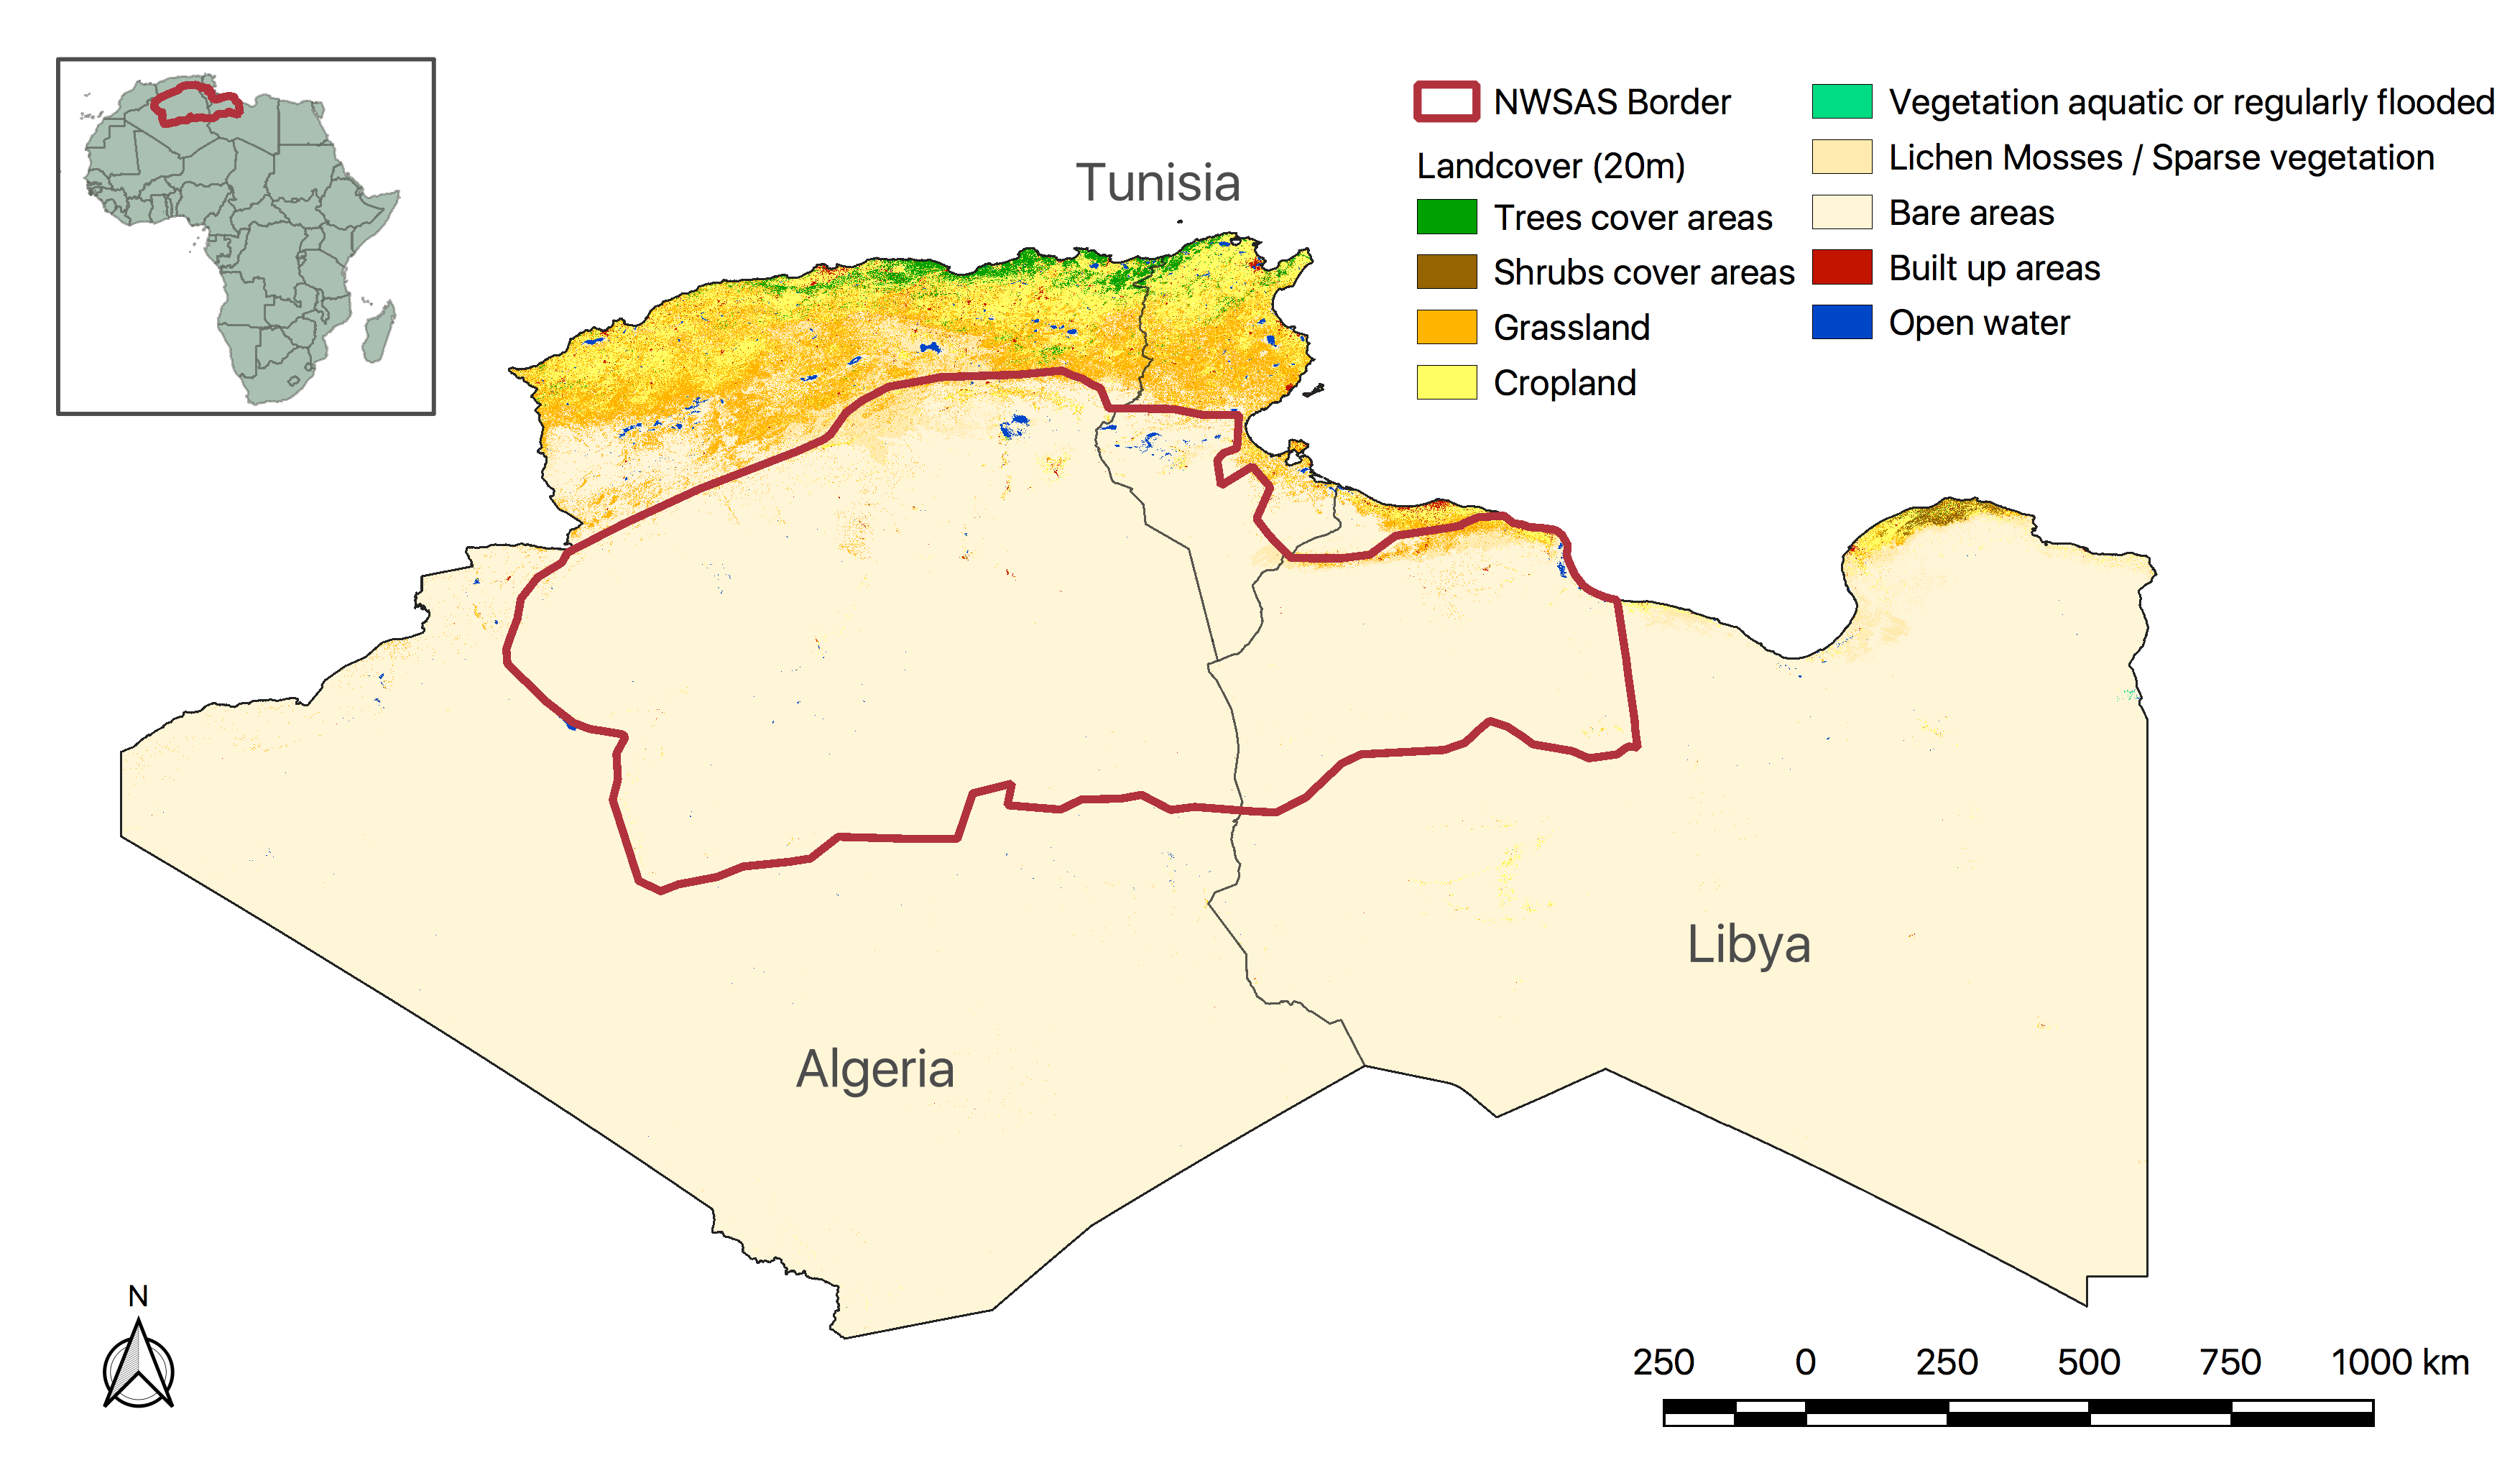
\includegraphics[width=0.9\textwidth]{NWSAS_Landcover}
	\caption[NWSAS land-cover map]{North Western Sahara Aquifer System - Land-cover map at 20$\times$20 meters grid cell resolution.}
	\label{fig:landcover}
\end{figure}

\begin{figure}[!t]
	\centering
	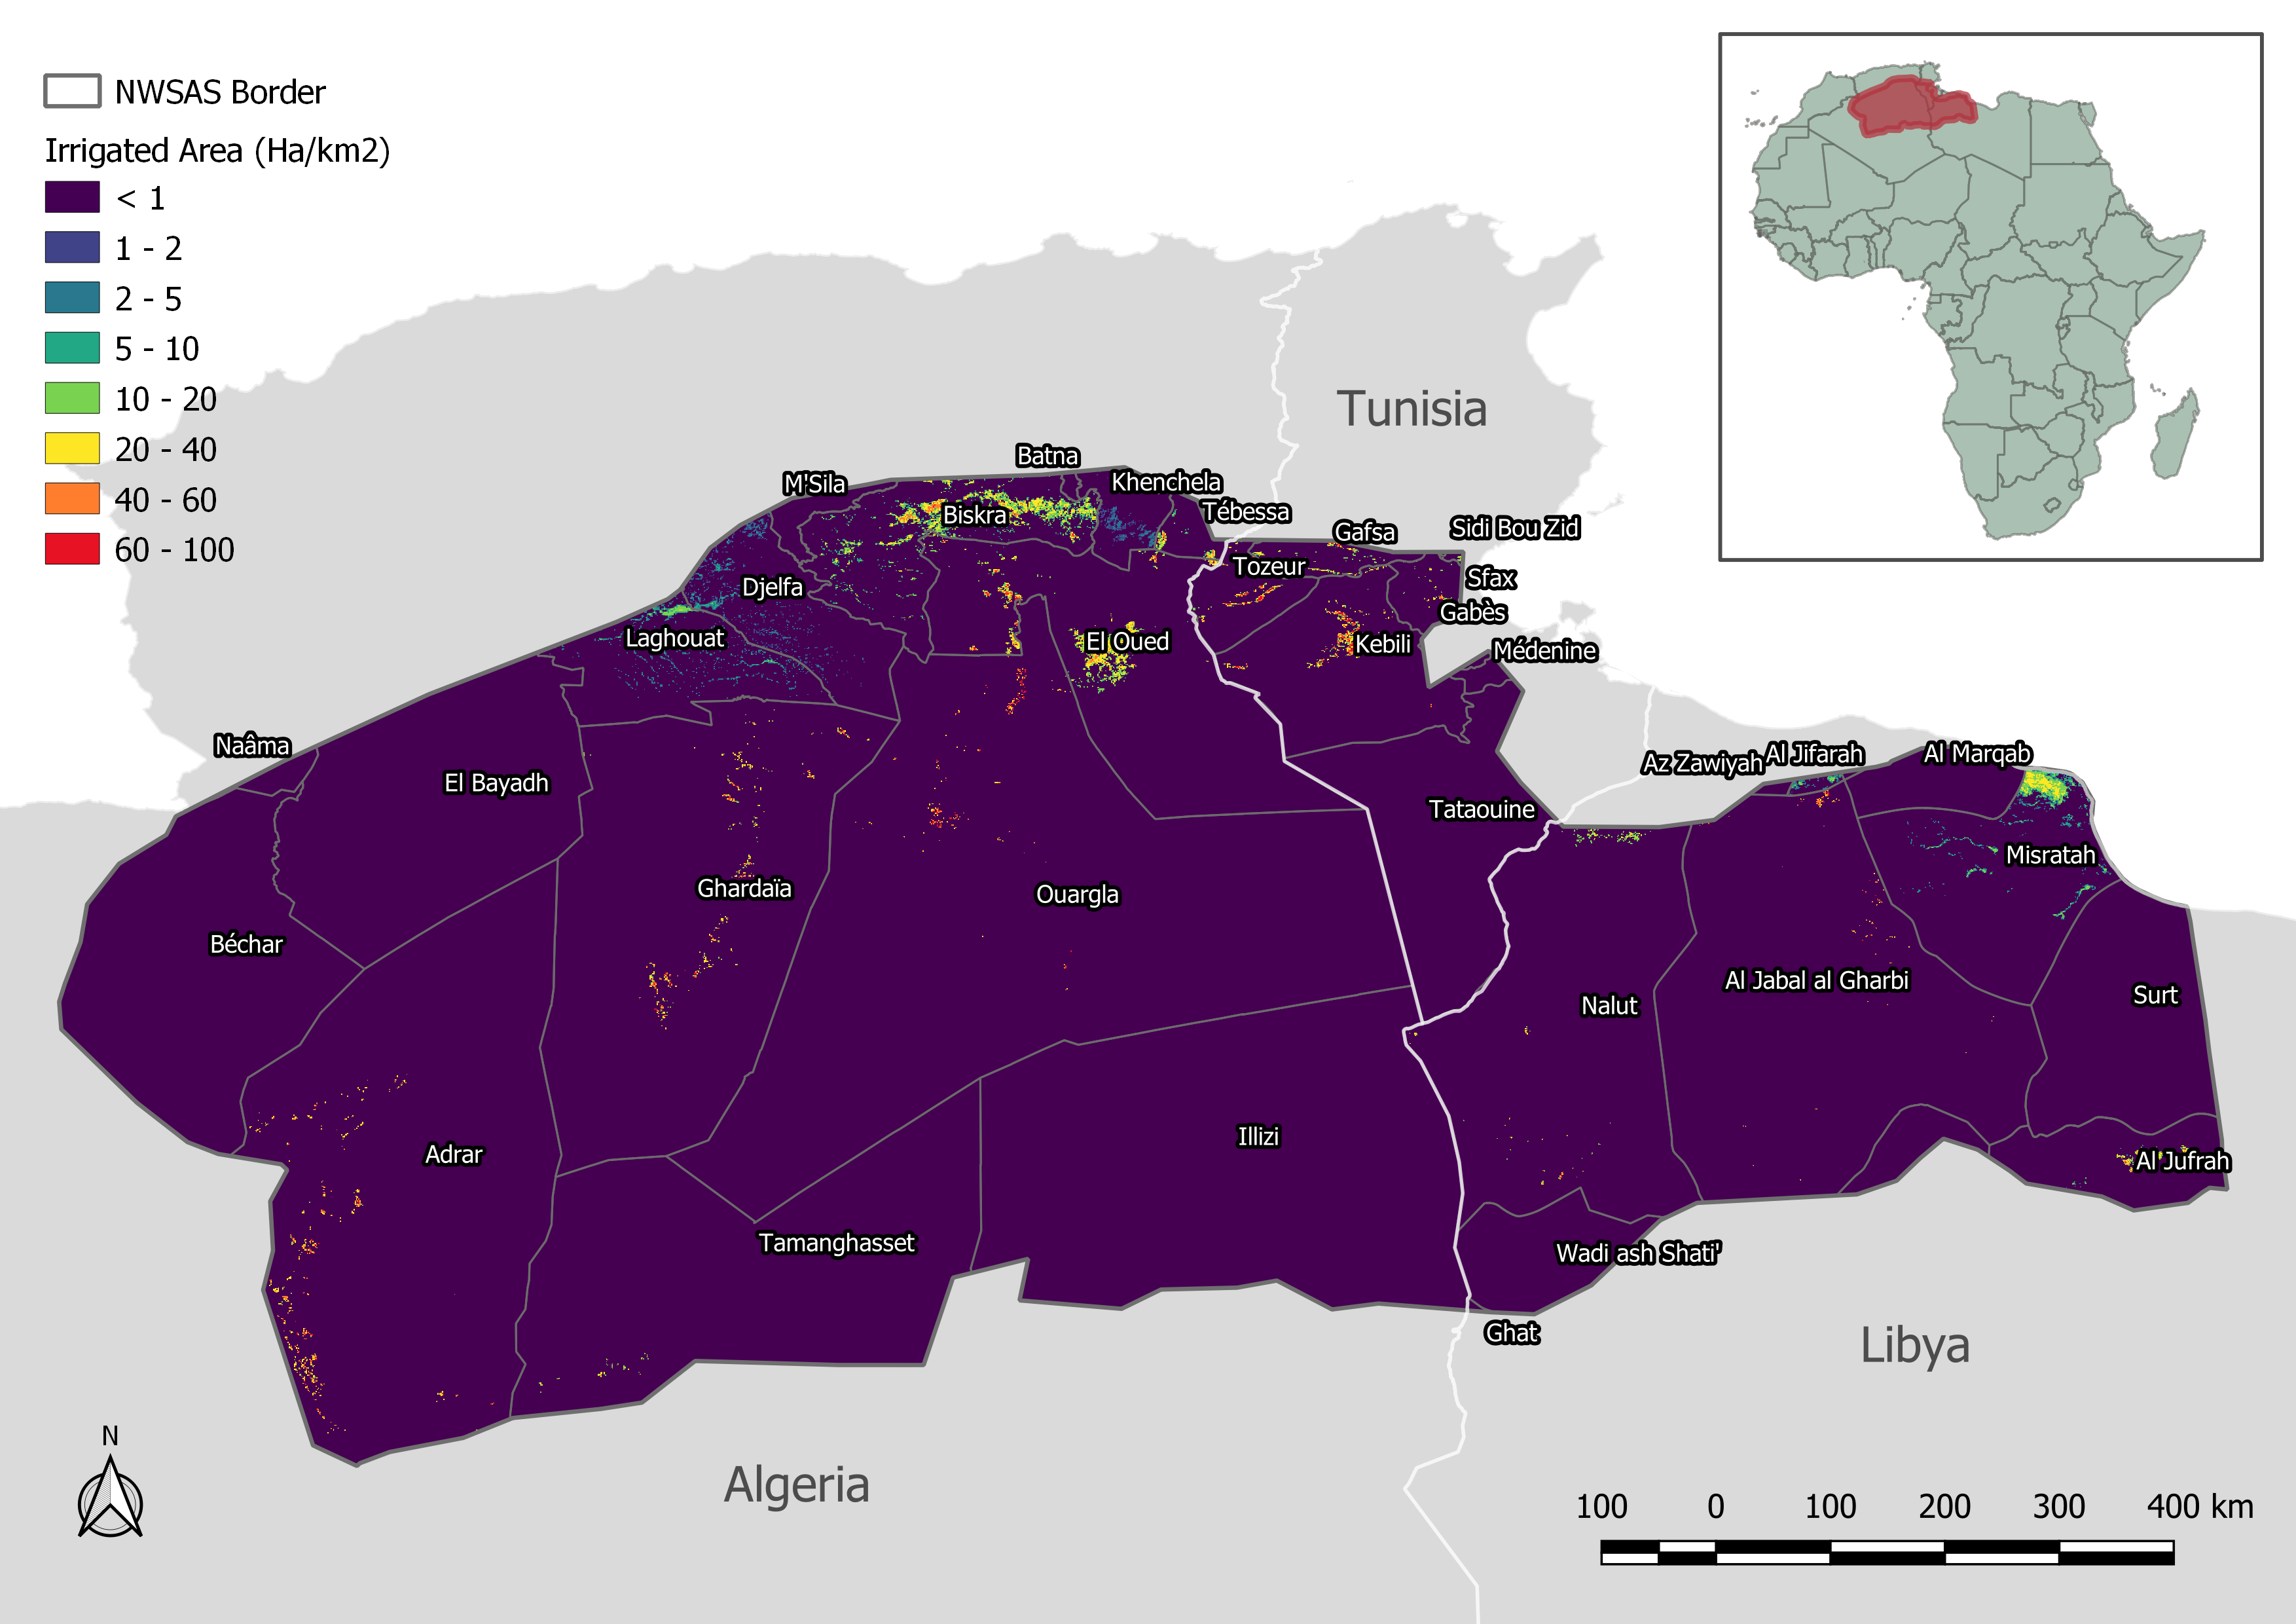
\includegraphics[width=0.88\textwidth, cfbox=black 1pt 0pt]{NWSAS_Irrigated_area}
	\caption[NWSAS cropland density map]{North Western Sahara Aquifer System - Cropland density map at 1$\times$1 km grid cell resolution.}
	\label{fig:irrigated_area}
\end{figure}

From this dataset, some insights can already be obtained. Bare/desertic areas dominate the region, while open water bodies are quite uncommon, however, the water bodies found in the NWSAS region do not constitute ``fresh water" resources due to their high content of salinity \cite{CHAOUKI20131043}. The built up areas are highly scattered throughout the NWSAS region as well as the cropland zones, which are mainly located in the surroundings of the built up areas and in the north of the region. The largest agricultural activity, is given at the north of the three countries, as well as the major urban concentrations, nonetheless, this does not make the NWSAS region less important, as the groundwater resources there, are crucial for ensuring food security for a growing population in the region.

From this land-cover dataset, the cropland areas were subtracted, allowing to create a raster layer containing the cropland density in the region. This layer was created for a resolution of 1km grid cell and calibrated for year 2015 according to regional statistics presented in \autoref{tbl:provincialdata}. The obtained cropland dataset is showcased in \autoref{fig:irrigated_area}.

From \autoref{fig:irrigated_area}, it is depicted with more clarity that the main agricultural activity is in fact, presented in the northern region. The provinces with largest agricultural activity are: Biskra, El Oued, Ouargla, Adrar and Gharda\"\i a in Algeria; Kebili and Tozeur in Tunisia; and Misratah andAl Jabal al Gharbi in Libya.

\subsection{Population dataset}
Individual population datasets for Algeria, Tunisia and Libya were obtained from the WorldPop database \cite{Worldpop} in a resolution of 100$\times$100 meters. Afterwards, the three datasets were merged together and masked within the boundaries of the aquifer. The data was then rescaled to a 1 km grid cell resolution and calibrated for year 2015 according to regional statistics (refer to \autoref{tbl:regionalstats}).

\begin{figure}[!ht]
	\centering
	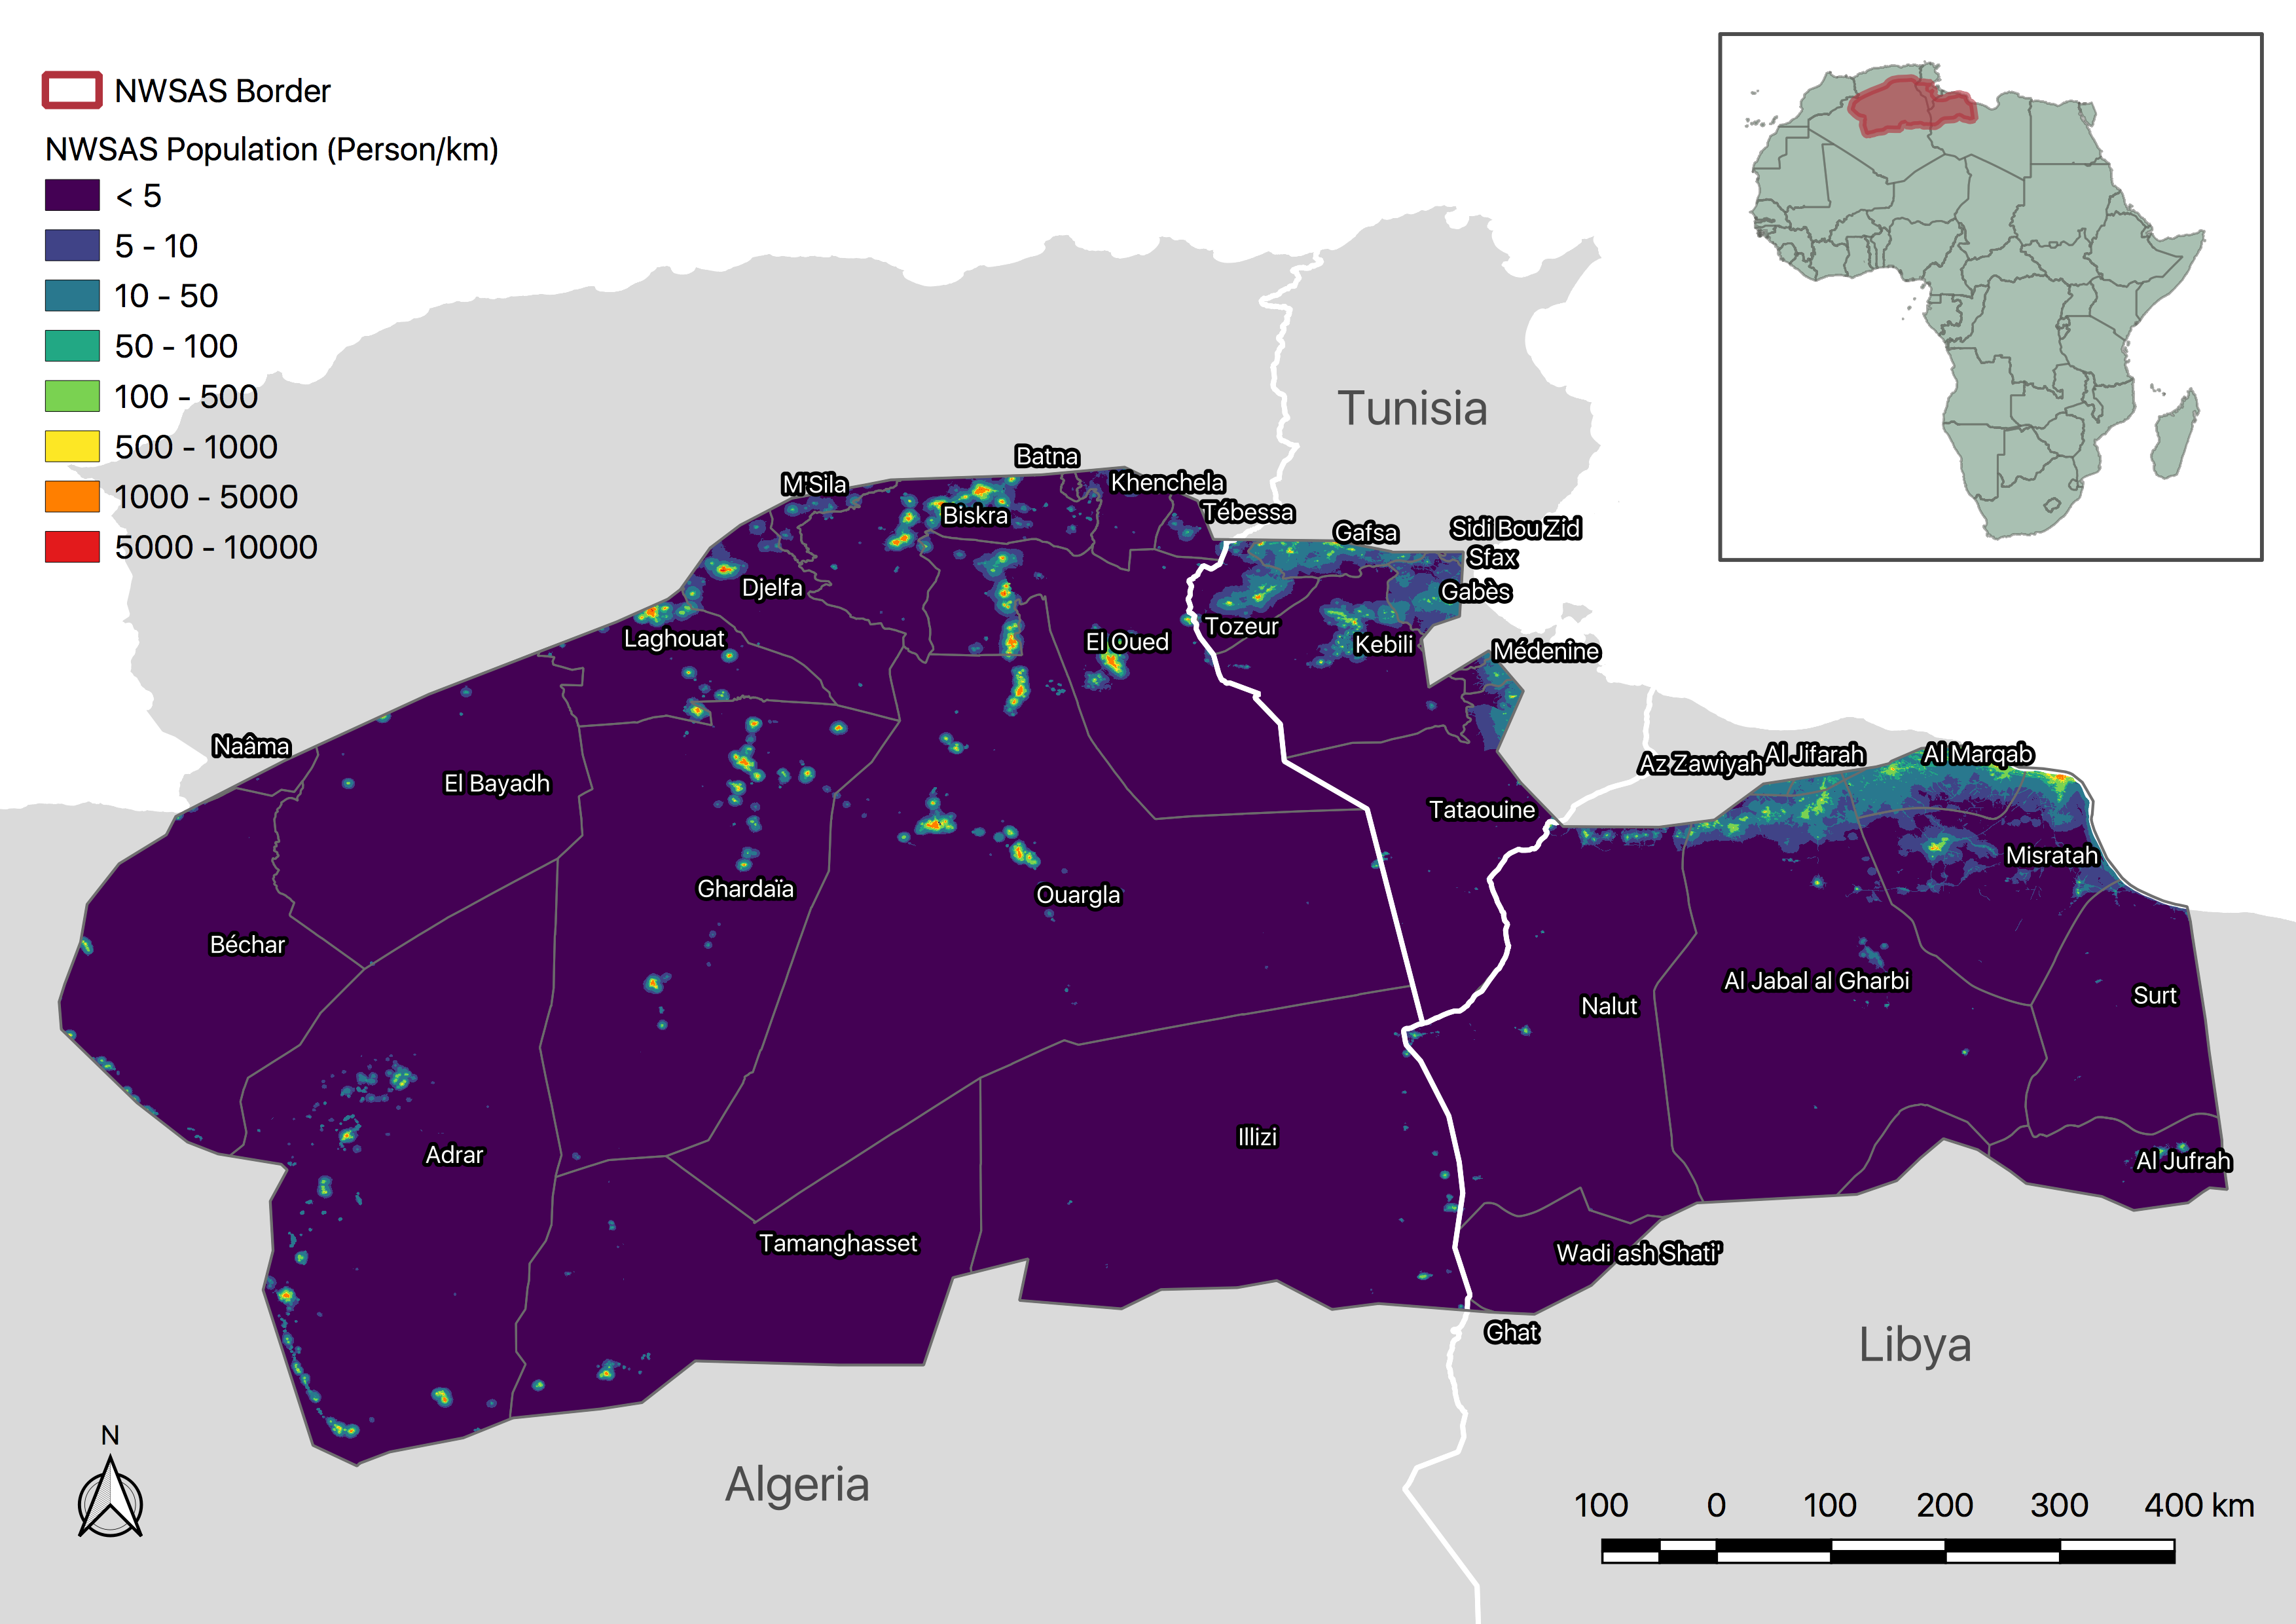
\includegraphics[width=0.88\textwidth, cfbox=black 1pt 0pt]{NWSAS_Population}
	\caption[NWSAS population map]{North Western Sahara Aquifer System - Population density map at 1$\times$1 km grid cell resolution.}
	\label{fig:population}
\end{figure}

\autoref{fig:population} depicts the obtained population layer for the NWSAS region. It is clear that the population agglomerations follow the same location pattern as the cropland areas: scattered through the region with higher concentrations at north of the aquifer. Within Algeria, the provinces with major population count are: Biskra , El Oued, Ouargla, Laghouat, Gharda\"\i a, Adrar and Djelfa. As for Tunisia, Kebili, Tozeur and Gafsa present the higher population counts, although much lower than the Algerian provinces previously mentioned. Moreover, the provinces with higher population count within Libya are Al Marqab, Misratah and Al Jabal al Gharbi.

\vfill
\subsection{Depth to groundwater dataset}
The depth to groundwater dataset used, was developed by the British Geological Survey for the African continent at a resolution of 5km grid cell. This dataset is underpinned by dedicated case studies and systematic data and literature reviews \cite{Quantitativemapsgroundwater2012a}. The dataset was masked with the NWSAS boundaries and aligned to match the target 1km grid cell resolution (\autoref{fig:depth}).

\begin{figure}[!ht]
	\centering
	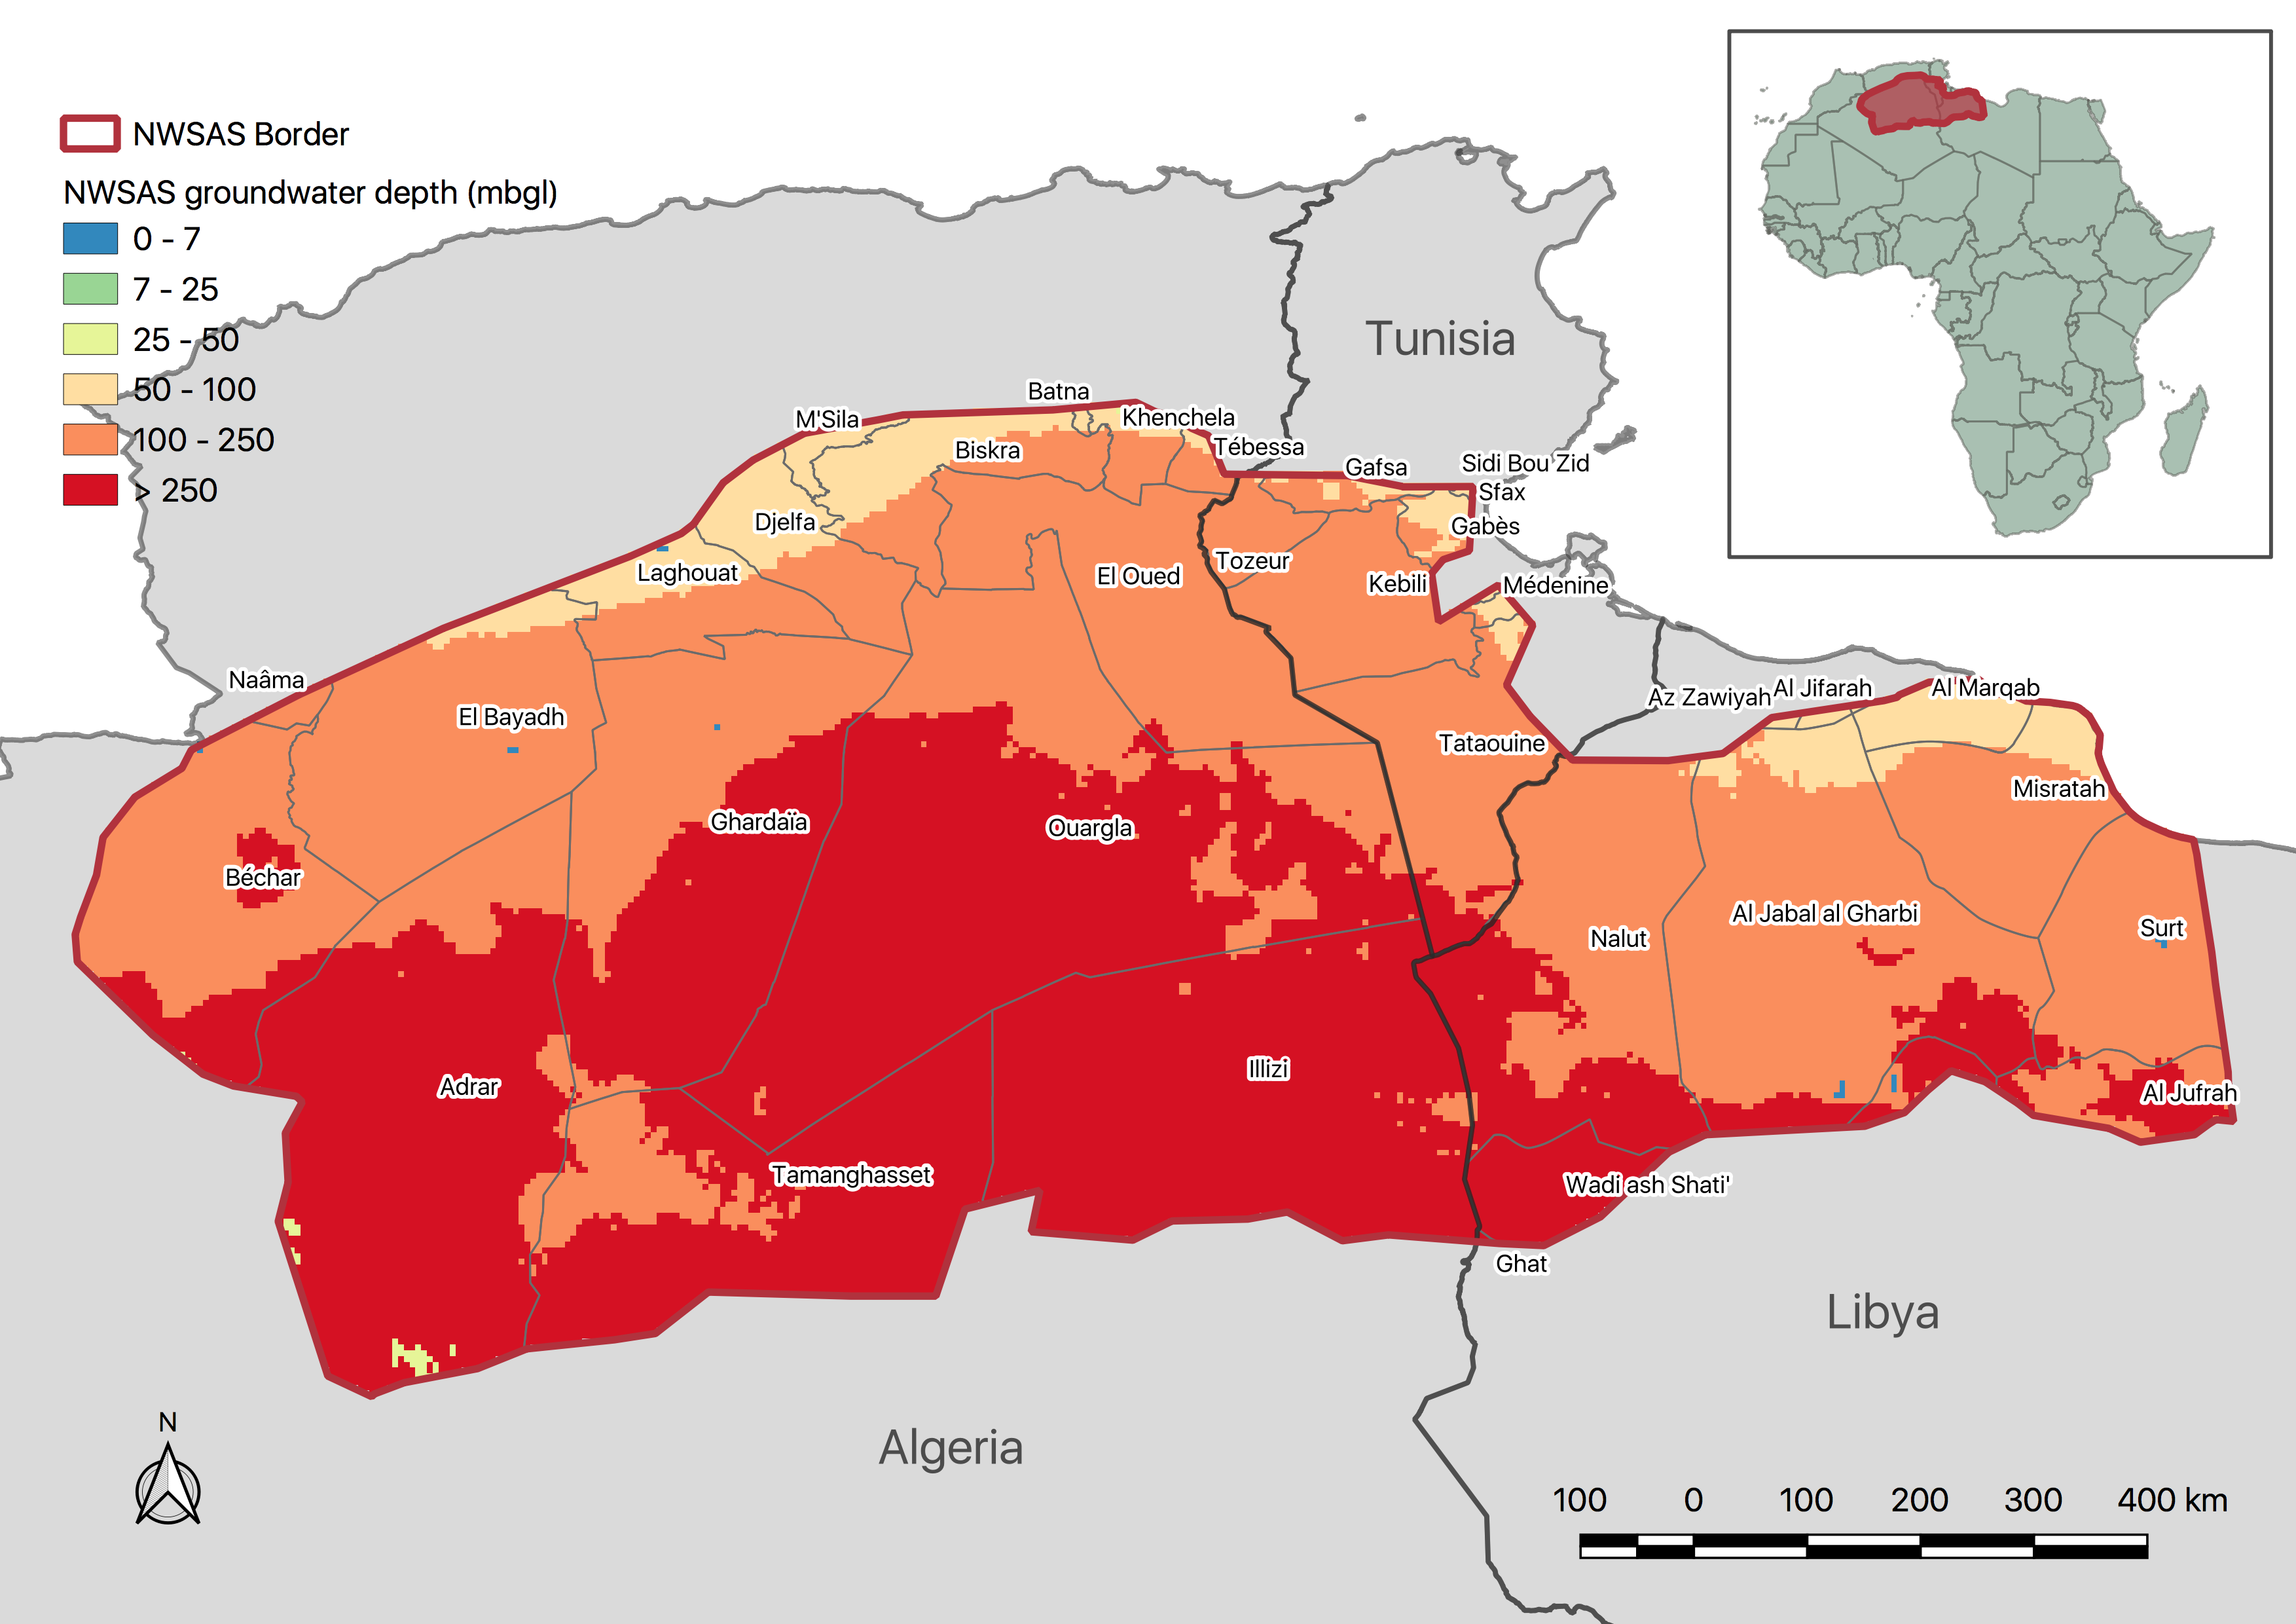
\includegraphics[width=0.88\textwidth, cfbox=black 1pt 0pt]{NWSAS_Depth}
	\caption[NWSAS depth to groundwater map]{North Western Sahara Aquifer System - Depth to groundwater map at 1$\times$1 km grid cell resolution.}
	\label{fig:depth}
\end{figure}

According to this data, it can be seen that the depth to groundwater through the entire aquifer ranges from around 50 to more than 250 meters. In general, in the south of the aquifer the deepest water tables can be found, which could mainly affect the population and agricultural activity of the province of Adrar and part of the provinces of Ouargla and Gharda\"\i a. To the north of the basin, the water table levels decrease to a range between 50 to 100 meters, which can be argued, enables the high agricultural activity there, specially in the province of Biskra.
\vfill

\section{Data calibration}
The \textit{population} and the \textit{irrigated area} layers were calibrated to match regional statistics. The calibration was performed using the fraction given between the regional statistical data (i.e. total population or total irrigated area), and the sum of all data points of the layer in question. The statistical data was available as per country or provincial basis. Thus, the calibration process was performed for the basin areas within each country/province, using their specific information (see \tref{tbl:regionalstats} and \tref{tbl:provincialdata}).

\begin{table*}[!h]
 \caption{\label{tbl:regionalstats}NWSAS population and irrigated area statistics for year 2015, subdivided per country area inside the basin. Data source: \cite{BetterValorizationIrrigation2015,Socioeconomicaspectsirrigation2014,almullaNWSAS}}
 \footnotesize
\begin{tabular}{@{}*{5}{l}}
 	\br
 	Parameter & Total & Algeria & Tunisia & Libya\\
 	\mr
 	NWSAS Population & 4,800,00 & 2,123,256 & 726,248 & 1,535,496\\
 	NWSAS Irrigated area (Ha) & 281,194 & 202,275 & 40,371 & 38,548\\
 	\br
 \end{tabular}
\end{table*}

Provincial data on irigated land was derived from \cite{abuzeidNorthWesternSahara2015,BetterValorizationIrrigation2015,Socioeconomicaspectsirrigation2014,almullaNWSAS}. Intensification rates for irrigated area were taken from \cite{Socioeconomicaspectsirrigation2014} and used to account for a growth in irrigated land to year 2050. The intensification rate measures the current average rate of irrigated area over the feasible area to be irrigated in each region. Moreover, irrigation water use per hectare values were also taken from \cite{Socioeconomicaspectsirrigation2014}, and used as basis to characterize the Baseline scenario (\tref{tbl:provincialdata}).

\begin{table*}[!h]
	\caption{\label{tbl:provincialdata}Provincial input data for irrigated area and irrigation water use. Based on \cite{abuzeidNorthWesternSahara2015,BetterValorizationIrrigation2015,Socioeconomicaspectsirrigation2014,almullaNWSAS}}
	\addtocounter{table}{-1}
\end{table*}
~\\[-50pt]
{\footnotesize
\begin{longtable}{@{}l l P{0.9in} P{0.9in} P{1in} P{0.8in}}
	\br
    Country & Province & Irrigated area (Ha) & Intensification rate (-) & Future irrigated area (Ha) & Water used (m\textsuperscript{3}/Ha)\\
	\mr
	\endfirsthead
	\multicolumn{4}{@{}l}{\ldots continued}\\\br
	Country & Province & Irrigated area (Ha) & Intensification rate (-) & Future irrigated area (Ha) & Water used (m\textsuperscript{3}/Ha)\\\mr
	\endhead % all the lines above this will be repeated on every page
	\br
	\multicolumn{4}{r@{}}{continued \ldots}\\
	\endfoot
	\endlastfoot
	Algeria & Adrar              & 28,228 & 0.84 & 33,605 & 14,518 \\
			& Batna              & -      & 0.84 & -      & 13,520 \\
			& Biskra             & 60,000 & 0.80 & 75,000 & 12,383 \\
			& Béchar             & -      & 0.84 & -      & 13,520 \\
			& Djelfa             & 3,000  & 0.84 & 3,571  & 13,520 \\
			& El Bayadh          & -      & 0.84 & -      & 13,520 \\
			& El Oued            & 50,000 & 0.80 & 62,500 & 13,023 \\
			& Gharda\"\i a           & 20,441 & 0.84 & 24,335 & 13,520 \\
			& Illizi             & -      & 0.84 & -      & 13,520 \\
			& Khenchela          & 1,000  & 0.84 & 1,190  & 13,520 \\
			& Laghouat           & 5,000  & 0.84 & 5,952  & 13,520 \\
			& M'Sila             & -      & 0.84 & -      & 13,520 \\
			& Naâma              & -      & 0.84 & -      & 13,520 \\
			& Ouargla            & 29,488 & 0.88 & 33,509 & 14,218 \\
			& Tamanghasset       & 1,118  & 0.84 & 1,331  & 13,520 \\
			& T\'ebessa            & 4,000  & 0.84 & 4,762  & 13,520 \\\ms
	Libya   & Al Jabal al Gharbi & 7,635  & 0.80 & 9,544  & 9,134  \\
			& Al Jifarah         & 1,000  & 0.80 & 1,250  & 10,193 \\
			& Al Jufrah          & 6,925  & 0.80 & 8,656  & 9,134  \\
			& Al Marqab          & -      & 0.98 & -      & 10,001 \\
			& Az Zawiyah         & -      & 0.80 & -      & 10,193 \\
			& Misratah           & 18,333 & 0.80 & 22,916 & 9,134  \\
			& Nalut              & 4,655  & 0.80 & 5,819  & 9,134  \\
			& Surt               & -      & 0.80 & -      & 9,134  \\
			& Tripoli            & -      & 0.80 & -      & 10,193 \\
			& Wadi ash Shati'    & -      & 0.80 & -      & 9,134  \\\ms
	Tunisia & Gabès              & 2,380  & 0.89 & 2,674  & 7,038  \\
			& Gafsa              & 5,441  & 0.90 & 6,046  & 13,266 \\
			& Kebili             & 23,837 & 0.98 & 24,323 & 16,813 \\
			& Médenine           & -      & 0.77 & -      & 3,633  \\
			& Sfax               & 350    & 0.90 & 389    & 13,266 \\
			& Tataouine          & -      & 0.77 & -      & 3,633  \\
			& Tozeur             & 8,363  & 0.98 & 8,534  & 16,813 \\
	\br
\end{longtable}
}

\vfill
\section{Domestic and irrigation water withdrawals}
The calculation of total water withdrawals $ww_{tot,i}$ was performed according to \Eref{eq:waterwithdrawals}. Domestic water withdrawals were calculated as the product between the population count in each data cell ($Pop_{i}$) and the specific water demand per capita ($wpc_{i}$) for the region. Similarly, withdrawals from irrigated agriculture were calculated as the product between the irrigated area inside each data cell ($IrrArea_{i}$) and the specific water demand per cultivated hectare ($wpha_{i}$) for the region.

\begin{equation}\label{eq:waterwithdrawals} 
 ww_{tot,i} = Pop_{i}\cdot wpc_{i} +IrrArea_{i}\cdot wpha_{i} 
\end{equation}

For the Baseline, a level of water withdrawals per capita $wpc$ of 55 cubic meters per year was assumed with a population growth of 0.5\% per year \cite{Householdwaterconsumption2014}. Moreover, all cropland area resultant from the calibration process was considered to be irrigated by groundwater resources in accordance with data from \cite{abuzeidNorthWesternSahara2015} (see \tref{tbl:watersources}) and the water requirements per cultivated hectare $wpha$ to be according to \tref{tbl:provincialdata}. Moreover, these values are changed depending on the irrigation water regime of each scenario. Finally, a growth in irrigated area was considered based on the intensification rate reported for each province (\tref{tbl:provincialdata}).

\begin{table*}[!h]
	\caption{\label{tbl:watersources}Irrigated and rain-fed cropland area in the NWSAS, year 2012. Data source: \cite{abuzeidNorthWesternSahara2015}}
	\footnotesize
	\begin{tabular}{@{}*{5}{l}}
		\br
		Water and land use & Whole aquifer & Algeria & Tunisia & Libya\\
		\mr
		Irrigated agricultural land (Ha) & 270,000 & 202,000 & 30,000 & 38,000\\
		Rain-fed agricultural land (Ha) &  &  & 102,000 & 133,300\\
		\br
	\end{tabular}
\end{table*}

\section{Groundwater pumping}\label{Sc:pumping}
The energy needs to pump water from groundwater resources is given by the required lift ($H-h$), the pressure drop due to fluid friction in the piping, and the pressure losses in valves and fittings. Pressure losses due to friction in the piping were found to be rather small compared to the lift requirements. Therefore, and due to lack of specific data on wells and boreholes in the region, the pressure losses due to friction in the piping and in valves and fittings were disregarded. The energy requirements (in watt-h) can then be estimated as \eref{eq:1} \cite{Groundwaterdependentirrigationcosts2017}:

\begin{equation}\label{eq:1}
E = \frac{Q\cdot(\rho\cdot g\cdot(H - h))}{\eta}
\end{equation}

Where $Q$ stands for the water extractions (m\textsuperscript{3}), $\rho$ for the water density (kg/m\textsuperscript{3}), $g$ for the gravitational acceleration (m/s\textsuperscript{2}), $H$ for the delivered hydraulic head (meters), and $h$ for the head in the well (meters). Moreover, $\eta$ accounts for the pumping efficiency, which was set as 85\% along the entire aquifer.

\section{Energy-for-wastewater}\label{Sc:eww}
To calculate the energy-for-wastewater requirements an energy intensity factor was used for each evaluated treatment technology following \eref{eq:energy-for-wastewater}.

\begin{equation}\label{eq:energy-for-wastewater}
E_{ww} = Q_{ww,yr}\cdot X_t
\end{equation}

Where $Q_{ww,yr}$ represents the yearly treated wastewater in m\textsuperscript{3}/yr, and $X_t$ the average energy demand of the specific WWTT $t$, to treat one m\textsuperscript{3} of wastewater (in kWh/m\textsuperscript{3}).

\section{Wastewater Treatment System characteristics}
FAO standards for population wastewater pollutant levels and reused water quality for agricultural irrigation \cite{fao1985water}, were used for the entire NWSAS area. These are shown in \tref{tbl:pollutans}.

\begin{table*}[!ht]
	\caption{\label{tbl:pollutans}Pollutant levels of domestic wastewater and treated wastewater to be reused in agricultural irrigation. Based on \cite{fao1985water}.}
	\footnotesize
		\begin{tabular}{@{}*{4}l}
			\br
			Pollutant type & Domestic (mg/l) & Treated (mg/l) & Removal (\%)\\
			\mr
			Suspended solids ($SS$) & 700 & 30 & 95\%\\
			Nitrogen ($N$) & 40 & 30 & 25\%\\
			Phosphorus ($P$) & 20 & 10 & 50\%\\
			Biochemical Oxygen Demand ($BOD_5$) & 500 & 50 & 90\%\\
			Chemical Oxygen Demand ($COD$)& 1300 & 120 & 90\%\\
			\br
		\end{tabular}
\end{table*}

Cost functions for different WWTT taken from the work of \citet{Assessmentwastewatertreatment2012}, were used to evaluate the competence of selected technologies in the NWSAS. Energy intensity characteristics were added for each technology according to \cite{Energypatternanalysis2012,ComparativeAnalysisEnergy2017}. The characteristics of the different WWTT and their cost and energy functions are presented in \tref{tbl:treatmentsystems}.

\begin{table*}[!h]
    \caption{\label{tbl:treatmentsystems}Treatment systems analyzed Adapted from \cite{Assessmentwastewatertreatment2012}, Copyright (2012), with permission from Elsevier.}
    \addtocounter{table}{-1}
\end{table*}
	~\\[-50pt]{\footnotesize
	\begin{longtable}{@{}P{1.2in} P{0.9in} P{1.9in} P{0.7in} P{0.7in}}
	\br
    Technology & Pollutant removal (\%) & Costs (\euro) & Energy (kWh)$^{\dagger}$ & Usage\\
    \mr
    \endfirsthead
    \multicolumn{4}{@{}l}{\ldots continued}\\\br
    Technology & Pollutant removal (\%) & Costs (\euro) & Energy (kWh)$^{\dagger}$ & Usage\\\mr
    \endhead % all the lines above this will be repeated on every page
    \br
    \multicolumn{4}{r@{}}{continued \ldots}\\
    \endfoot
    \endlastfoot
    Pond System (PS) & N: 20 -- 40 \newline P: 60 -- 70 \newline COD: 60 -- 96 \newline SS: 50 -- 90 & CAPEX: $3897.7\cdot x^{-0.407}$ \newline OPEX: $5.543\cdot x + 3127.5$ & $0.19\cdot V$ & Irrigation tailwater\\
    Intermittent Sand Filter (ISF) & N: 65 -- 95 \newline P: 75 -- 99 \newline COD: 75 -- 90 \newline SS: 85 -- 95 & CAPEX: $2115.5\cdot x^{-0.399}$ \newline OPEX: $12.026\cdot x+3518.9$ & $0.2\cdot V$ & Domestic wastewater\\
    Trickling Filter (TF) & N: 35 -- 50 \newline P: 35 -- 55 \newline COD: 75 -- 90 \newline SS: 50 -- 90 & CAPEX: $12237\cdot x^{-0.87}$ \newline OPEX: $13.504\cdot x+6020$ & $0.3\cdot V$ & Domestic wastewater\\
    Moving Bed Biofilm Reactor (MBBR) & N: 10 -- 20 \newline P: 30 -- 40 \newline COD: 20 -- 40 \newline SS: 60 -- 80 & CAPEX: $1187\cdot x^{-0.165}$ \newline OPEX: $12.794\cdot x+6031$ & $0.8\cdot V$ & Domestic wastewater\\
    Rotating Biological Contractors (RBC) & N: 20 -- 80 \newline P: 10 -- 30 \newline COD: 70 -- 93 \newline SS: 75 -- 98 & CAPEX: $6931.4\cdot x^{-0.383}$ \newline OPEX: $313.4\cdot x^{-0.435}$ & $0.8\cdot V$ & Domestic wastewater\\
    Membrane Bioreactor (MBR) & N: 50 -- 90 \newline P: 20 -- 70 \newline COD: 70 -- 90 \newline SS: 85 -- 99 & CAPEX: $5635.3\cdot x^{-0.352}$\newline $^{*}$OPEX: $2.116\cdot V^{0.713}e^{1.51\cdot SS+0.037\cdot BOD}$ & $0.8\cdot V$ & Domestic wastewater\\
    Extended Aeration (EA) & N: 50 -- 90 \newline P: 15 -- 70 \newline COD: 70 -- 90 \newline SS: 85 -- 99 & CAPEX: $7946\cdot x^{-0.460}$ \newline $^{*}$OPEX: $169.48\cdot V^{0.454}e^{0.61\cdot SS}$ & $0.6\cdot V$ & Domestic wastewater\\
    Sequencing Batch Reactor (SBR) & N: 55 -- 90 \newline P: 25 -- 70 \newline COD: 70 -- 90 \newline SS: 85 -- 99 & CAPEX: $8258.9\cdot x^{-0.407}$ \newline OPEX: $309.4\cdot x^{-0.389}$ & $1\cdot V$ & Domestic wastewater\\
    \br
    \multicolumn{4}{@{}l}{$x$: population equivalent, $x=V\times1500/(400\times365)$, $V$: wastewater flow (m\textsuperscript{3}/yr)} \\
    \multicolumn{4}{@{}l}{N: Nitrogen, P: Phosphorus, COD: Chemical Oxygen Demand, SS: Suspended Solids} \\
    \multicolumn{4}{@{}l}{CAPEX: Capital Expenditure, OPEX: Operating Expenses}\\
    $^{*}$ Taken from \cite{Costmodellingwastewater2011} & & & \\ 
    $^{\dagger}$ Based on \cite{Energyrequirementswater2012,ComparativeAnalysisEnergy2017} & & & 
    \end{longtable}
	}

\section{Reverse Osmosis desalination}\label{Sc:RO}
Reverse Osmosis (RO) desalination is the most popular desalination technology used worldwide. Its energy intensity falls typically in the range of 0.5 to 2.5 kWh per cubic meter of desalinated brackish water \cite{Energyoptimalgroundwater2013,karabelasAnalysisSpecificEnergy2018a,panBrackishWaterDesalination2020}.

To estimate the energy required to desalinate one cubic meter of saline water, often detailed information of the RO system is required. When analysing a broad area using a geospatial approach, such information is not available as the characteristics of the system can change from application to application \cite{stillwellPredictingSpecificEnergy2016,aminfardMultilayeredSpatialMethodology2019}. Thus, a simplified approach was used to estimate the RO energy requirements. RO is a pressure-driven process that forces water through a membrane which separates dissolved solutes using preferential diffusion. The output water from the membrane (\textit{permeate, p}) is relatively free of solutes, while the remaining water (\textit{concentrate, c}) exits the pressure vessel with a high concentration of solutes (i.e. high TDS levels). A schematic representation of the process is presented in \fref{fig:ro} \cite{crittenden_mwhs_2012}.

\begin{figure}[!h]
	\centering
	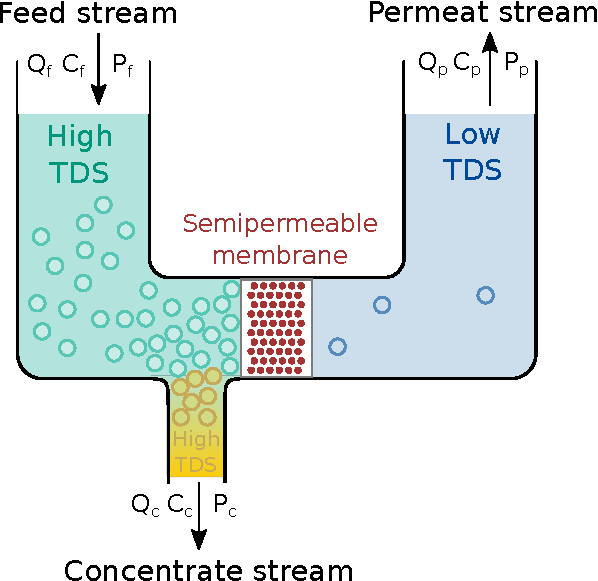
\includegraphics[width=0.4\textwidth]{Reverse_Osmosis}
	\caption[Reverse Osmosis schematic separation process]{Reverse osmosis schematic separation process. Based on: \cite{crittenden_mwhs_2012}.}
	\label{fig:ro}
\end{figure} 

The minimum energy required to push the water through the membrane is given by the amount of diluted solutes in the \textit{feed (f)} water. Such minimum energy can be estimated calculating the osmotic pressure of the \textit{feed} water, as described in \eref{eq:6} \cite{crittenden_mwhs_2012}.

\begin{equation}\label{eq:6}
\pi = \phi\cdot C\cdot R\cdot T
\end{equation}

\noindent{Where}:
\begin{itemize}[label={-}]
	\item $\pi$: osmotic pressure (bar),
	\item $\phi$: osmotic coefficient, close to 1 (-), assumed a 0.95 \cite{crittenden_mwhs_2012},
	\item $C$: concentration of all solutes (mol/L),
	\item $R$: universal gas constant, 0.083145 (L$\cdot$bar/mol$\cdot$K),
	\item $T$: absolute temperature (K), (273 + \degree C), assumed at 25 \degree C for the entire aquifer.
\end{itemize}~

Thus, the minimum energy demand can be estimated multiplying the osmotic pressure of the \textit{feed} water $\pi$ (in bar) by a conversion factor of 1.0 kWh/m\textsuperscript{3} = 36 bar and the \textit{feed} brakish volum per year $Q_y$. 

\begin{equation}\label{eq:7}
SEC_{min} = 36 \cdot \pi \cdot Q_y
\end{equation}

In reality, the energy demanded is greater due to factors as friction losses, membrane filtration resistance, among others \cite{karabelasAnalysisSpecificEnergy2018a,panBrackishWaterDesalination2020}. Thus, values were taken from \cite{karabelasAnalysisSpecificEnergy2018a} to account for the additional energy needs.

\begin{table*}[!ht]
	\caption{\label{tbl:rodesal}Energy requirements for brackish water RO desalination. Adapted from \cite{karabelasAnalysisSpecificEnergy2018a}, Copyright (2018), with permission from Elsevier.}
	\footnotesize
	\begin{tabular}{@{}*{2}l}
		\br
		Itemized SEC (kWh/m\textsuperscript{3}) & Brackish water\\
		\mr
		$SEC_f$ membrane filtration resistance & 0.194\\
		$SEC_R$ friction losses, retentate & 0.036\\
		$SEC_P$ friction losses, permeate & 0.0016\\
		$SEC_CP$ concentration polarizatione & 0.005\\
		$SEC_inef$ pump \& ERD inefficiency & 0.068\\
		\br
	\end{tabular}\\
	ERD: energy recovery device
\end{table*}

\begin{figure*}[!h]
	\centering
	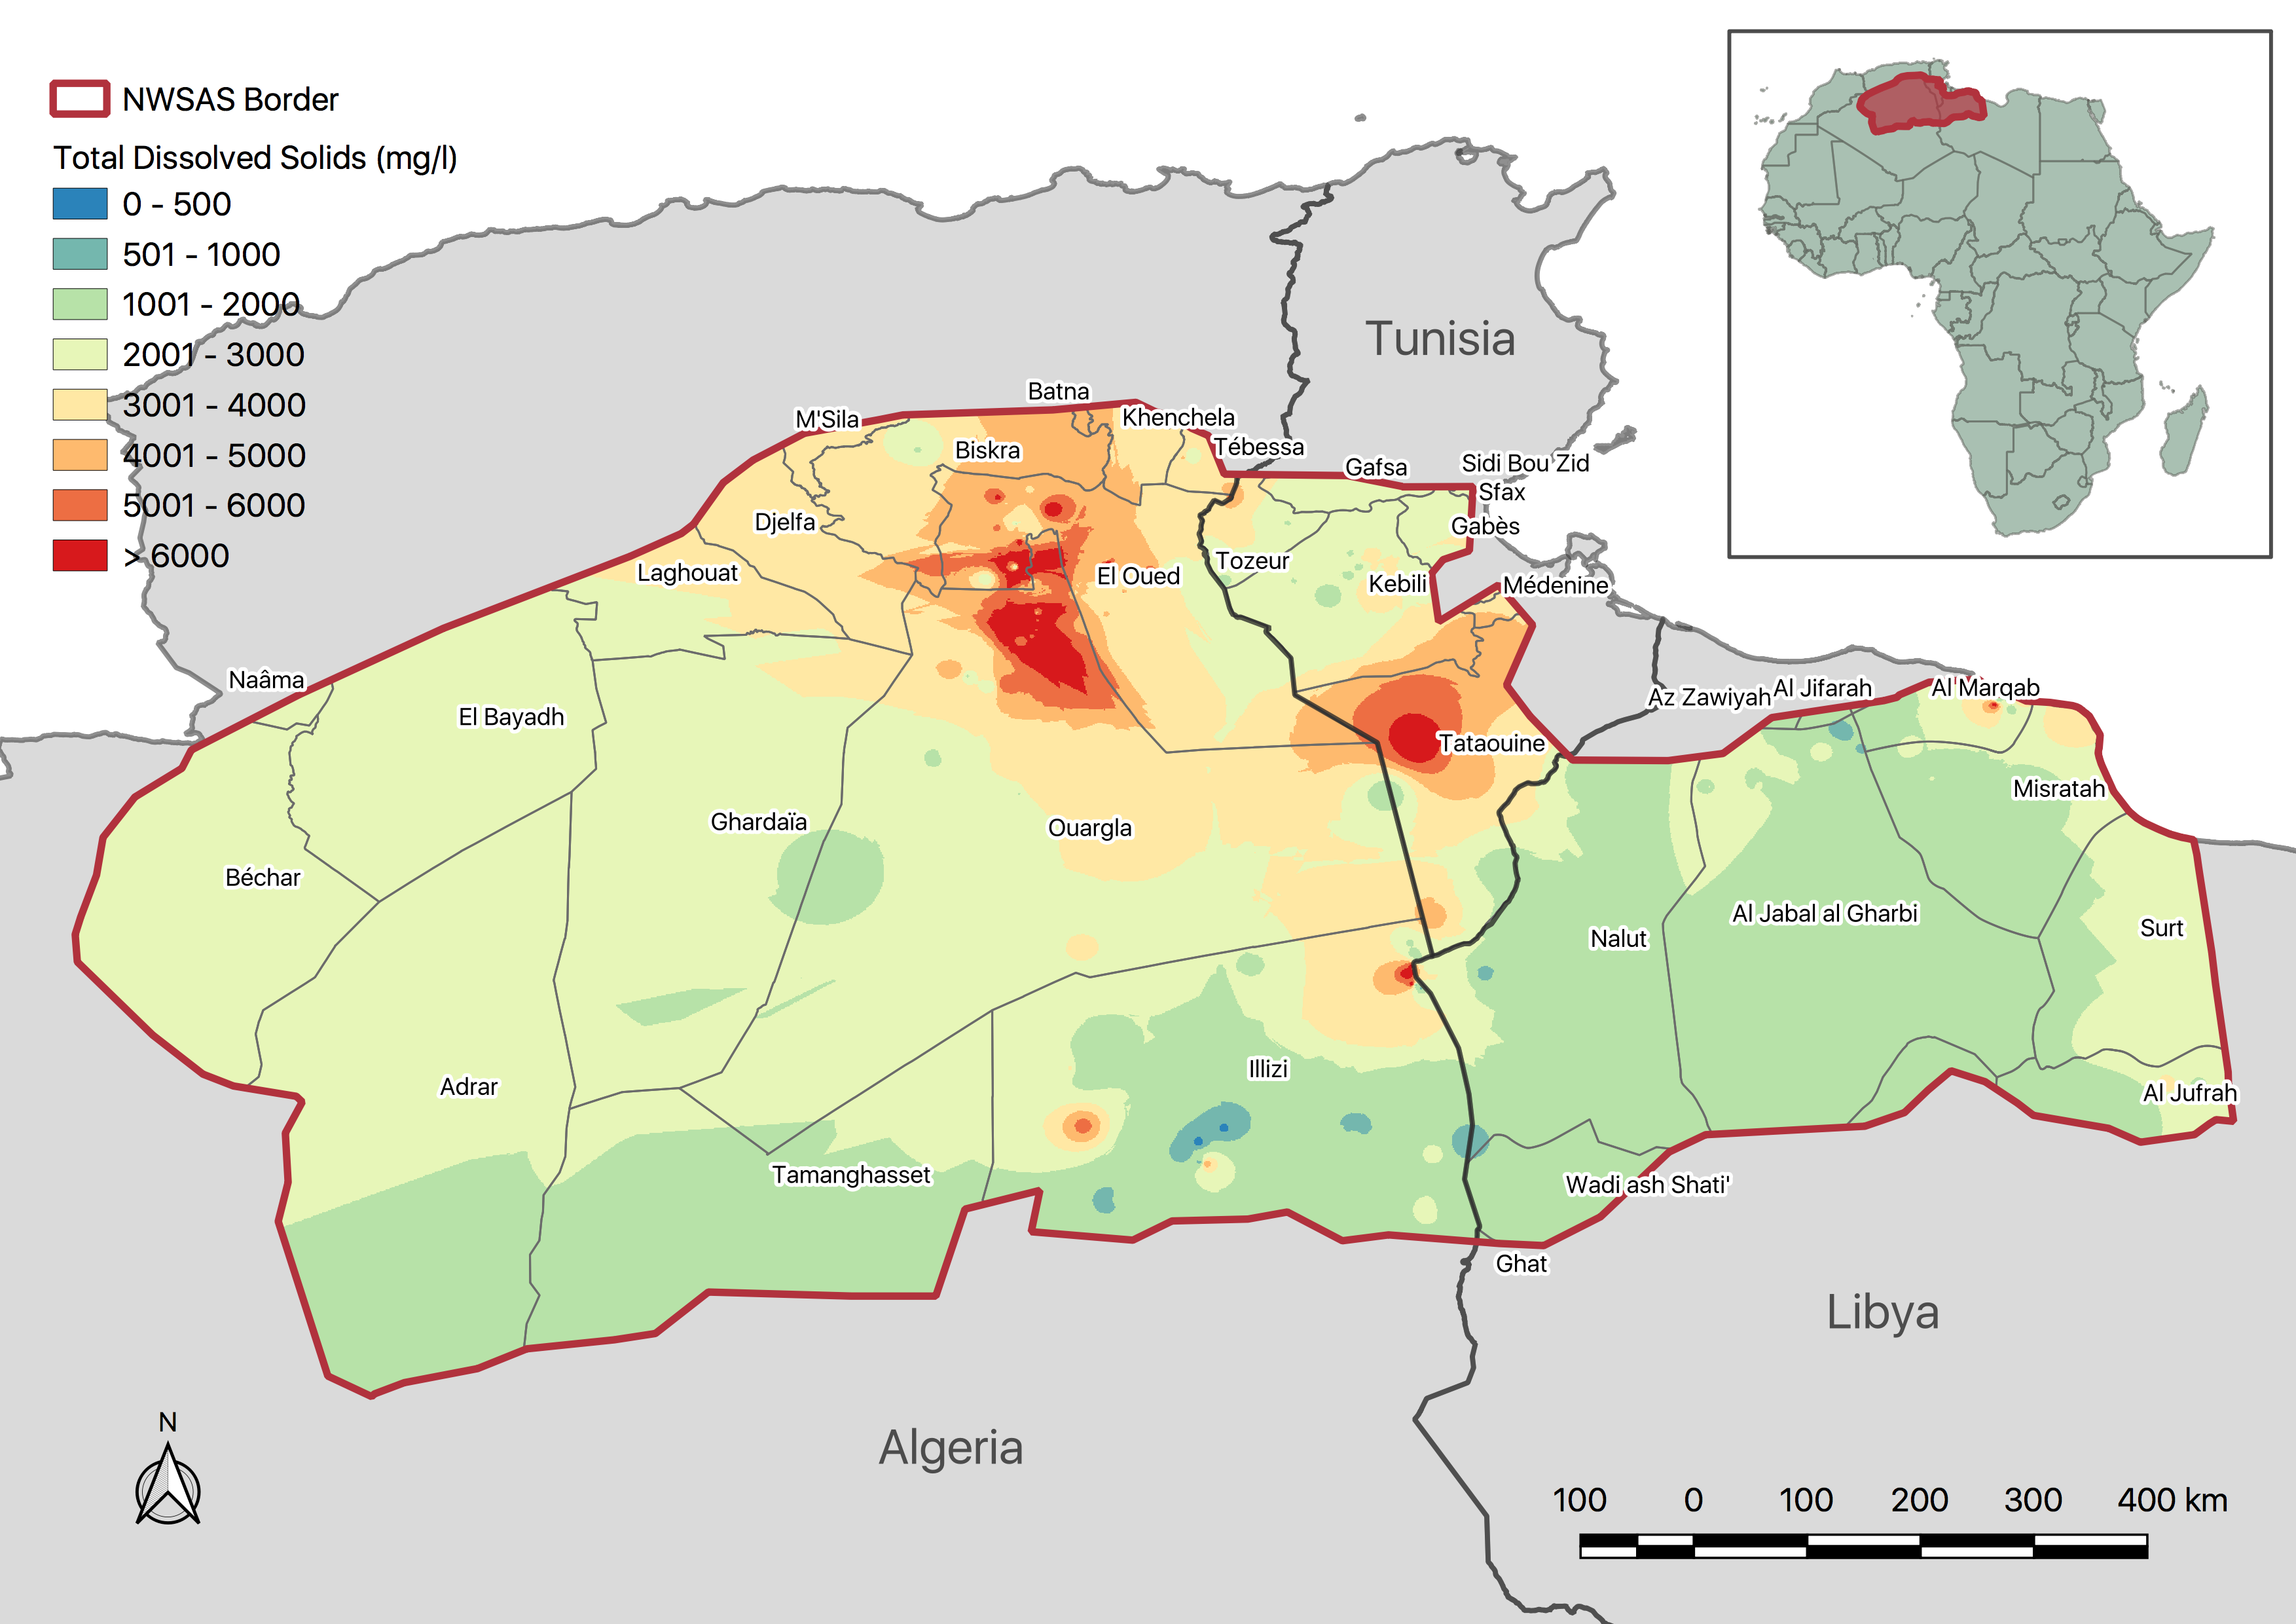
\includegraphics[width=0.88\textwidth, cfbox=black 1pt 0pt]{NWSAS_TDS}
	\caption[NWSAS groundwater quality map - Total Dissolved Solids (TDS)]{North Western Sahara Aquifer System - Groundwater quality map, Total Dissolved Solids (TDS) at 1$\times$1 km grid cell resolution.}
	\label{fig:TDS}
\end{figure*}

Moreover, brine post treatment is key to prevent environmental impacts, such as water and soil salinization \cite{panBrackishWaterDesalination2020}. However, brine treatment and disposal can be an expensive process, therefore proper processes need to be design accounting for the region characteristics \cite{panBrackishWaterDesalination2020}. 

The water quality layer used, was obtained from 206 measurements provided by National Authorities of the region. Each point specifies the spacial location and groundwater TDS content. Although the data did not covered the entire basin area, due to lack of any other related information it was used to produced a raster layer. An inverse distance weighted interpolation method, having as distance weighting factor an inverse distance to a power of 2 and a global search radius with maximum number of nearest points of 10 was used (see \fref{fig:TDS}).

\section{Levelised Cost of Water (LCOW)}
In this section the LCOW methodology is expanded as it could be beneficial for future work on the subject. This could aid on understanding what would be the efforts required as tax deductions, subsidies or reduced interest loans, for treated wastewater/tailwater to be competitive with local costs of water (what the farmer actually pays). The goal in the manuscript was to provide an overall picture, thus efforts could be concentrated in regions with high potential.

\autoref{eq:lcow}, disaggregates the $LCOW$ (\$/m\textsuperscript{3}) value in three components: the cost components due to investment $LCOW_{Inv}$, operation and maintenance $LCOW_{O\&M}$ and externalities $LCOW_{Ext}$.

\begin{equation}\label{eq:lcow}
LCOW = LCOW_{Inv} + LCOW_{O\&M} + LCOW_{Ext}
\end{equation}

All investment components used, need to be comprised in the CAPEX function of each WWTT. This enables the use of the values calculated with the CAPEX functions of each WWTT for each region or cluster, to easily calculate the $LCOW_{Inv}$ values for each specific technology and region/cluster. \autoref{eq:lcow_inv} describes the process to calculate the $LCOW_{Inv}$.

\begin{equation}\label{eq:lcow_inv}
LCOW_{Inv} = \frac{Inv}{\sum_{t=1}^{T} V_{t}\cdot\gamma^{t}}\cdot\Delta
\end{equation}

Where $Inv$ stands for the CAPEX value, $V_{t}$ for the treated water flow per year $t$ (m\textsuperscript{3}/yr), $\Delta$ for the tax factor (\autoref{eq:delta}) and $\gamma^{t}$ represents the discount factor of the project (\autoref{eq:gamma}).

The discount factor is an important term, as the LCOW methodology represents a break-even investment for the stakeholders, thus an appropriate discount rate ($r$) needs to be used to ensure the right amount of return needed for all sources of long term capital (i.e. equity holders and debt). Often, the proper discount rate used is the WACC \cite{prospectscostcompetitive2013}. The discount factor is then calculated according to the discount rate $r$, as shown in \eref{eq:gamma}. A discount rate of $r=5\%$ was used for this study, with a sensitivity analysis on lower (3\%) and higher (8\%) values.

\begin{equation}\label{eq:gamma}
\gamma^{t} = \left(\frac{1}{1+r}\right)^{t}
\end{equation}

The tax factor $\Delta$ includes all effects of the tax related variables, however, region specific tax data was not available either collect or derive, thus the tax factor was set equal to 1. Nonetheless, such parameter could be useful to analyse policies takling insentives in tax deductions which could aid the adoption of treated watewater reuse. The tax related variables are the rent tax $\alpha$, depreciation $d_t$, depreciation period $T$, discount factor $\gamma$ and investment tax credit $i$. \autoref{eq:delta} describes the way of obtaining the tax factor.

\begin{equation}\label{eq:delta}
\Delta = \frac{1 - i - \alpha\cdot\sum_{t=1}^{T}d_{t}\cdot\gamma^{t}}{1 - \alpha}
\end{equation}

Moreover, the LCOW related to operational costs $LCOW_{O\&m}$ (\autoref{eq:lcow_om}) can be computed by using the OPEX values $\omega_{t}$ calculated for each year, in each region/cluster --- using the cost-functions of each WWTT evaluated--- and the discount factor $\gamma^t$ per year.

\begin{equation}\label{eq:lcow_om}
LCOW_{O\&m} = \frac{\sum_{t=1}^{T} \omega_{t}\cdot\gamma^{t}}{\sum_{t=1}^{T} V_{t}\cdot\gamma^{t}}
\end{equation}

Furthermore, the avoidance of externalities due to the discharge of untreated wastewater to the environment can also be included in the LCOW value, which may help to render a WWTP economically viable. This parameter was not included in the current analysis due to lack of data, however it is expanded here as it can be valuable for future work on other regions or detailed analysis in the NWSAS region. The logic behind this idea, falls in the fact that by treating and reusing wastewater, the pollutants presented in the contaminated water streams are prevented to run into fresh water bodies, rivers or groundwater aquifers. Thus, by  defining a monetary value to the prevention of pollutants going into ecosystems, the economic environmental benefits can be internalised \cite{Assessmentwastewatertreatment2012}. The externalities-related LCOW value $LCOW_{Ext}$ (\autoref{eq:lcow_ext}) can be obtained as follows:

\begin{equation}\label{eq:lcow_ext}
LCOW_{Ext} = \frac{\sum_{p}^{P}\sum_{t=1}^{T} m_{p}\cdot B_p\cdot V_{t}\cdot\gamma^{t}}{\sum_{t=1}^{T} V_{t}\cdot\gamma^{t}}
\end{equation}

Where $m_p$ represents the concentration of pollutant of class $p$ avoided with the treatment of one cubic meter of wastewater (kg/m\textsuperscript{3}), and $B_p$ the environmental benefit of avoiding one kilogram of pollutant $p$ running into the environment (\$/kg).

\section{Clusters}
The 40 population and cropland clusters identified are presentd in \autoref{fig:clusters}. 

\begin{figure}[!h]
	\centering
	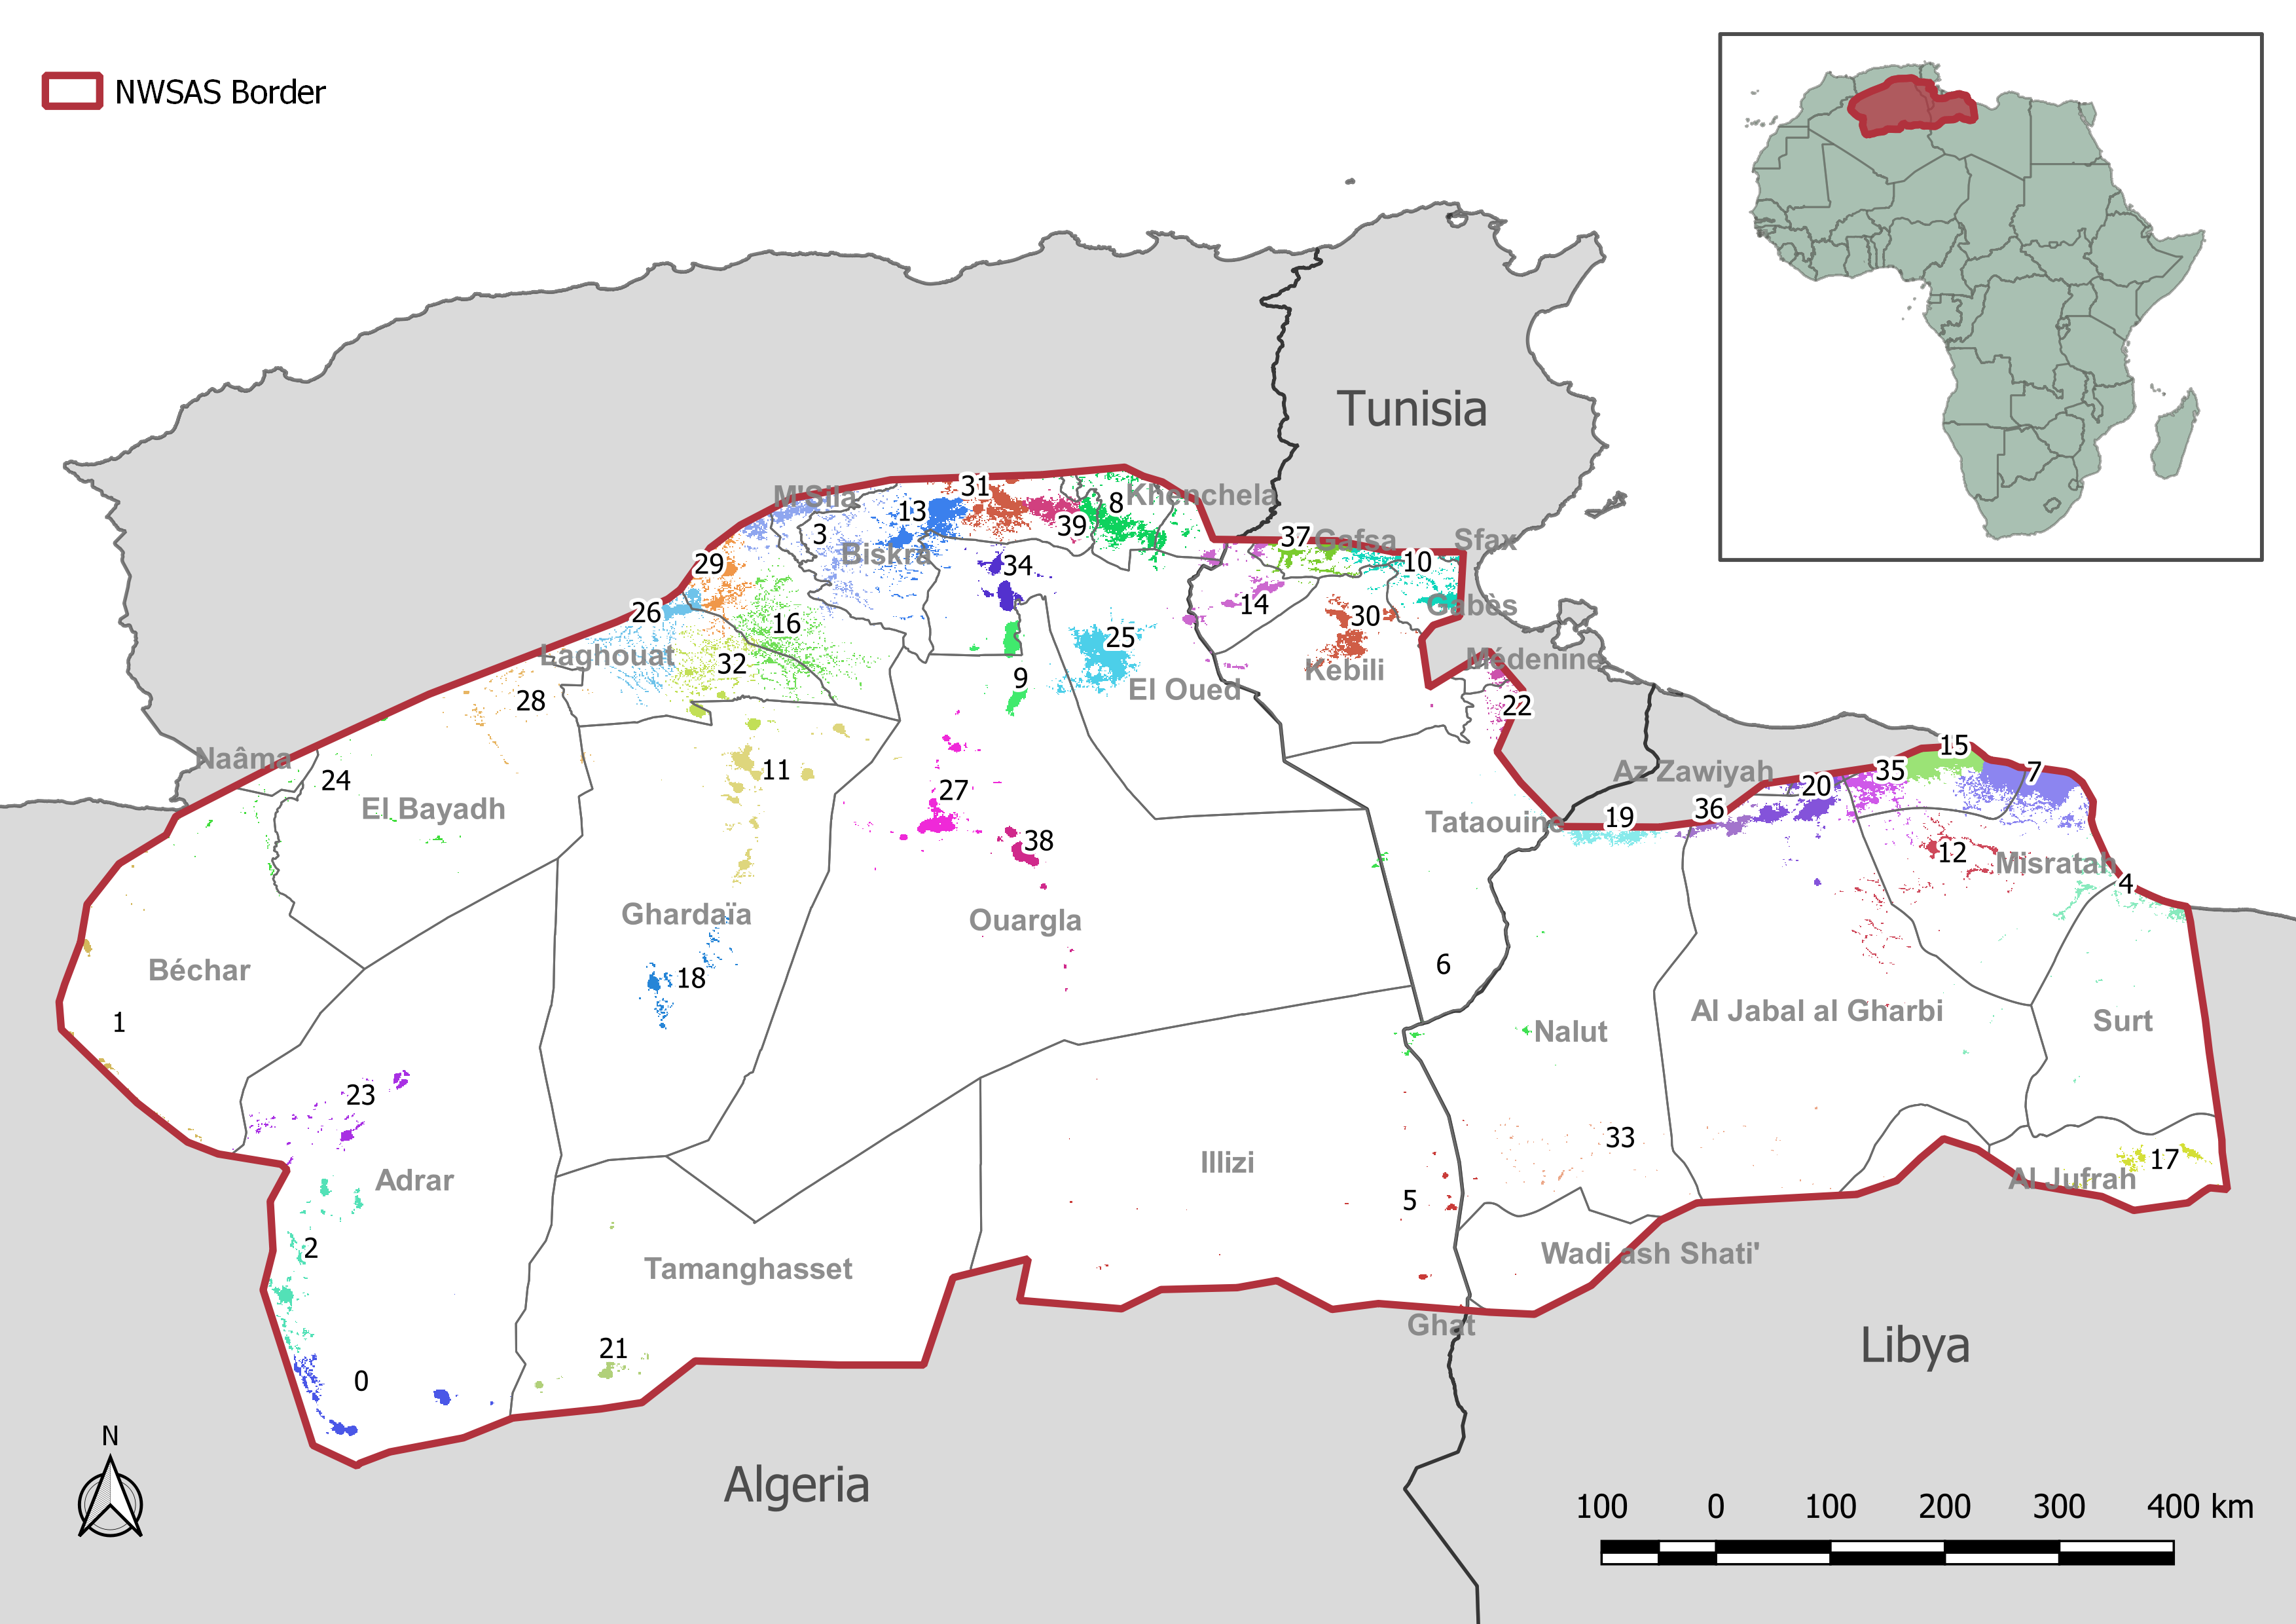
\includegraphics[width=\textwidth, cfbox=black 1pt 0pt]{NWSAS_clusters}
	\caption{Population and cropland clusters. Clusters are numbered from 0 to 39, yielding 40 agglomerations including each population and cropland areas. Every cluster is tagged with a number and colored to make them stand out from others. The grey administrative boundaries correspond to the different provinces.}
	\label{fig:clusters}
\end{figure} 

Clusters are numbered from 0 to 39, yielding 40 agglomerations including each population and cropland areas. Every cluster is tagged with a number and colored to make them stand out from others.


\clearpage
\section{Water withdrawals and reuse per cluster}
Additional results on water withdrawals and reuse per cluster, are reported in this section. \Tref{tbl:resultswater}, shows an overview of the total widthawals per scenario, whereas figures 8 to 12 present detailed per cluster results.
\begin{table}[!ht]
	\caption{\label{tbl:resultswater}Summary of water results by scenario. Values calculated for the entire aquifer (total), as well as the minimum (min), maximum (max), average (mean) and median values between the clusters.}
	\footnotesize
	\lineup
	\begin{tabular*}{\textwidth}{@{}*{7}{l}}
		\br
		&        & \centre{5}{Scenario} \\
		\ns
		&        & \crule{5} \\
		Parameter & Value  &  Baseline &  Scenario 1 &  Scenario 2 &  Scenario 3 &  Scenario 4 \\
		\mr
		Water withdrawals (MCM) & total &    4141.7 &      2342.6 &      2244.6 &      2388.4 &      3958.1 \\
		& min &       0.6 &         0.6 &         0.6 &         0.6 &         0.6 \\
		& max &     502.6 &       284.2 &       284.2 &       284.9 &       494.3 \\
		& mean &     103.5 &        58.6 &        56.1 &        59.7 &        99.0 \\
		& median &      49.1 &        23.6 &        23.6 &        25.5 &        44.7 \\
		Water reused (MCM) & total &    0 &      1669.3 &      1022.1 &      2264.0 &      2385.0 \\
		& min &       0.0 &         0.0 &         0.0 &         0.0 &         0.0 \\
		& max &     0 &       212.4 &       119.1 &       296.5 &       304.4 \\
		& mean &      0 &        41.7 &        25.6 &        56.6 &        59.6 \\
		& median &      0 &        15.7 &        13.2 &        28.1 &        29.3 \\
		Water savings (MCM) & total &       0.0 &      1799.1 &      1897.2 &      1753.4 &       183.7 \\
		& min &       0.0 &         0.0 &         0.0 &         0.0 &       -27.1 \\
		& max &       0.0 &       218.5 &       225.0 &       217.7 &        66.7 \\
		& mean &       0.0 &        45.0 &        47.4 &        43.8 &         4.6 \\
		& median &       0.0 &        19.0 &        19.5 &        17.1 &         2.9 \\
		\br
	\end{tabular*}
\end{table}


\begin{figure}[!h]
	\centering
	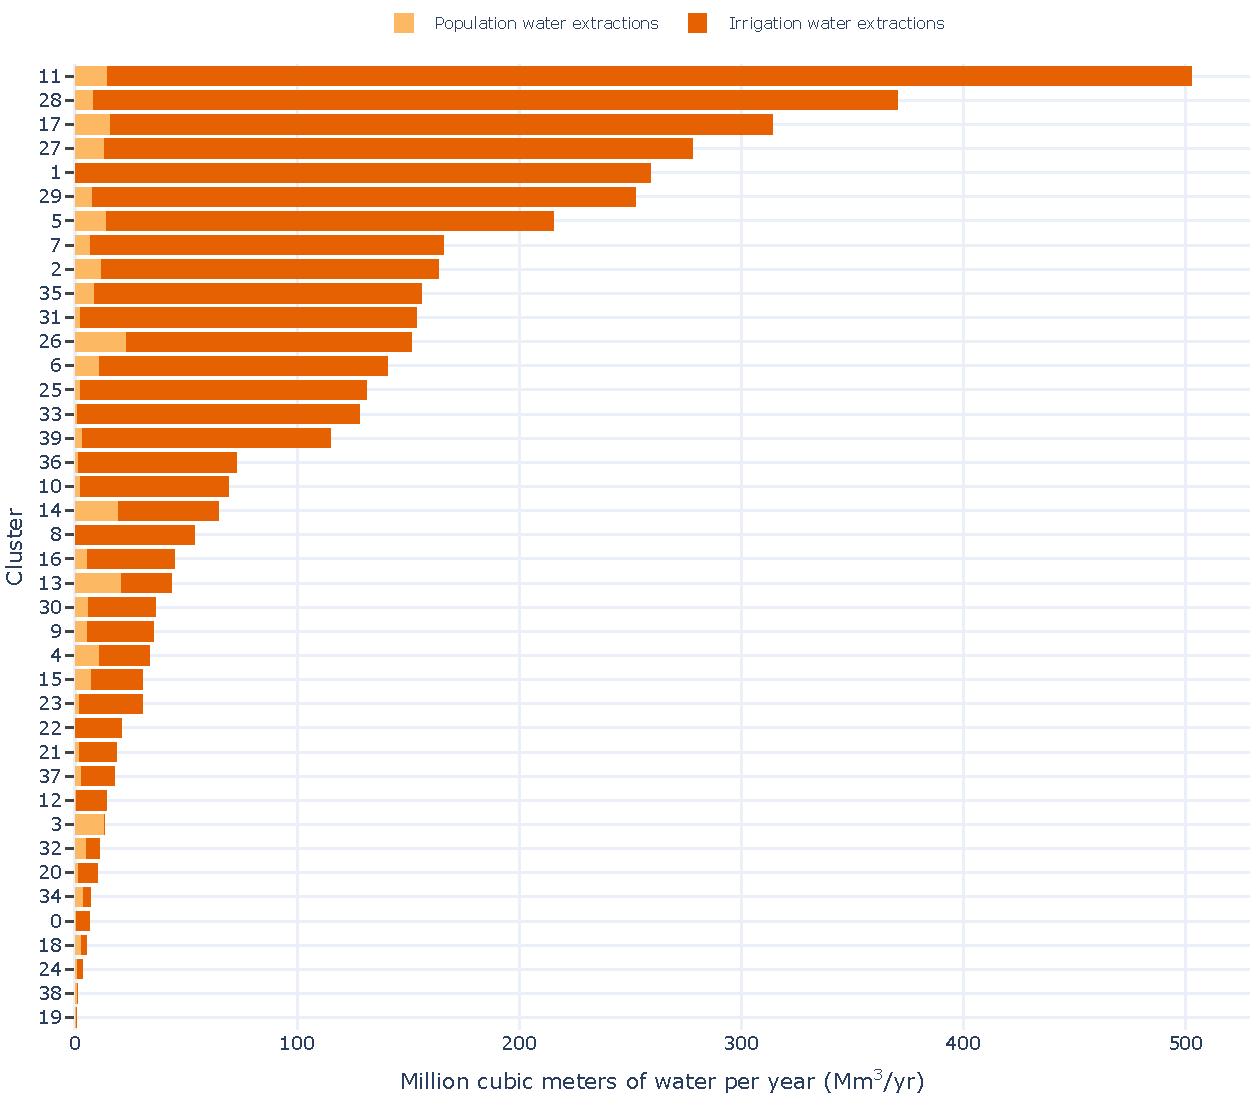
\includegraphics[width=\textwidth]{BaselineWater}
	\caption{Water withdrawals by cluster. Baseline scenario.}
	\label{fig:BaselineWater}
\end{figure}

\begin{figure}[!h]
	\centering
	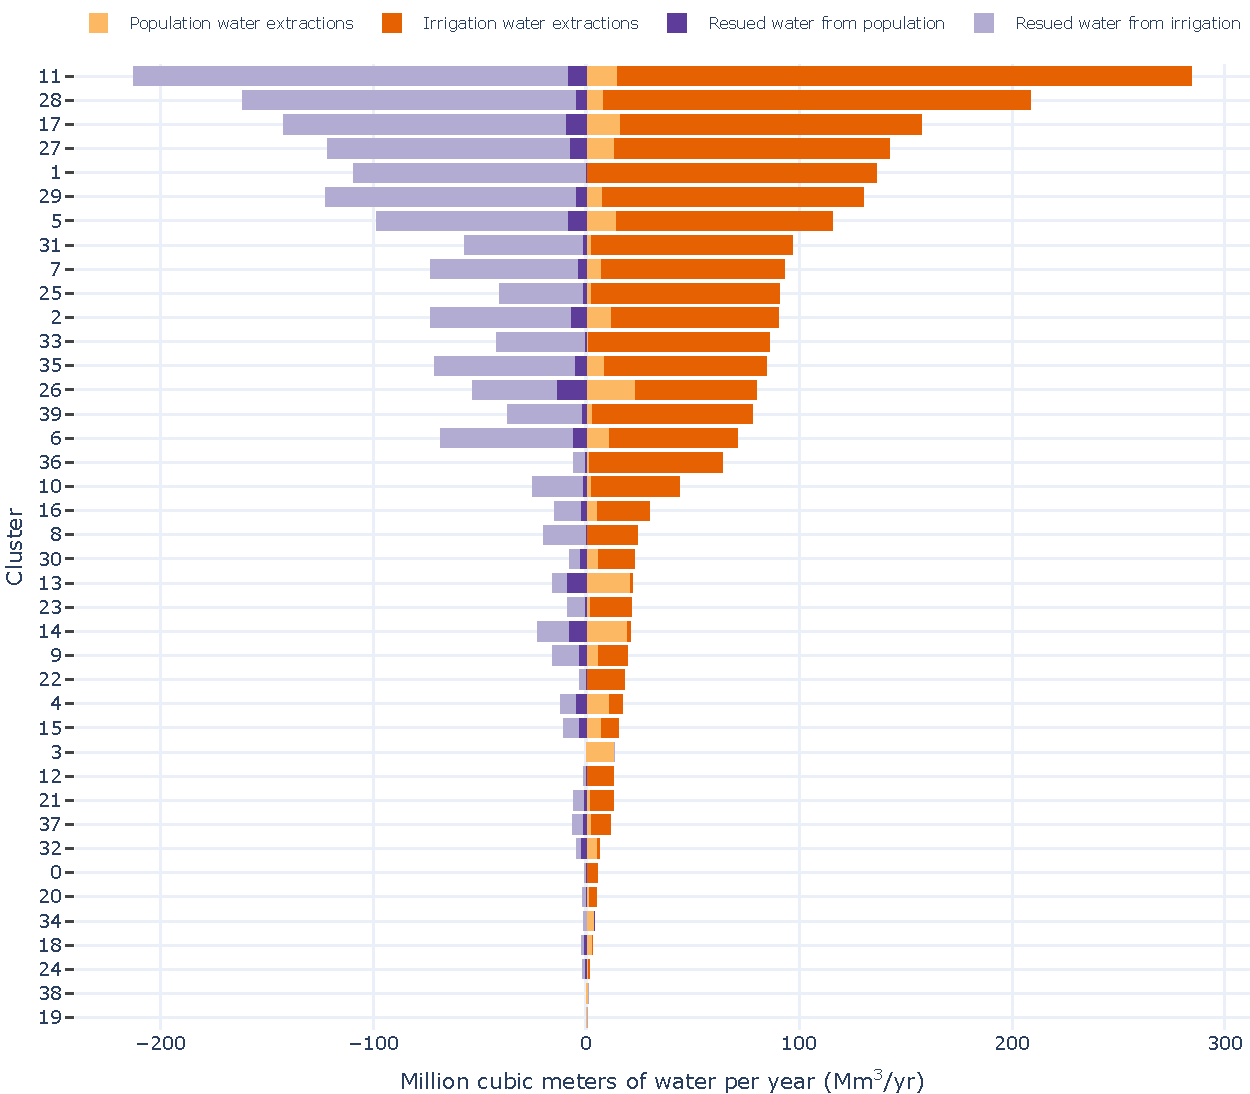
\includegraphics[width=\textwidth]{BaselineWaterWithReuse}
	\caption{Water withdrawals and reuse by cluster. Scenario 1.}
	\label{fig:BaselineWaterReuse}
\end{figure}

\begin{figure}[!h]
	\centering
	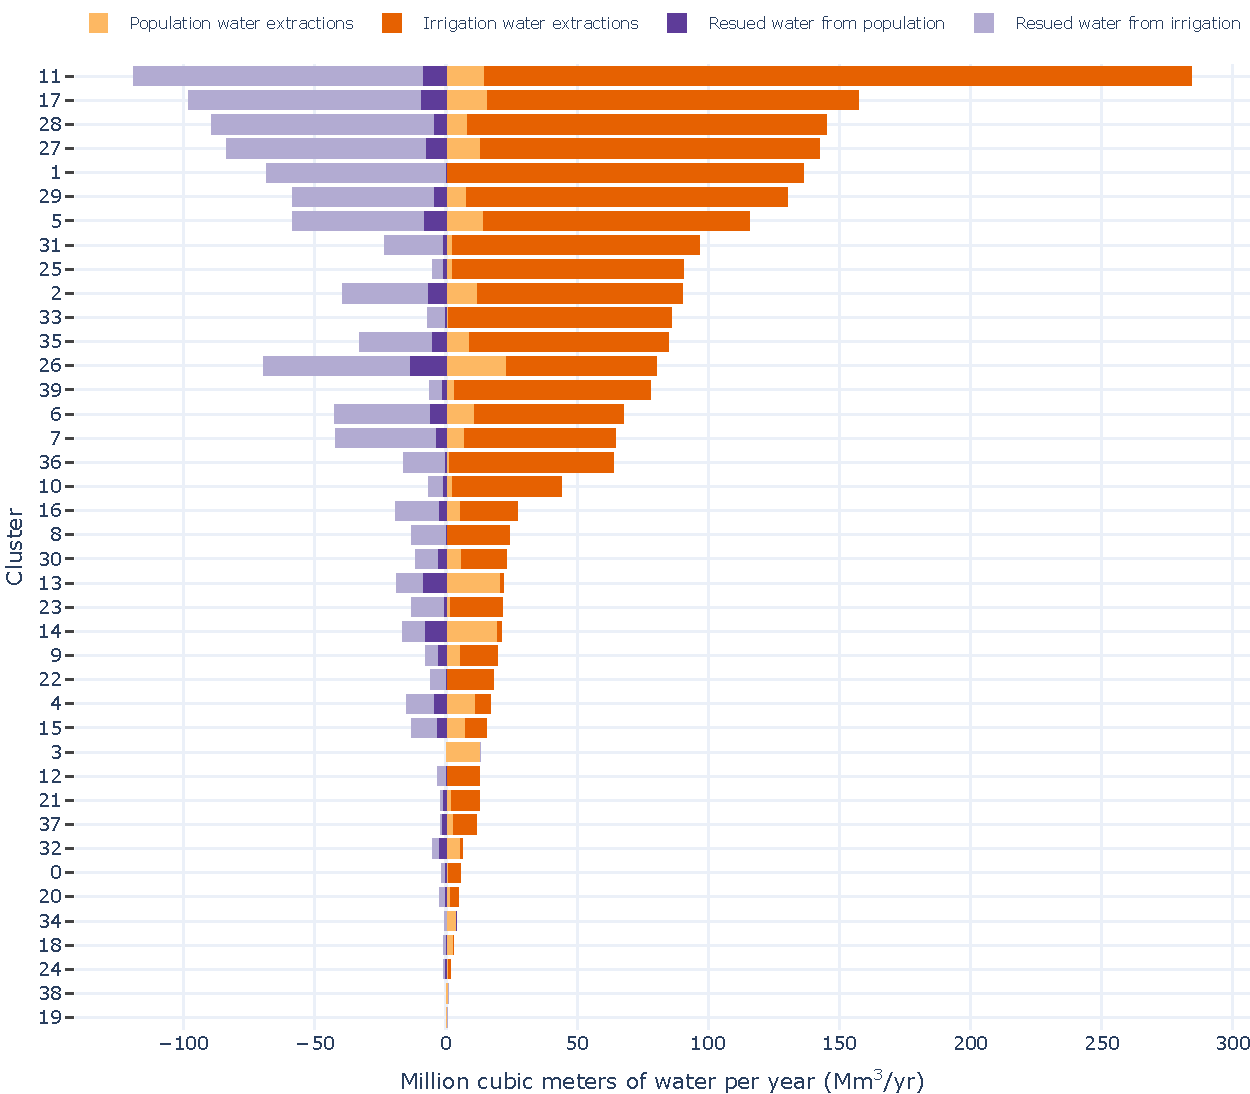
\includegraphics[width=\textwidth]{Scenario2Water}
	\caption{Water withdrawals and reuse by cluster. Scenario 2.}
	\label{fig:Scenario2Water}
\end{figure}

\begin{figure}[!h]
	\centering
	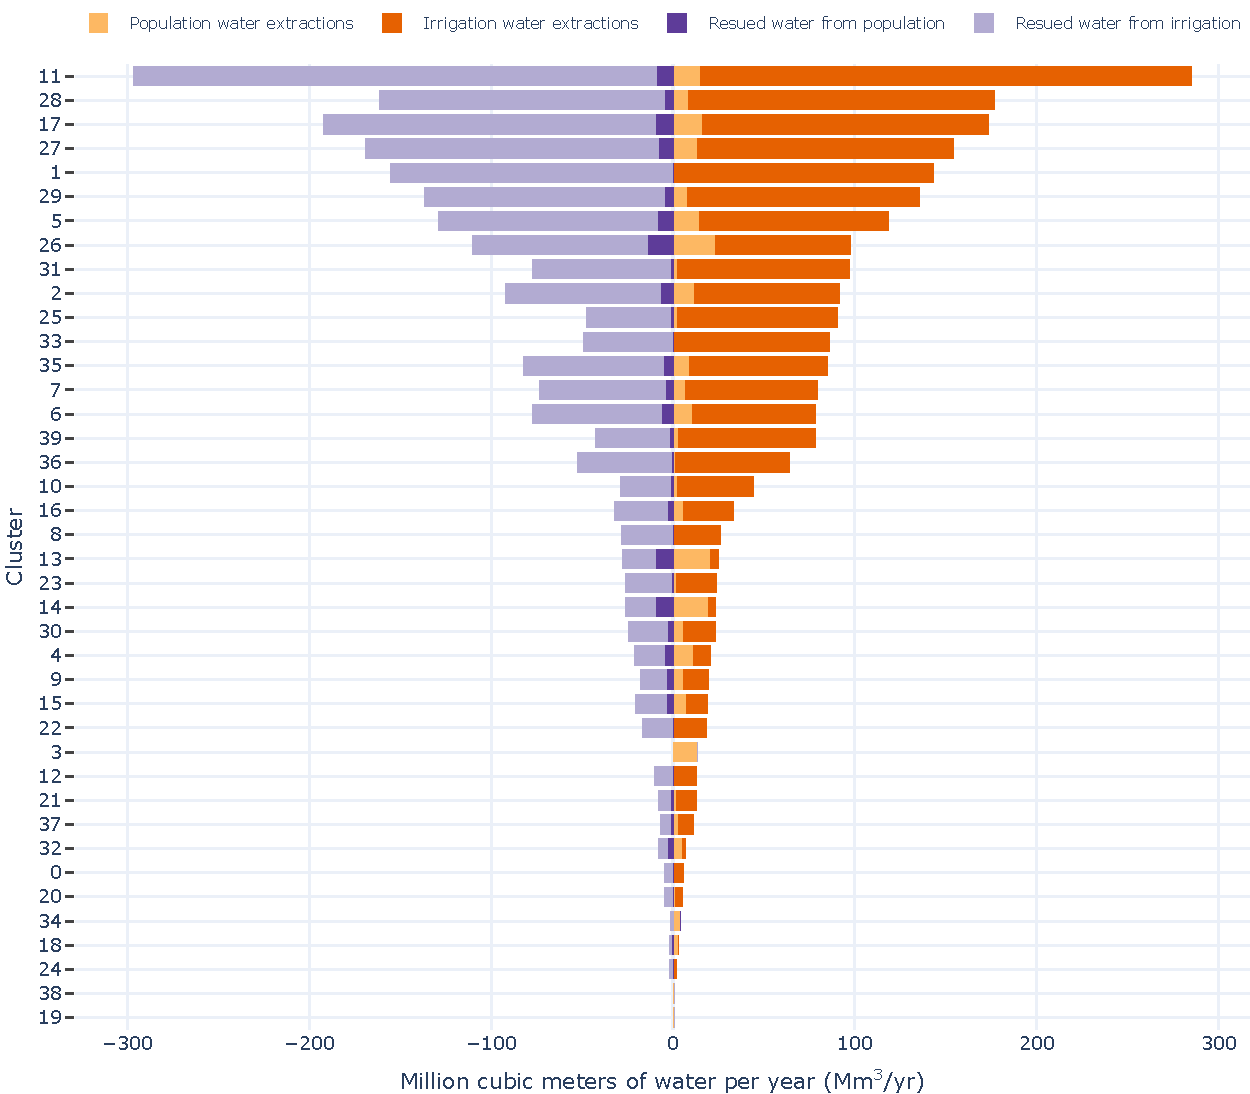
\includegraphics[width=\textwidth]{Scenario3Water}
	\caption{Water withdrawals and reuse by cluster. Scenario 3.}
	\label{fig:Scenario3Water}
\end{figure}

\begin{figure}[!h]
	\centering
	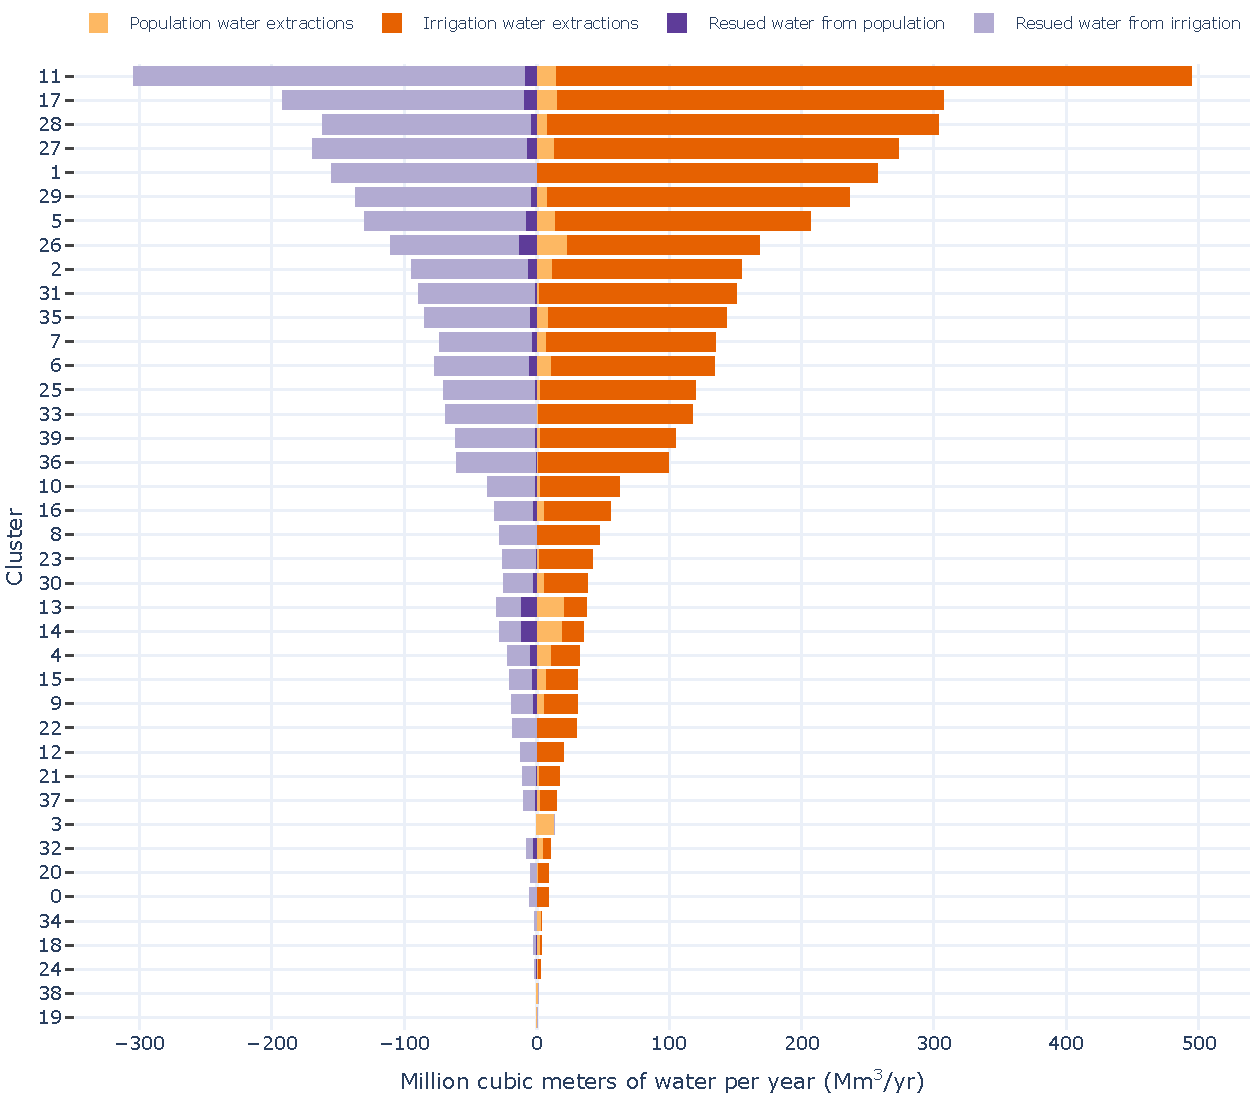
\includegraphics[width=\textwidth]{Scenario4Water}
	\caption{Water withdrawals and reuse by cluster. Scenario 4.}
	\label{fig:Scenario4Water}
\end{figure}

\clearpage
\section{Energy demand per cluster}
In this section, additional results concerning the energy requirements for water pumping, water desalination and wastewater treatment are presented. An overview for each scenario can be found in \tref{tbl:resultsenergy}, presenting total, min, max, mean,and median values. Moreover, figures 13 to 17 show detailed per cluster results.
\begin{table}[!ht]
	\caption{\label{tbl:resultsenergy}Summary of results by scenario. Selected results are calculated for the entire aquifer (total), as well as the minimum (min), maximum (max), average (mean) and median values between the clusters.}
	\footnotesize
	\lineup
	\begin{tabular*}{\textwidth}{@{}*{7}{l}}
		\br
		&        & \centre{5}{Scenario} \\
		\ns
		&        & \crule{5} \\
		Parameter & Value  &  Baseline &  Scenario 1 &  Scenario 2 &  Scenario 3 &  Scenario 4 \\
		\mr
		Energy (GWh) & total &    3055.7 &      2153.3 &      2005.0 &      2223.6 &      3515.9 \\
		& min &       0.5 &         0.6 &         0.6 &         0.6 &         0.6 \\
		& max &     402.8 &       288.5 &       274.0 &       302.1 &       491.3 \\
		& mean &      76.4 &        53.8 &        50.1 &        55.6 &        87.9 \\
		& median &      26.7 &        19.9 &        19.8 &        21.6 &        34.1 \\
		\br
	\end{tabular*}
\end{table}

\begin{figure}[!h]
	\centering
	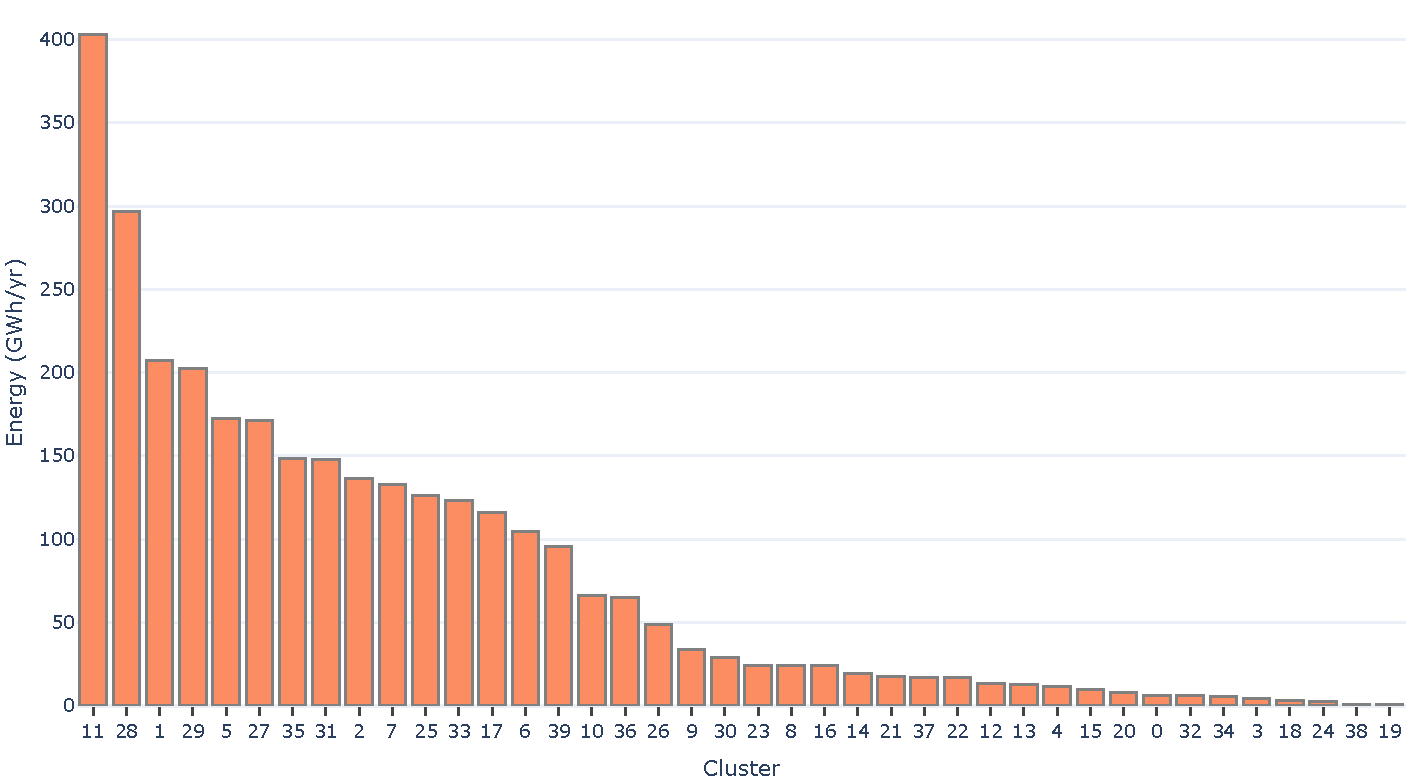
\includegraphics[width=\textwidth]{BaselineEnergy}
	\caption{Energy requirements per cluster for pumping in the Baseline scenario.}
	\label{fig:BaselineEnergy}
\end{figure}

\begin{figure}[!h]
	\centering
	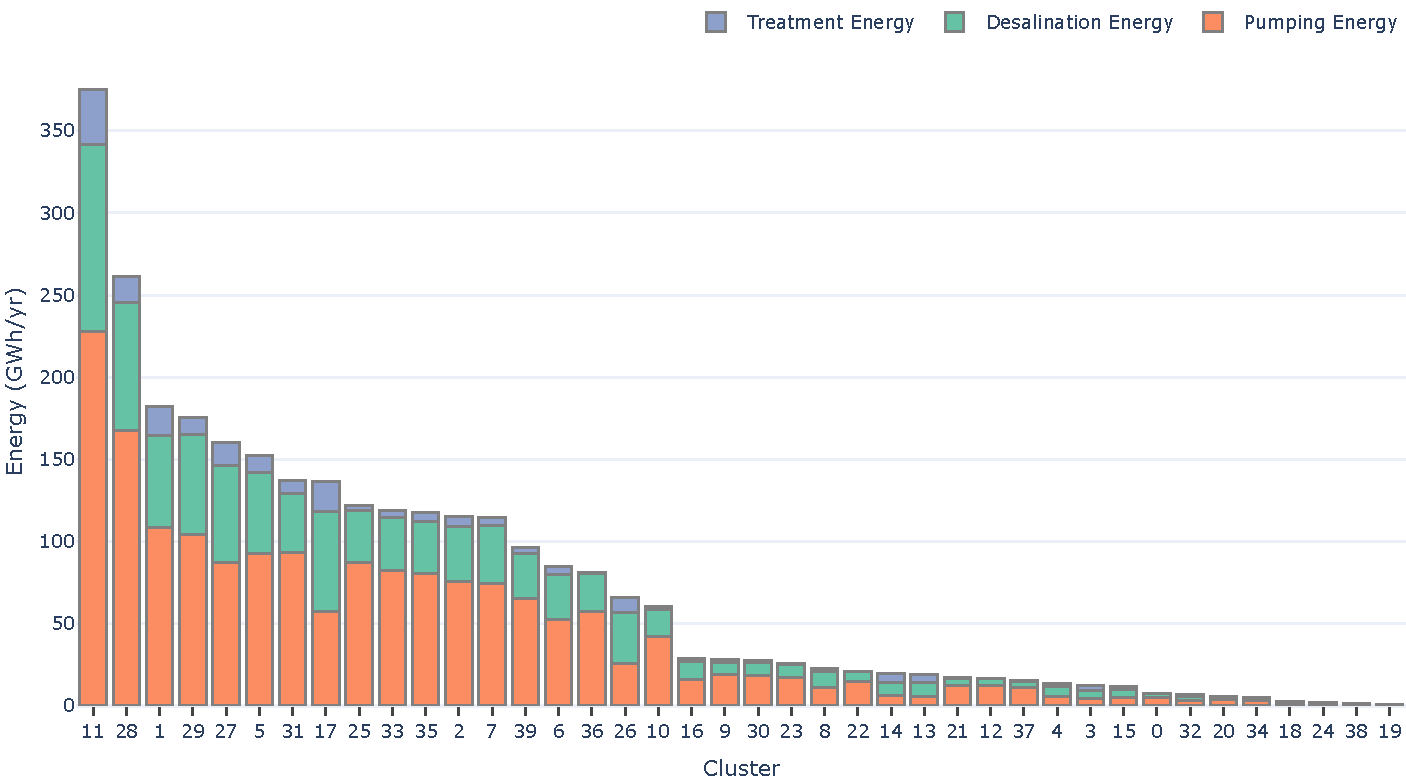
\includegraphics[width=\textwidth]{Scenario1Energy}
	\caption{Energy requirements per cluster for pumping in Scenario 1.}
	\label{fig:Scenario1Energy}
\end{figure}

\begin{figure}[!h]
	\centering
	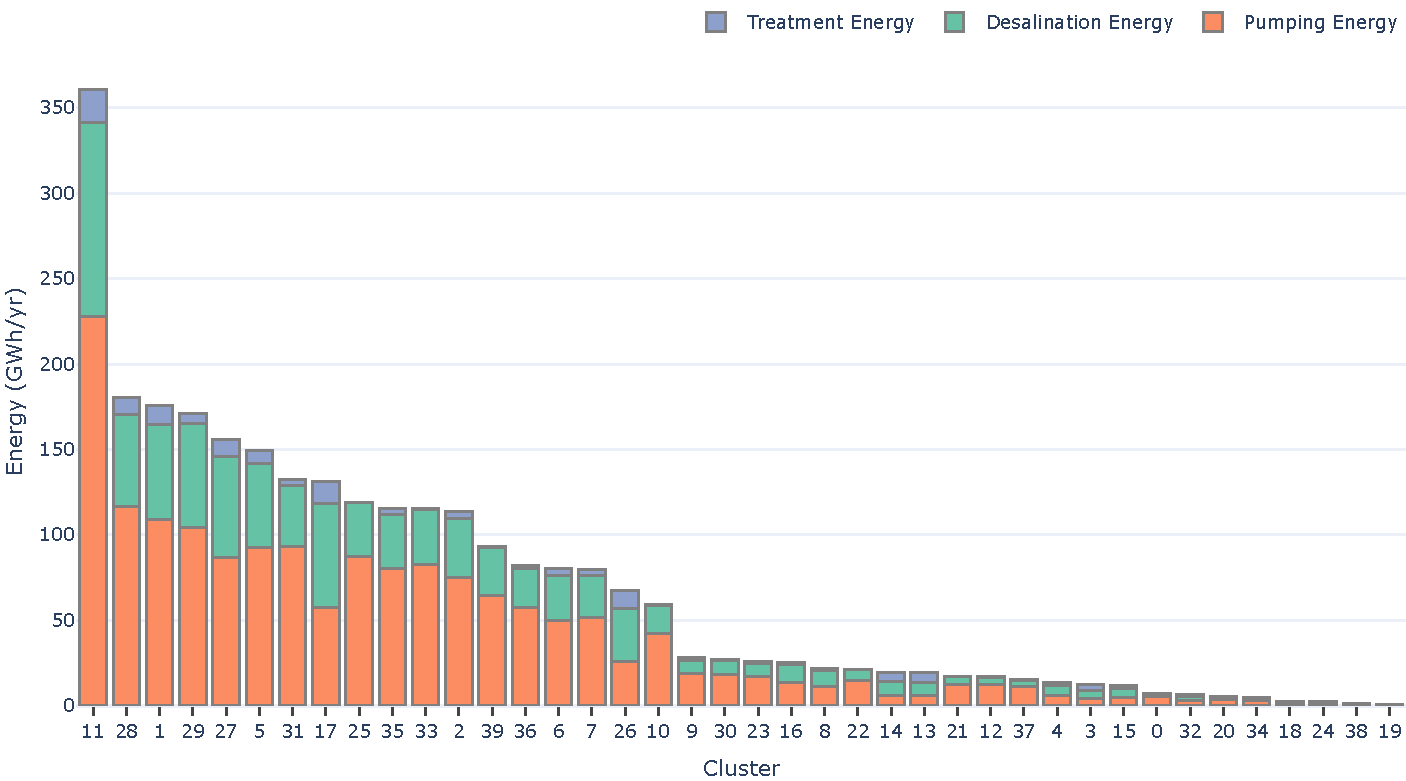
\includegraphics[width=\textwidth]{Scenario2Energy}
	\caption{Energy requirements per cluster for pumping in Scenario 2.}
	\label{fig:Scenario2Energy}
\end{figure}

\begin{figure}[!h]
	\centering
	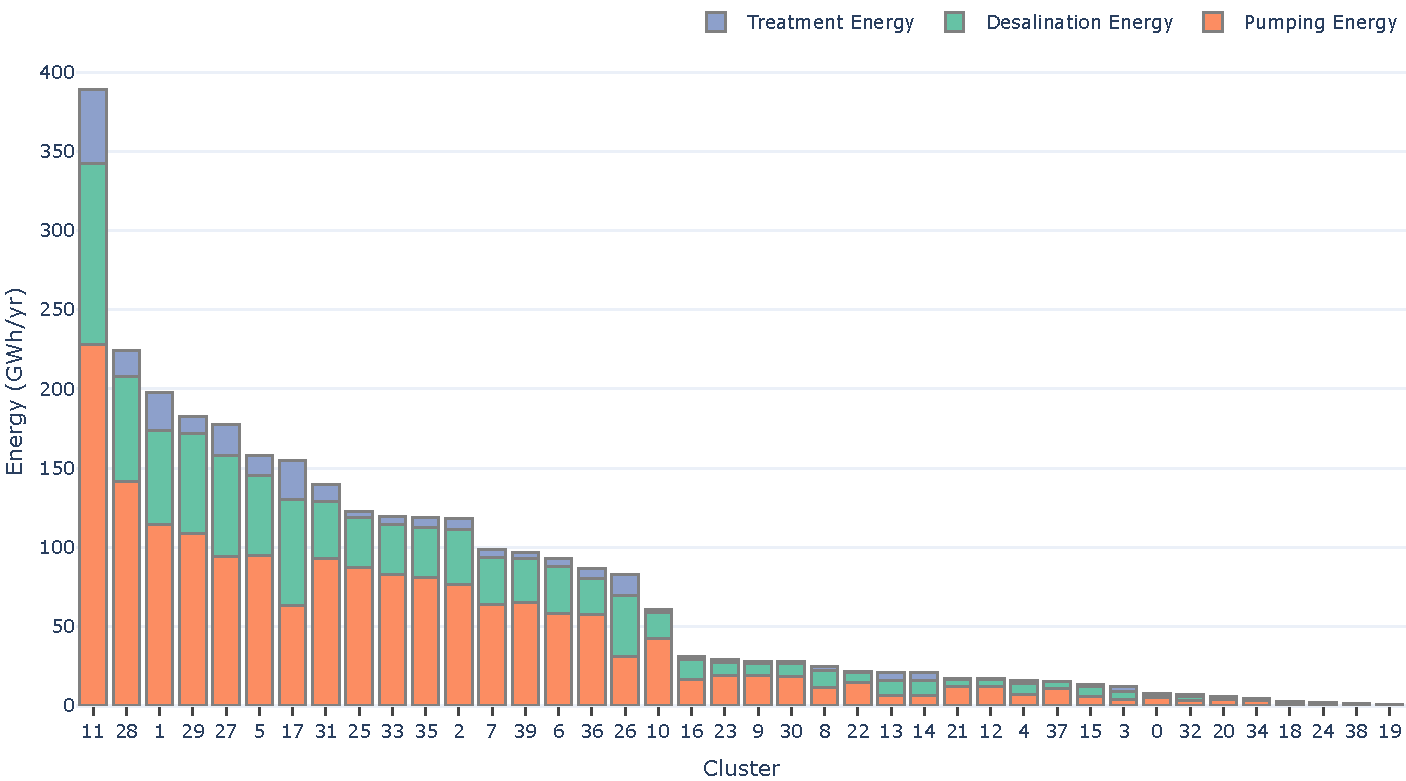
\includegraphics[width=\textwidth]{Scenario3Energy}
	\caption{Energy requirements per cluster for pumping in Scenario 3.}
	\label{fig:Scenario3Energy}
\end{figure}

\begin{figure}[!h]
	\centering
	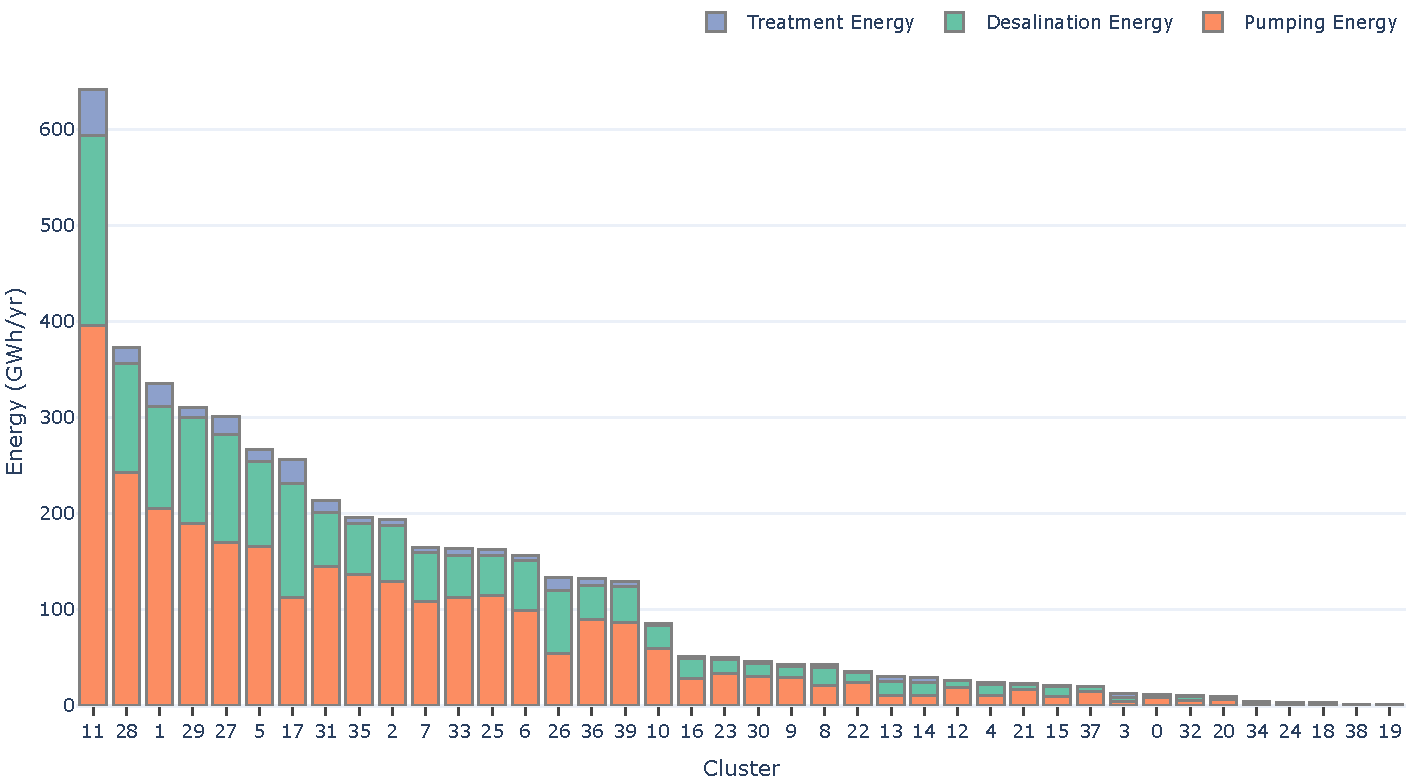
\includegraphics[width=\textwidth]{Scenario4Energy}
	\caption{Energy requirements per cluster for pumping in Scenario 4.}
	\label{fig:Scenario4Energy}
\end{figure}


\clearpage
\section{Least-cost technologies}
This section expands the results on least-cost technologies identified. The least cost options, are highly dependent on the treatment capacity needed, to show this more clearly, a subset of the largest clusters (in terms of water use) is done in \fref{fig:lcowlargestclusters}. from there, it can be seen that the technologies LCOW values can vary largely if water withdrawals (or capacity) changes. Take for example cluster1. It has very large irrigation water extractions, which makes the on-farm pond system to be cheap for tailwater treatment, however, the treatment technology options available for domestic wastewater all have fairly large values. This is due to the low water uses of the domestic sector in this cluster, which is driven by low population near the agricultural areas.

\begin{figure}[!h]
	\centering
	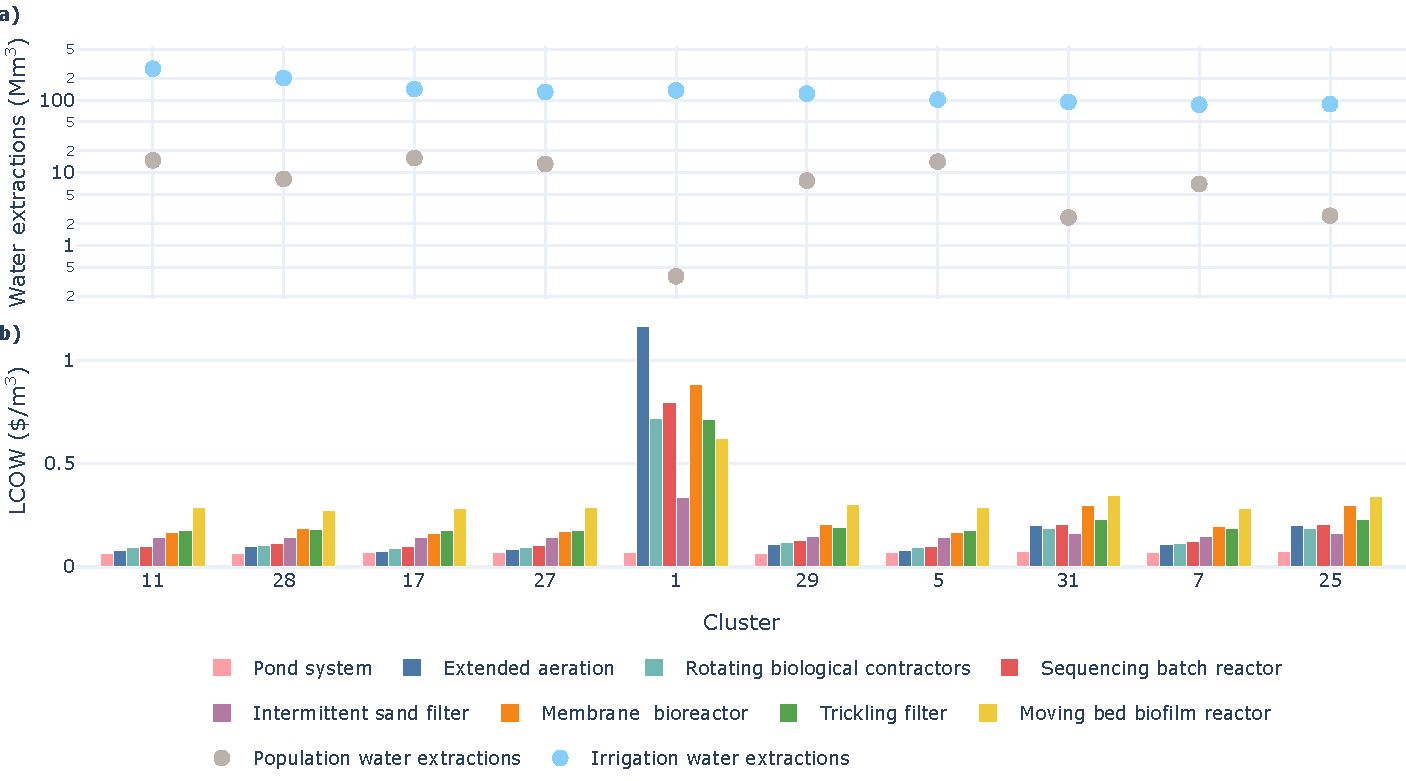
\includegraphics[width=\textwidth]{BaselineLCOW_largest_clusters}
	\caption{Energy requirements for pumping change due to groundwater depth increase. This was calculated for Scenario 1 and all pumping requirements throughout the basin were aggregated}
	\label{fig:lcowlargestclusters}
\end{figure}

Moreover, detailed maps of the technologies chosen for domestic wastewater treatment can be seen in figures 19, 20 and 21, for different domestic water uses. From \fref{fig:leastLowDemand}, it can be seen that with lower water usage, the technology mix is richer throughout the basin, whereas when water use get higher (\fref{fig:leastMidDemand} and \fref{fig:leastHighDemand}) all clusters then to prefer extended aeration. This is due to the economy of scale identified in \fref{fig:lcowlargestclusters}, which shows a trade-off between the least-cost technology and the treatment capacity requirements.

\begin{figure}[!h]
	\centering
	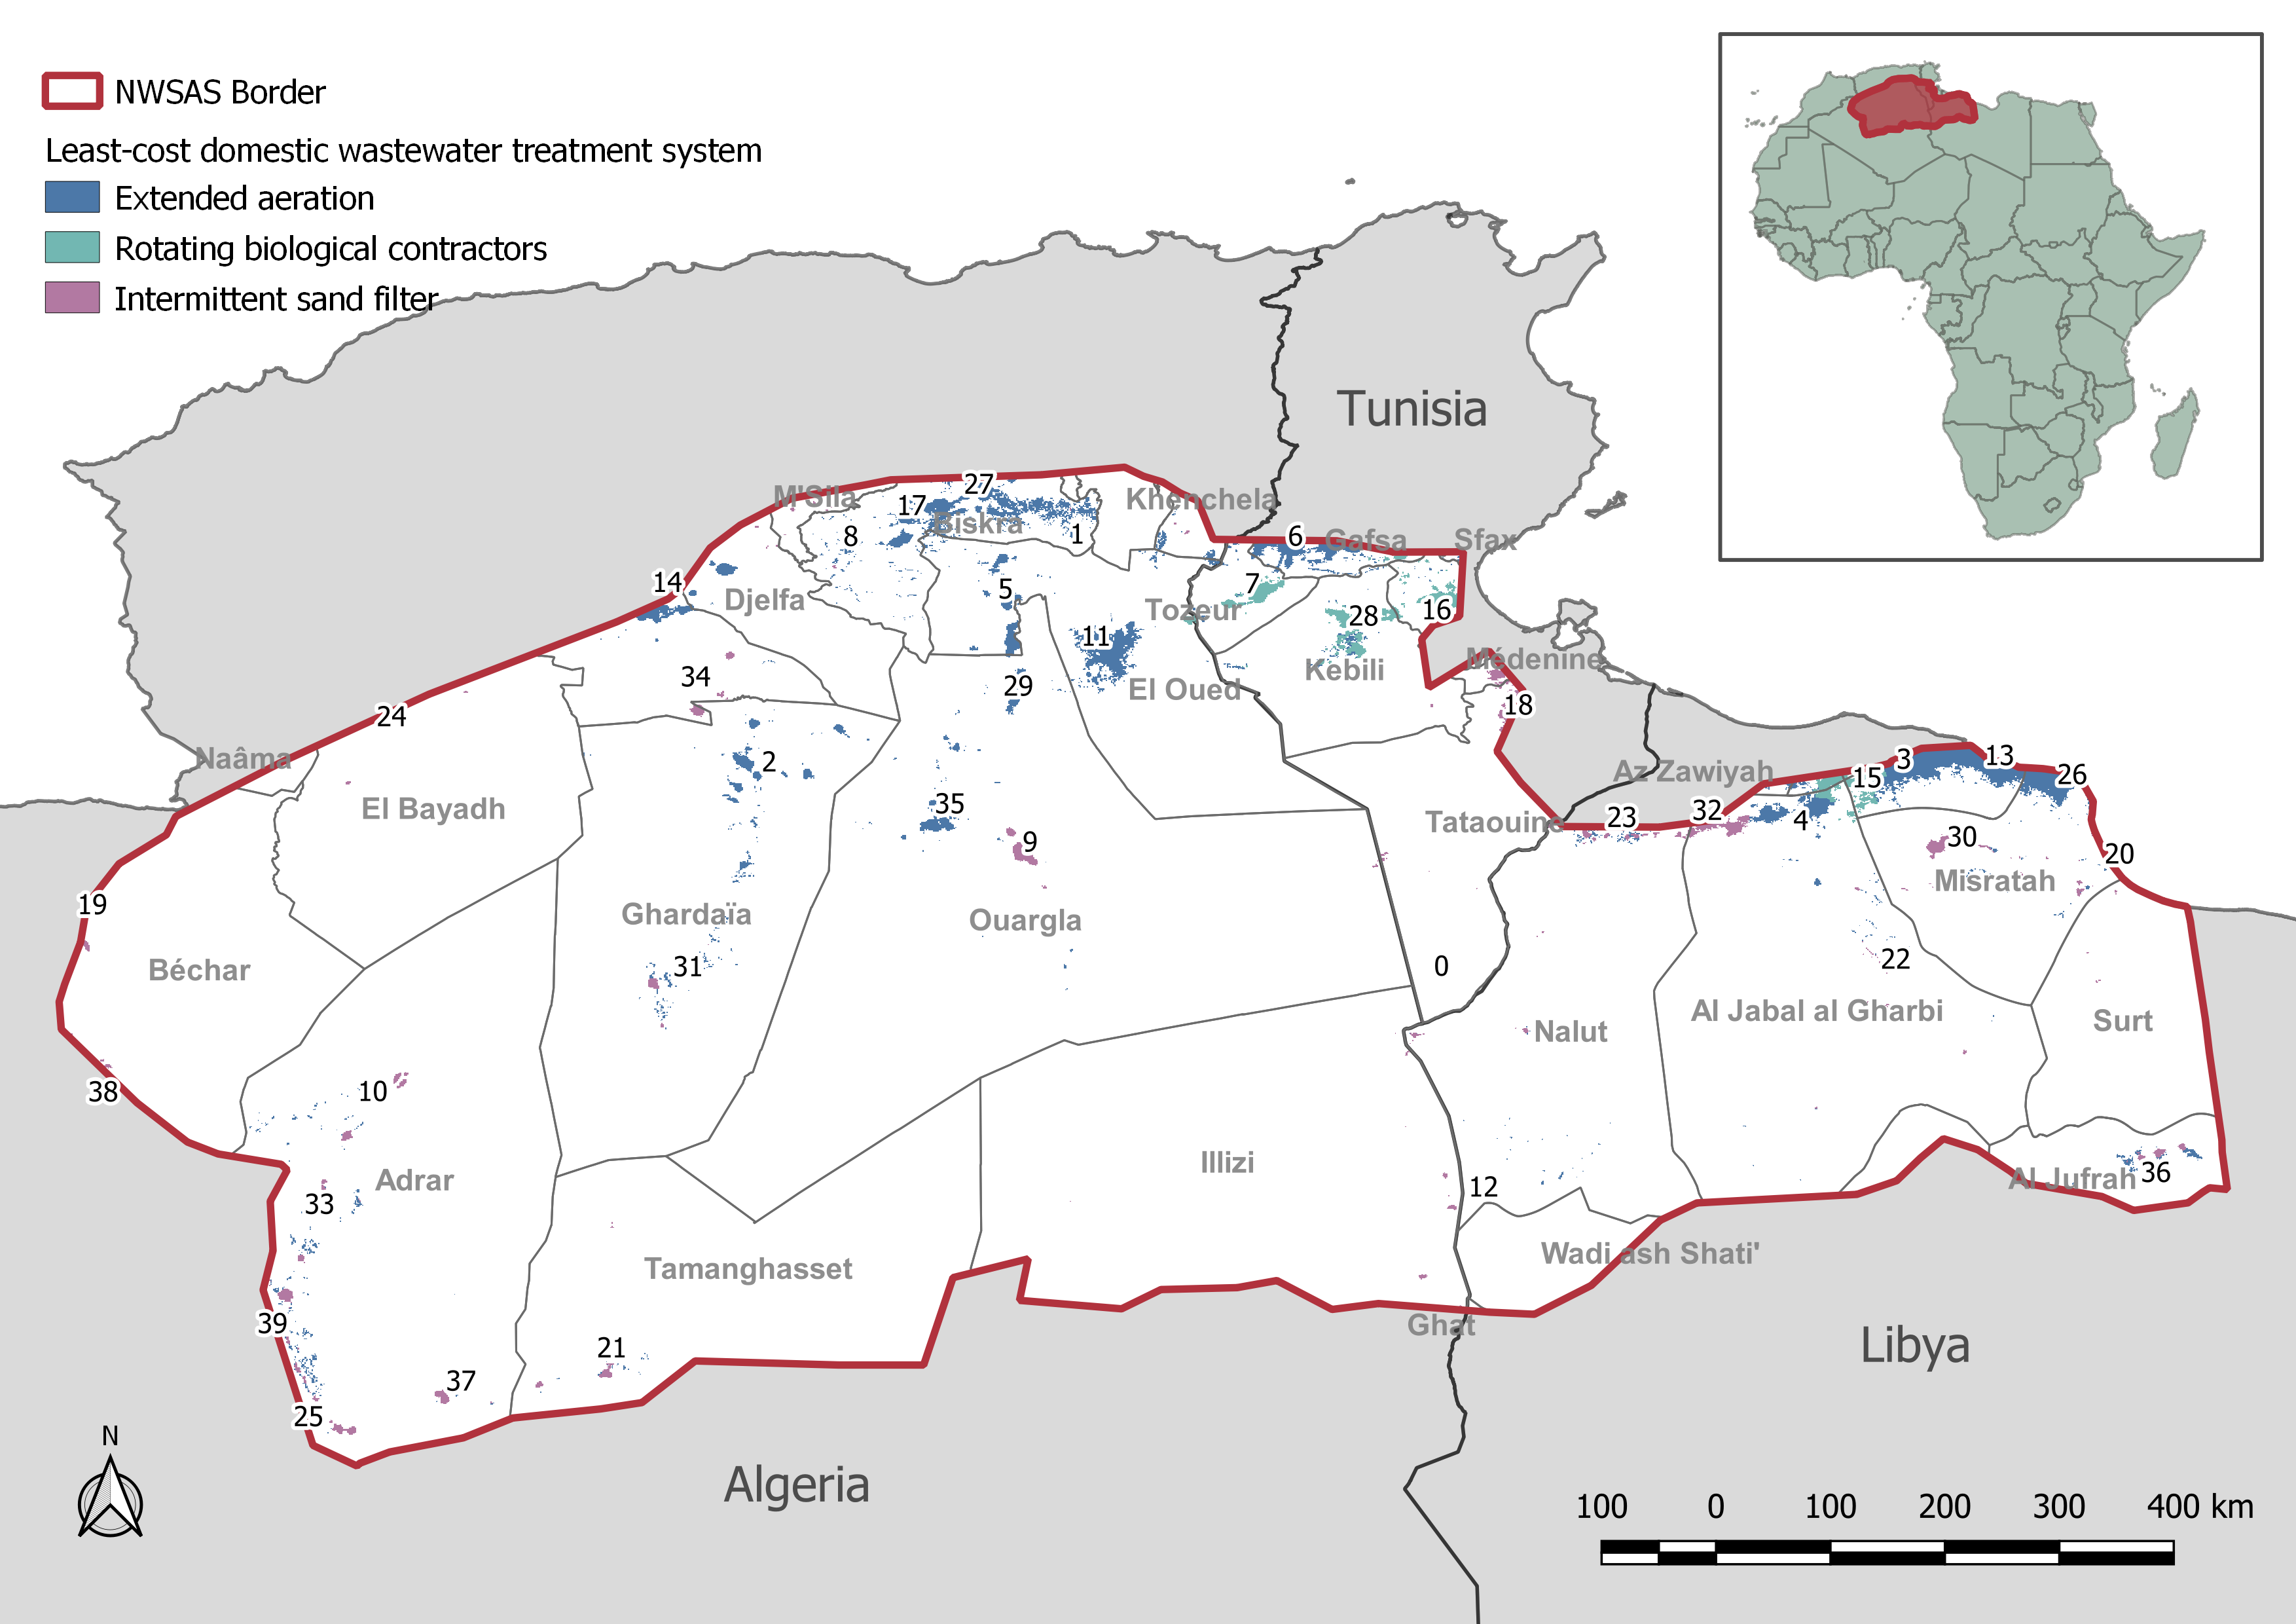
\includegraphics[width=0.9\textwidth, cfbox=black 1pt 0pt]{NWSAS_least_low_demand}
	\caption{Least-cost domestic wastewater treatment system, with low domestic water use (36 m\textsuperscript{3}/yr).}
	\label{fig:leastLowDemand}
\end{figure}

\begin{figure}[!h]
	\centering
	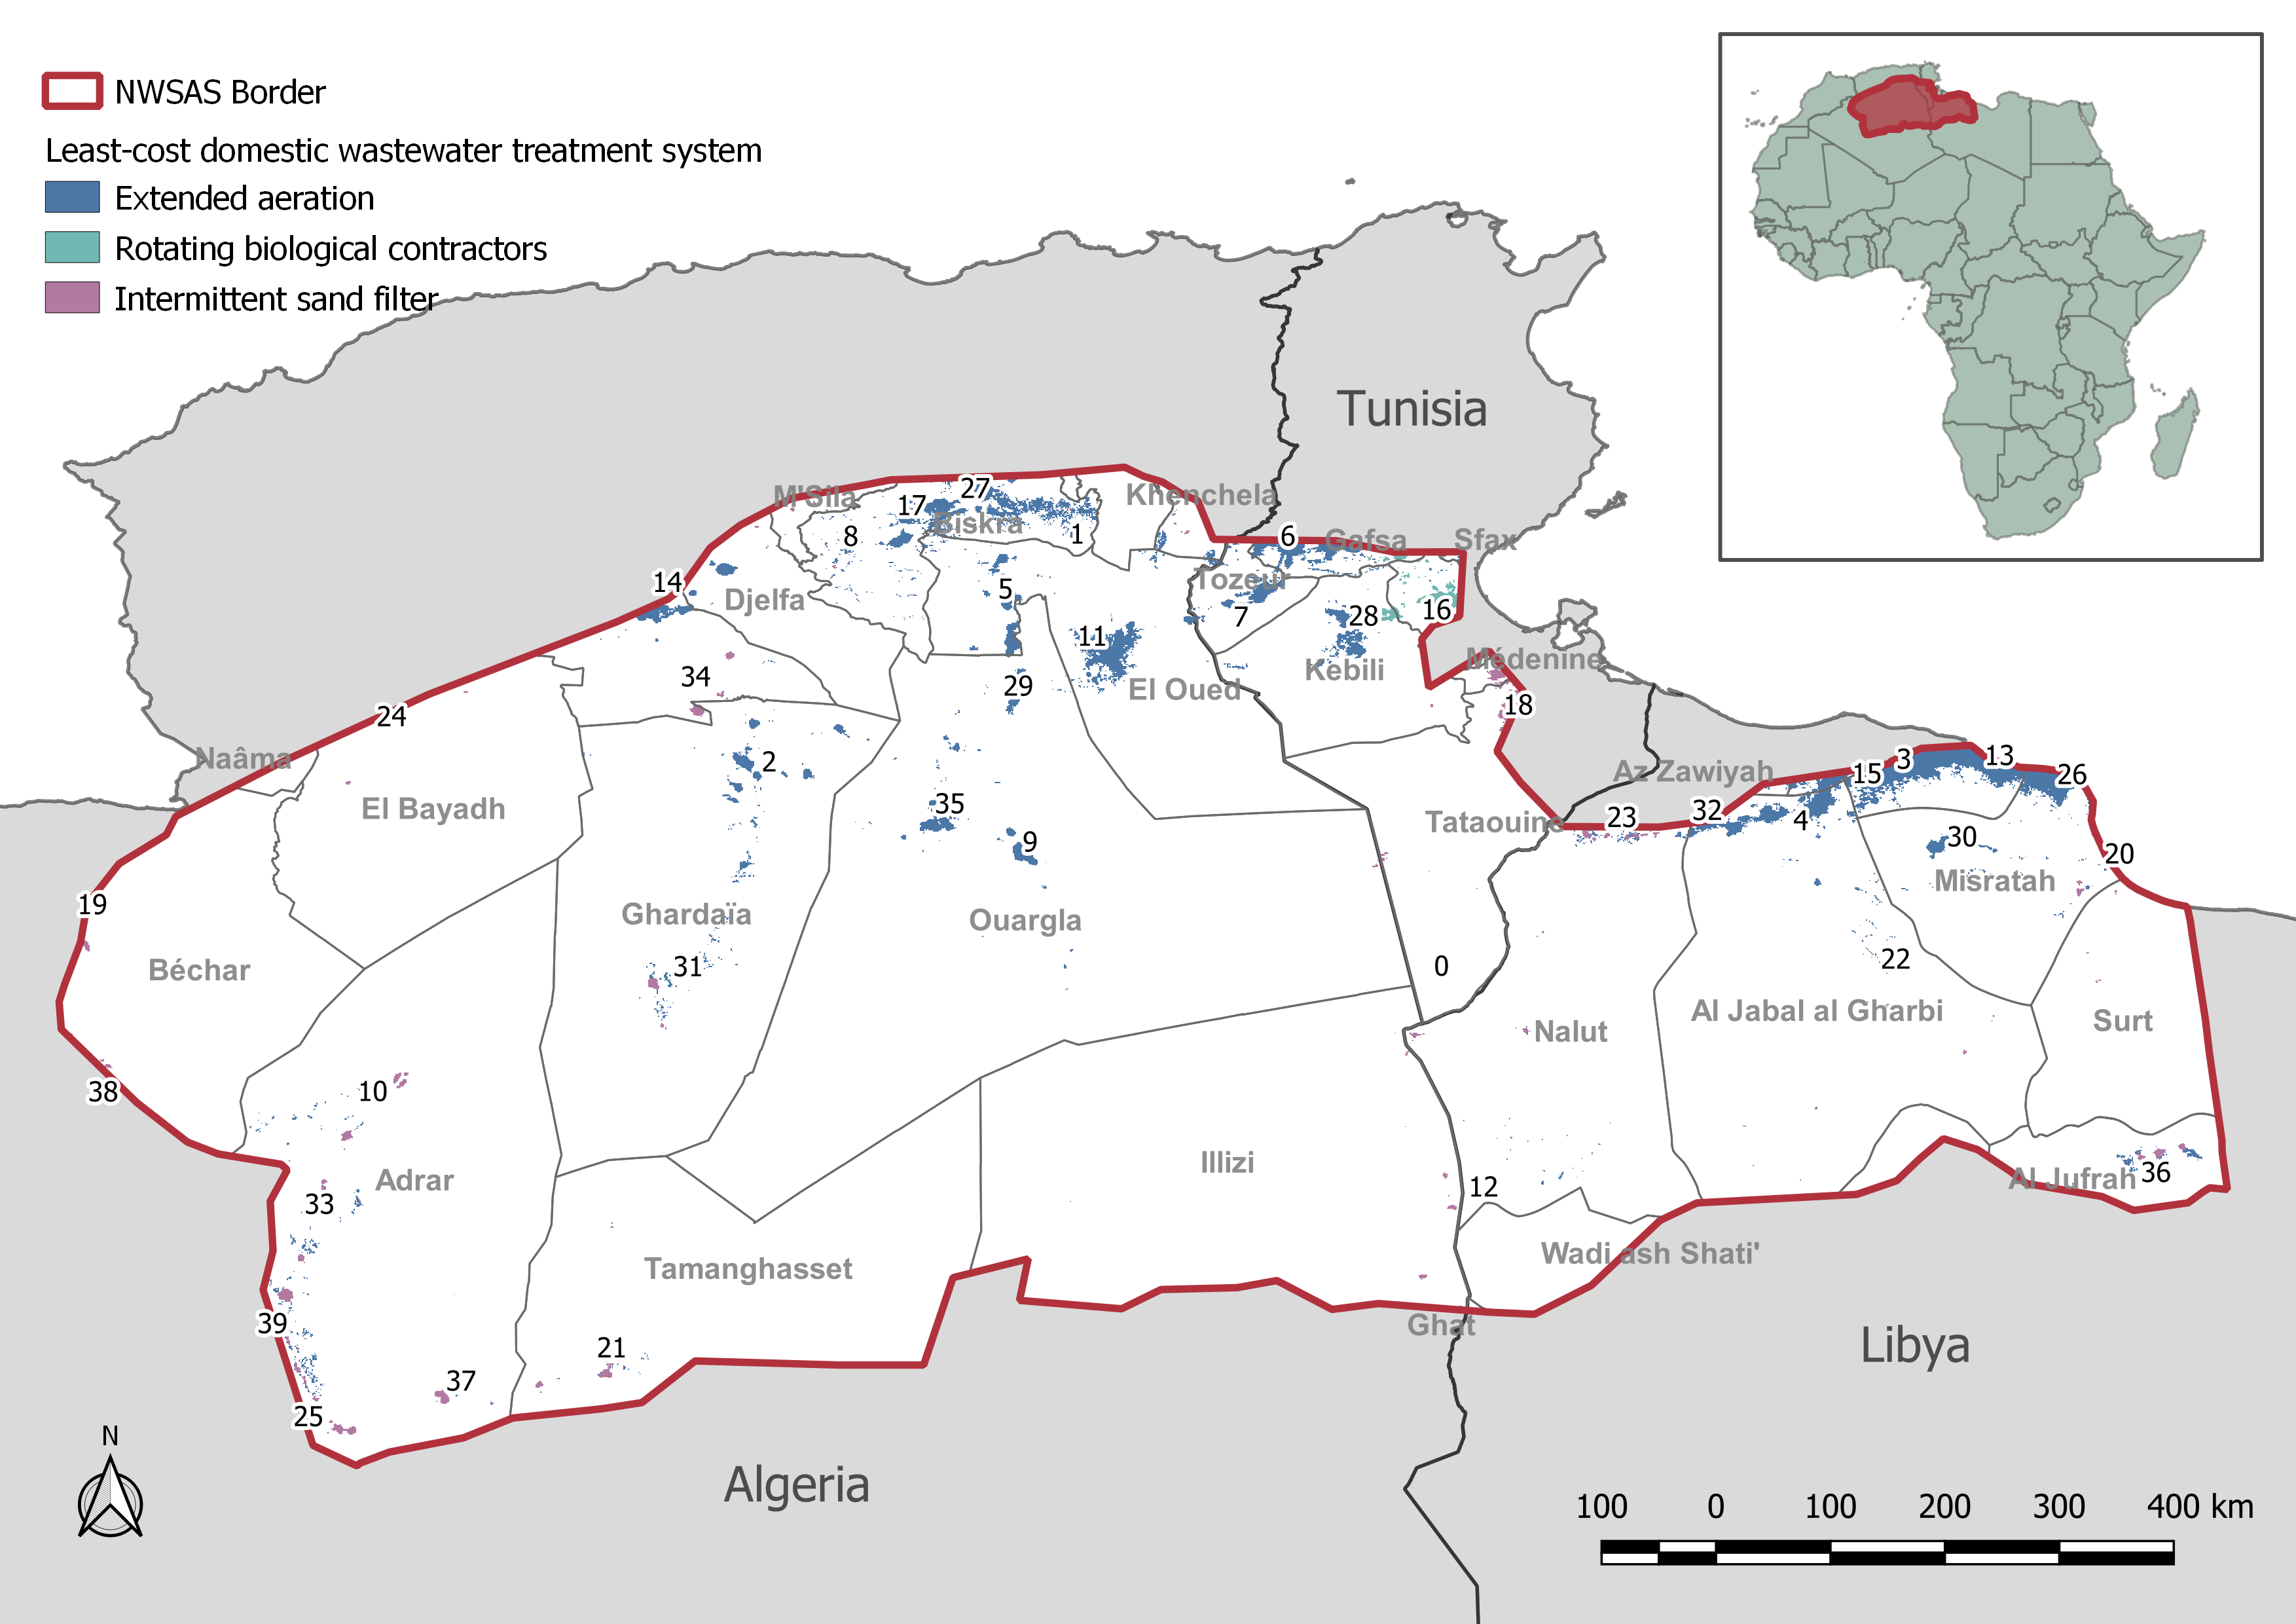
\includegraphics[width=0.9\textwidth, cfbox=black 1pt 0pt]{NWSAS_least_mid_demand}
	\caption{Least-cost domestic wastewater treatment system, with low domestic water use (55 m\textsuperscript{3}/yr).}
	\label{fig:leastMidDemand}
\end{figure}

\begin{figure}[!h]
	\centering
	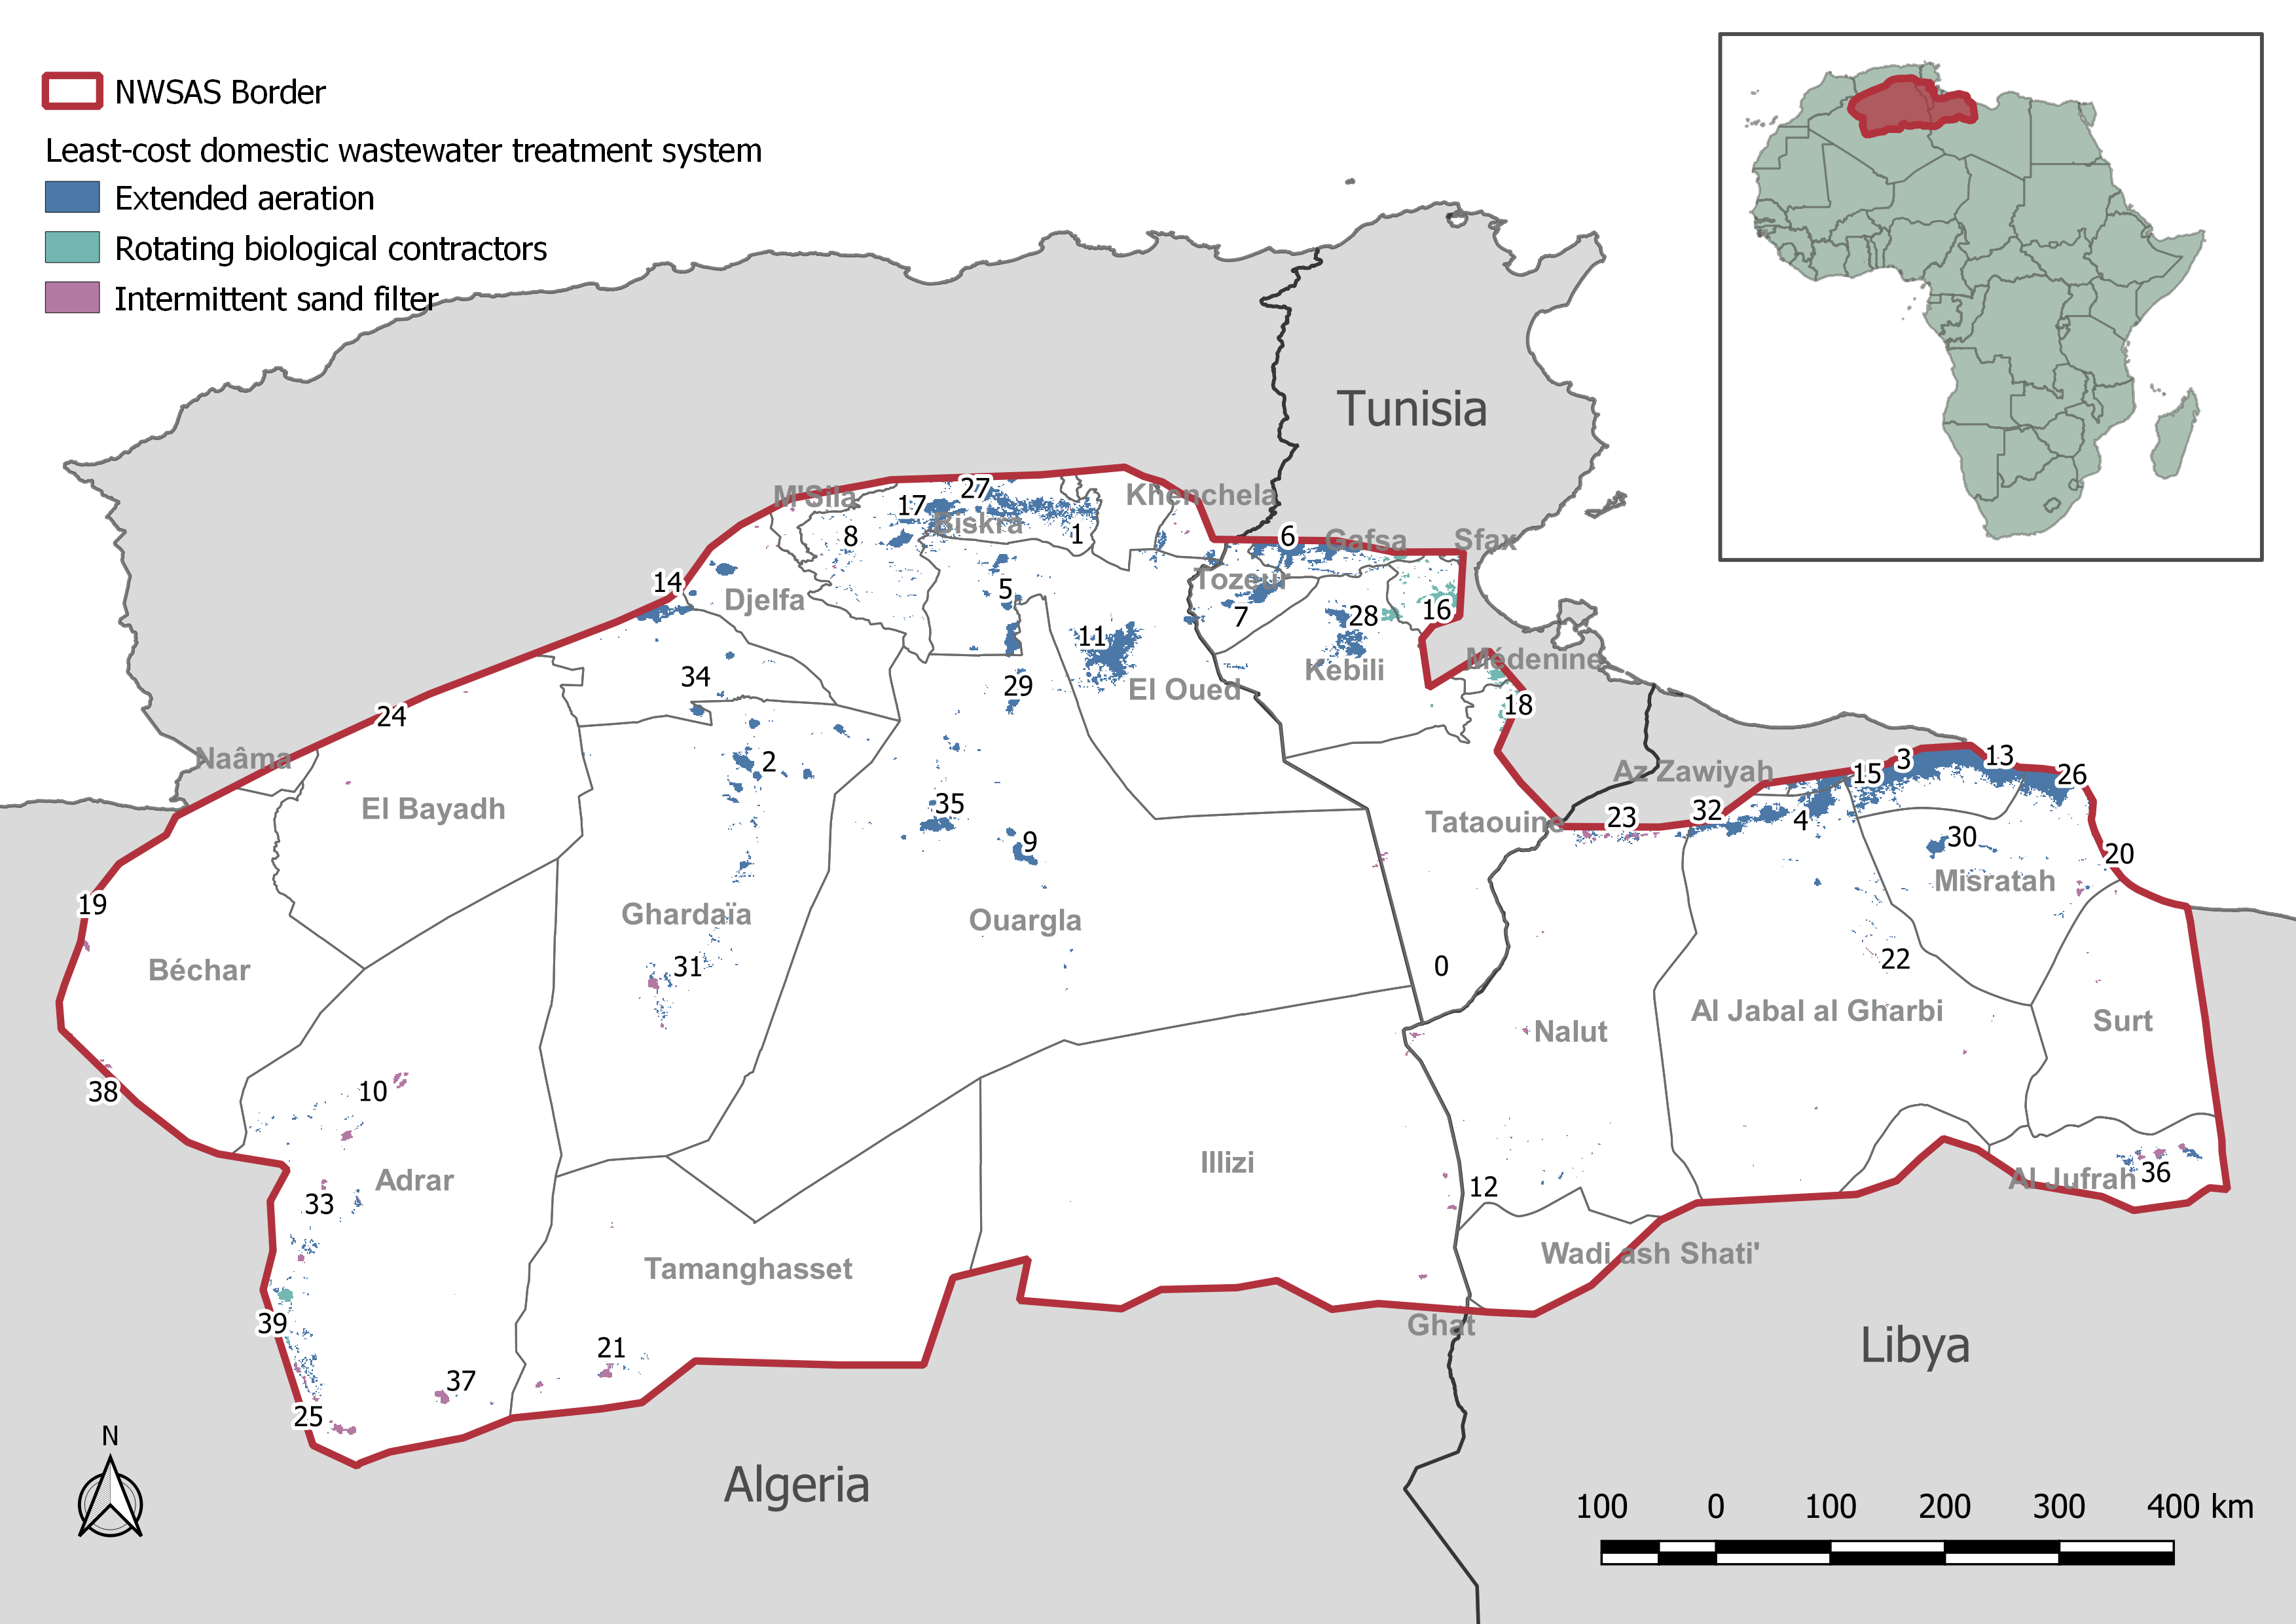
\includegraphics[width=0.9\textwidth, cfbox=black 1pt 0pt]{NWSAS_least_high_demand}
	\caption{Least-cost domestic wastewater treatment system, with low domestic water use (73 m\textsuperscript{3}/yr).}
	\label{fig:leastHighDemand}
\end{figure}


\clearpage
\section{Sensitivity analysis}
Sensitivity analysis were performed on key modeling parameters. This, helps to give clarity on uncertainties associated to the input data. All the sensitivity parameters evaluated are presented in \tref{tbl:sensitivity} and were calculated for Scenario 1 and an average year, unless stated differently.
\begin{table}[!ht]
	\caption{\label{tbl:sensitivity}Selected sensitivity parameters with low, medium and high values. For the parameters that express a change (e.g. Depth to groundwater change), the change is measured against the current levels considered on the Baseline. All sensitivity parameters are evaluated for an average year of the evaluated period.}
	\lineup
	\footnotesize
    \begin{tabular}{@{}l l l l}
			\br
			Parameter & Low & Medium & High\\
			\mr
			Domestic water per capita (m\textsuperscript{3}/yr) & 36 & 55 & 73\\
			Population annual growth (\%) & 2 & 3 & -\\
			Depth to groundwater change (m) & 0 & +25 & +50\\
			Groundwater quality change (\%) & -50 & 0 &  +50\\
			Irrigated area increase (\%) & 10 & 20 & 40\\
			Min TDS levels to desalinate (mg/l) & 500 & 1000 & 2000\\
			Discount rate (\%) & 3 & 5 & 8\\
			\br
	\end{tabular}
\end{table}

\subsection{Groundwater depth increase}
Three levels of Groundwater depth increase were assessed: none, medium (25 meters change over a period of circa 17 years) and high (50 meters change over a period of circa 17 years). this values were selected as the current drawdown observed in the NWSAS is in average 1.41 meters per year \cite{abuzeidNorthWesternSahara2015}. Groundwater depth increase has a direct impact in energy requirements for pumping. These can be seen in \fref{fig:gwdsensall} and \fref{fig:gwdsensclusters}. The overall increase in pumping energy requirements represent around 22\% more energy in the high value case. This is a considerable amount of energy, which needs to be foreseen for long-term energy system planning.

\begin{figure}[!h]
	\centering
	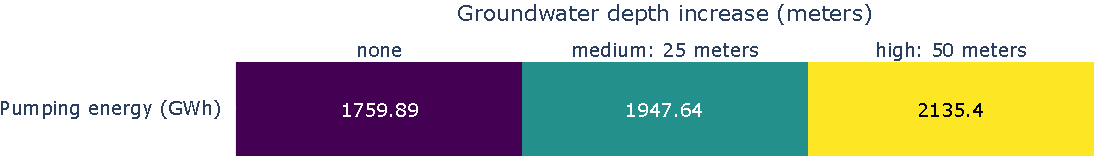
\includegraphics[width=\textwidth]{GWDSensitivityAll}
	\caption{Energy requirements for pumping change due to groundwater depth increase. This was calculated for Scenario 1 and all pumping requirements throughout the basin were aggregated}
	\label{fig:gwdsensall}
\end{figure} 
\newpage

\begin{figure}[!h]
	\centering
	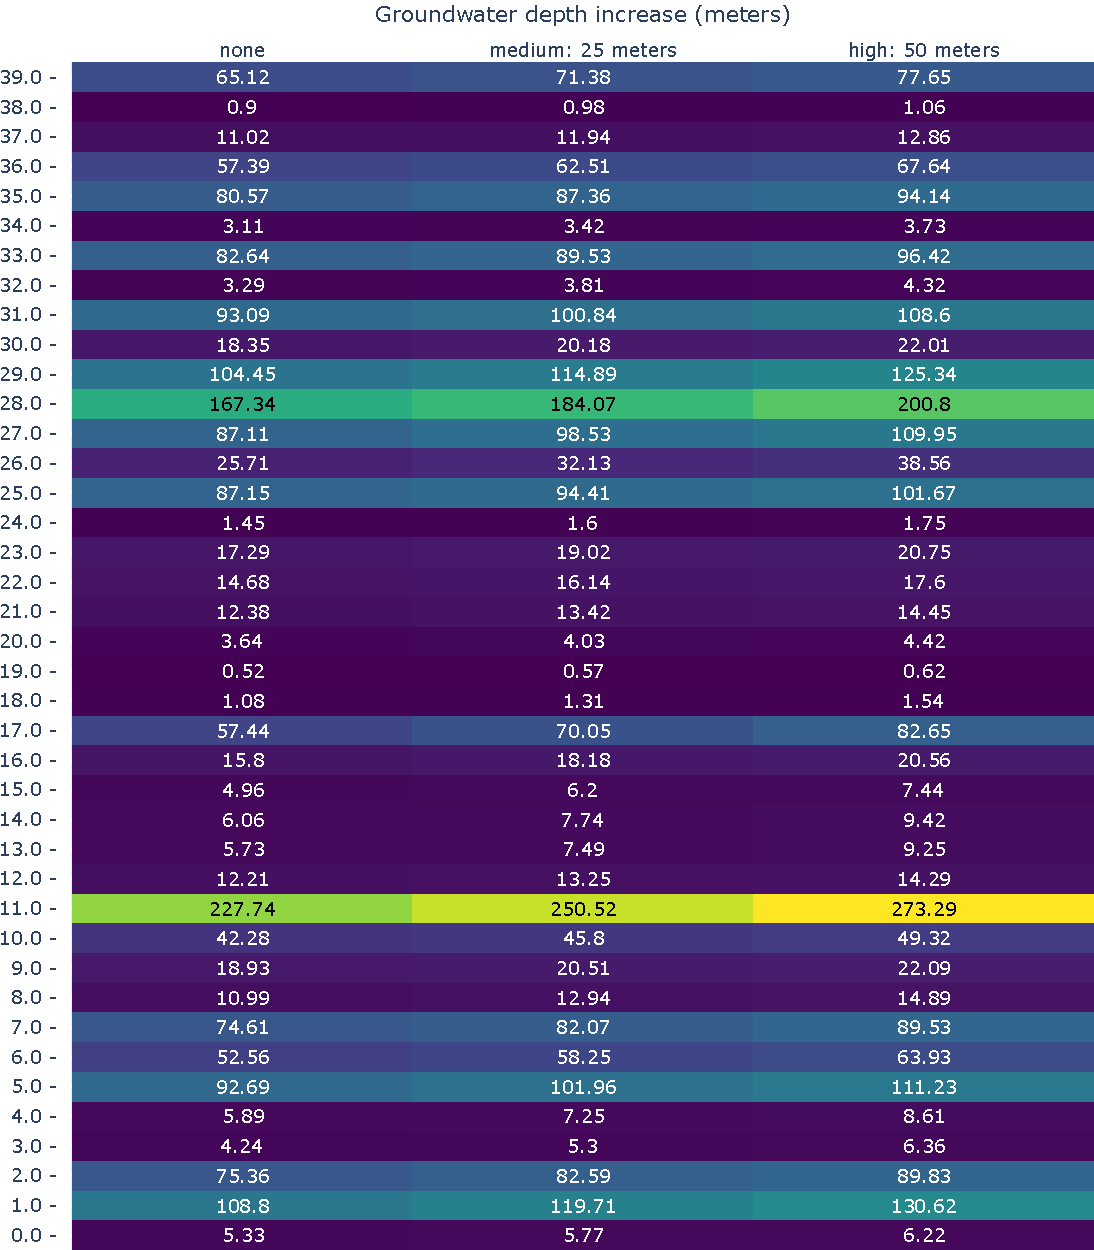
\includegraphics[width=\textwidth]{GWDSensitivityClusters}
	\caption{Energy requirements for pumping change due to groundwater depth increase. This was calculated for Scenario 1 for each cluster.}
	\label{fig:gwdsensclusters}
\end{figure} 
\newpage

\subsection{TDS content}
The effect that TDS content of groundwater has on desalination energy requirements, was evaluated through 2 different ways: 1) three levels of low, medium and high TDS concentration, varying the concentration levels by -50\%, 0\% and +50\% from current levels; and 2) by changing the TDS content threshold required to desalinate brackish water. The later values, were picked based on FAO recommendations for water quality for irrigation \cite{fao1985water}, where concentration below 450 mg/l have low or nonexistent impact, and concentrations from 450 to 2000 have slight to moderate impact. The outcomes of this analysis can be seen in figure 24 to 26. In general, the total content of TDS seems to have a higher effect on desalination energy demand.

\begin{figure}[!h]
	\centering
	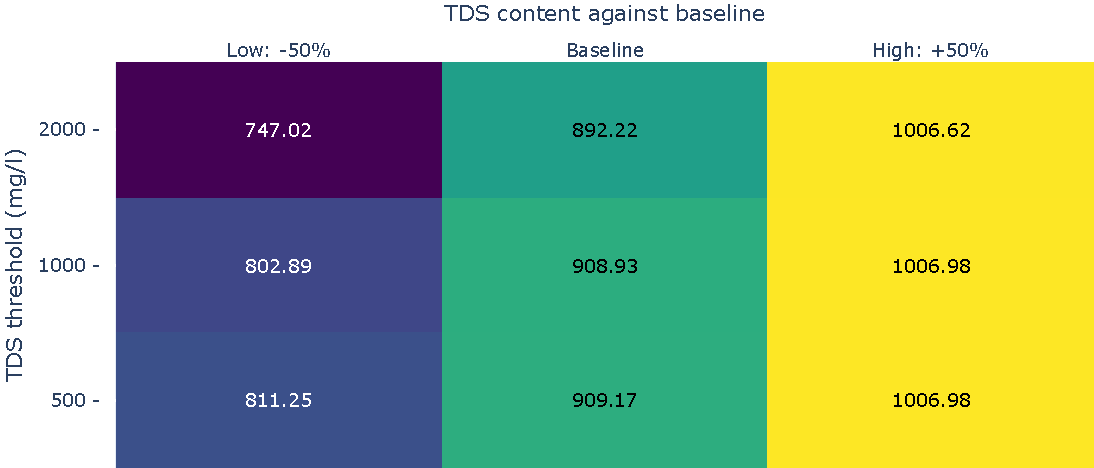
\includegraphics[width=\textwidth]{TDSSensitivityAll}
	\caption{Energy requirements for desalination (GWh/yr) due to TDS content change in groundwater. This was calculated for Scenario 1 and all desalination energy requirements throughout the basin were aggregated}
	\label{fig:tdssensall}
\end{figure} 
\newpage

\begin{figure}[!h]
	\centering
	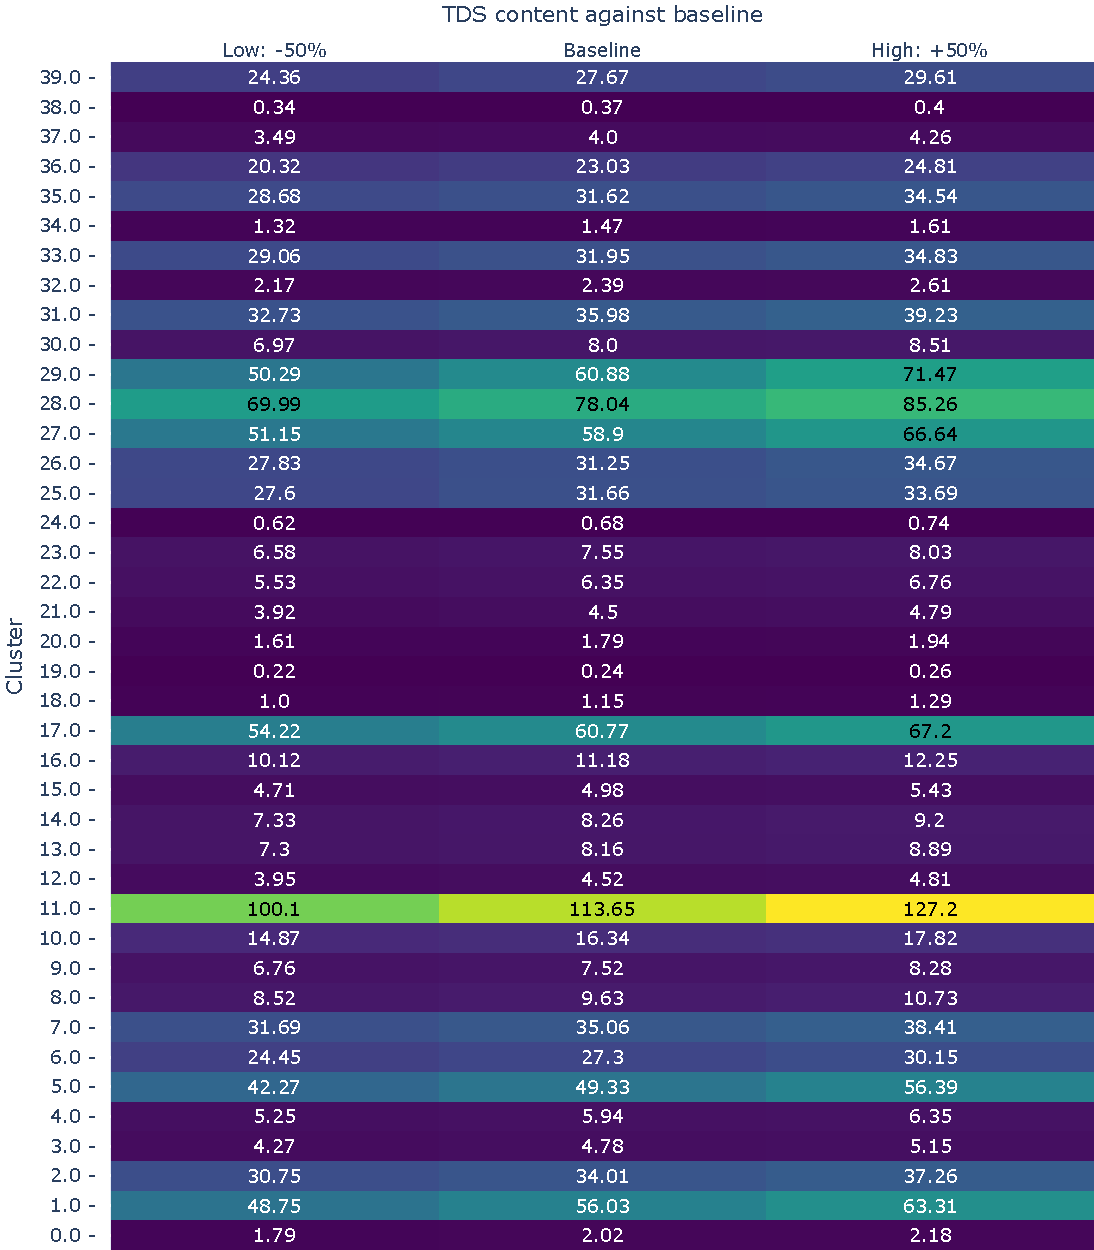
\includegraphics[width=\textwidth]{TDSSensitivityContentCluster}
	\caption{Energy requirements for desalination (GWh/yr) due to TDS content change in groundwater. This was calculated for Scenario 1 for each cluster}
	\label{fig:tdssenscluster}
\end{figure} 
\newpage

\begin{figure}[!h]
	\centering
	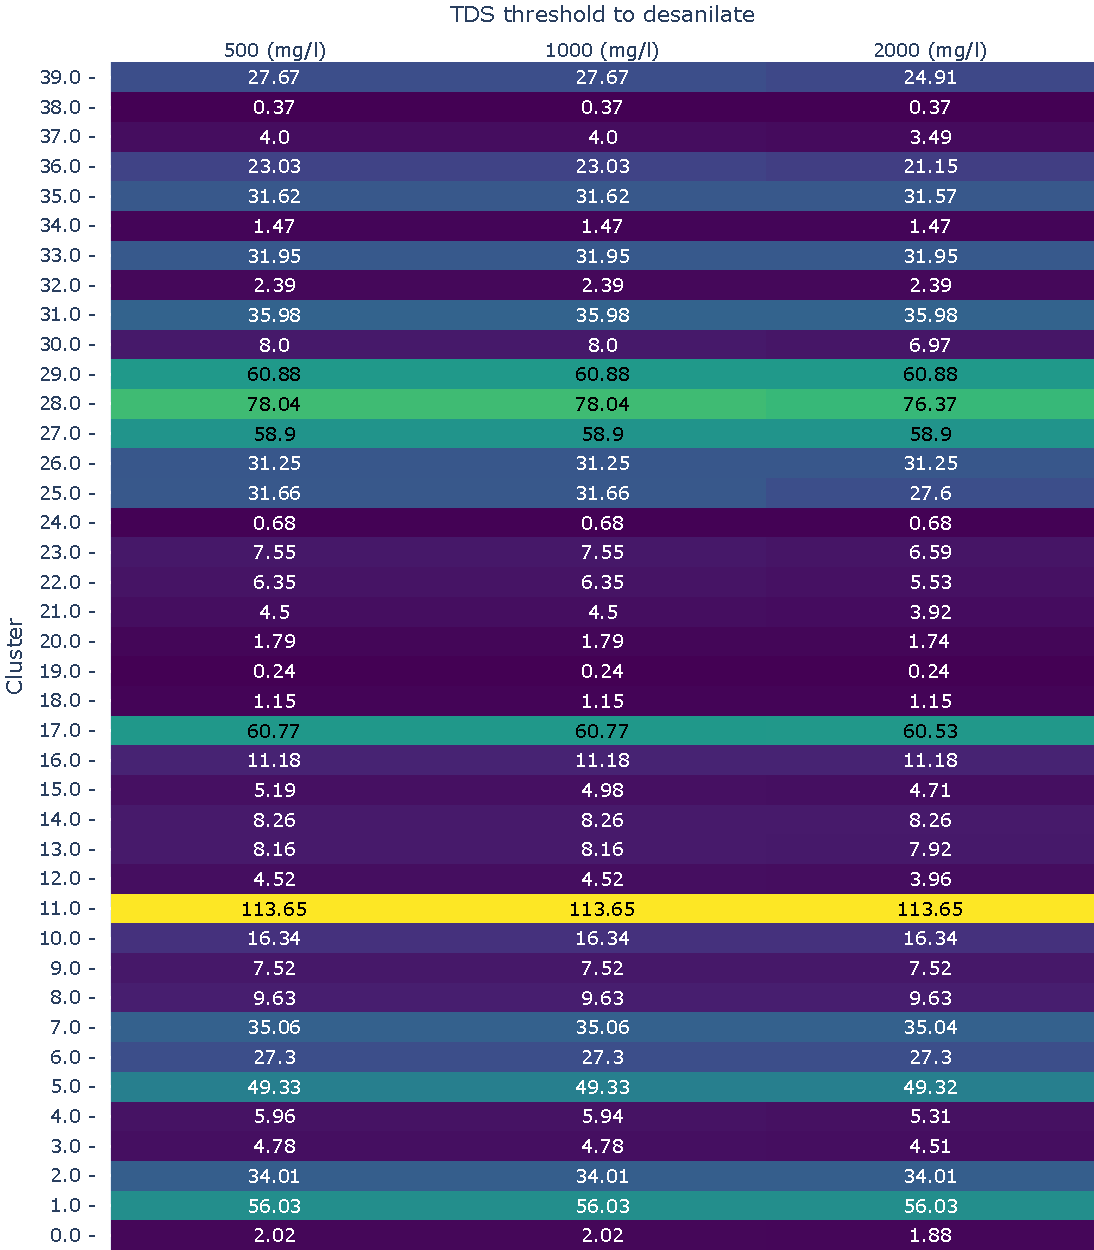
\includegraphics[width=\textwidth]{TDSSensitivityThresholdCluster}
	\caption{Energy requirements for desalination (GWh/yr) due to TDS threshold change to desalinate. This was calculated for Scenario 1 for each cluster}
	\label{fig:tdssensclusterthreshold}
\end{figure} 
\newpage

\subsection{Irrigated area growth}
For the sensitivity of irrigated area growth, three levels of growth in irrigated area were evaluated: low at 10\%, medium at 20\% and high at 40\%. These values were chosen taking as basis the intensification rates presented in \tref{tbl:provincialdata}, as if all in all region the intensification rate reaches 100\%, the overall change in irrigated area would be circa 20\%. Results are provided only for the overall aquifer. This is due to the fact that as the irrigated area was expanded, thus now the clustering algorithm may create different clusters. This makes some clusters to differ slightly between different growth scenarios. In general, irrigated area growth has important effects on total water withdrawals, total energy demand and total GWS, with increments of 25\%, 23\% and 23\% receptively in the worst case (figures 27 to 29). It is important to mention, that this values are substantially improved by the reuse of treated wastewater/tailwater in irrigation.

\begin{figure}[!h]
	\centering
	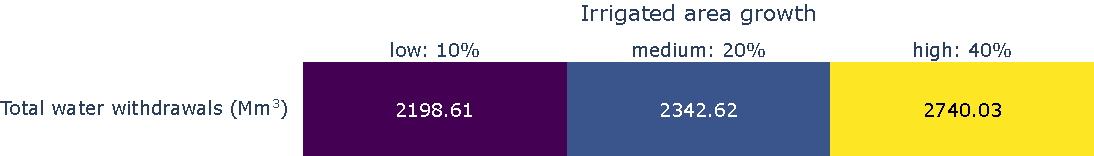
\includegraphics[width=\textwidth]{AreaSensitivityWaterAll}
	\caption{Total water withdrawals (Mm\textsuperscript{3}/yr). This was calculated for Scenario 1 and all values were aggregated throughout the basin.}
	\label{fig:areasenswaterall}
\end{figure} 

\begin{figure}[!h]
	\centering
	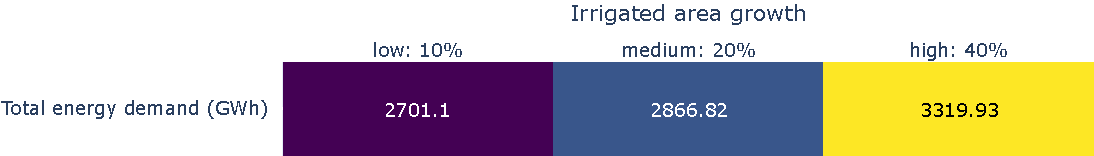
\includegraphics[width=\textwidth]{AreaSensitivityEnergyAll}
	\caption{Total energy demand (GWh/yr). This was calculated for Scenario 1 and all values were aggregated throughout the basin.}
	\label{fig:areasensenergyall}
\end{figure}

\begin{figure}[!h]
	\centering
	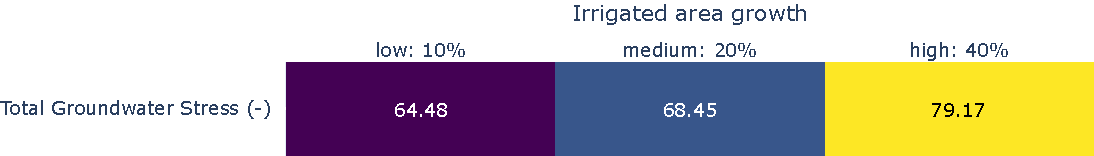
\includegraphics[width=\textwidth]{AreaSensitivityGWSAll}
	\caption{Total Groundwater Stress Indicator. This was calculated for Scenario 1 and all values were aggregated throughout the basin.}
	\label{fig:areasensgwsall}
\end{figure}

\newpage
\subsection{Population growth and domestic water use}
The sensitivity of population growth and domestic water use per capita change, were evaluated by two levels of growth: low: 2\% in Algeria and Libya and 1\% in Tunisia \cite{uneceReconcilingResourceUses2020}, and medium: 3\% in all countries. Moreover, three levels of domestic water use were accounted for based on ranges recommended by the World Health Organization to prevent health risks \cite{Householdwaterconsumption2014}. Outcomes show how domestic water use habits, seem to be more sensitive to the total water withdrawals and the associated energy requirements (figures 30-31 and 33-34). Moreover, it can be seen in \fref{fig:popasensleastcost} how the as domestic water demand increases due to population growth and water use per capita, treatment systems fitted for larger treatment capacity as extended aeration are chosen.

\begin{figure}[!h]
	\centering
	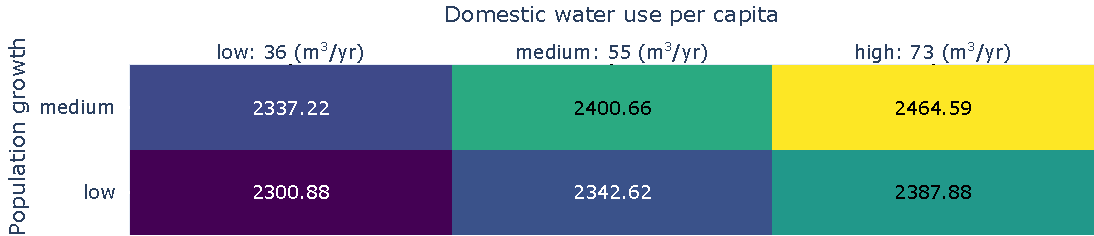
\includegraphics[width=\textwidth]{PopSensitivityWaterAll}
	\caption{Total water withdrawals (Mm\textsuperscript{3}/yr) change due to population growth and domestic water usage. This was calculated for Scenario 1 and all values were aggregated throughout the basin.}
	\label{fig:popasenswaterall}
\end{figure}

\begin{figure}[!h]
	\centering
	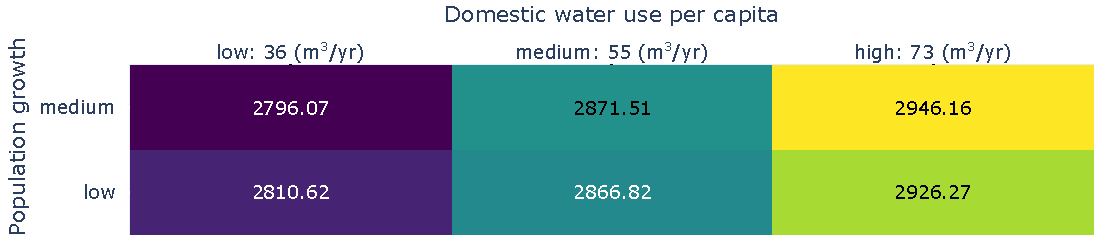
\includegraphics[width=\textwidth]{PopSensitivityEnergyAll}
	\caption{Total energy demand (GWh/yr)  due to population growth and domestic water usage. This was calculated for Scenario 1 and all values were aggregated throughout the basin.}
	\label{fig:popasensenergyall}
\end{figure}

\begin{figure}[!h]
	\centering
	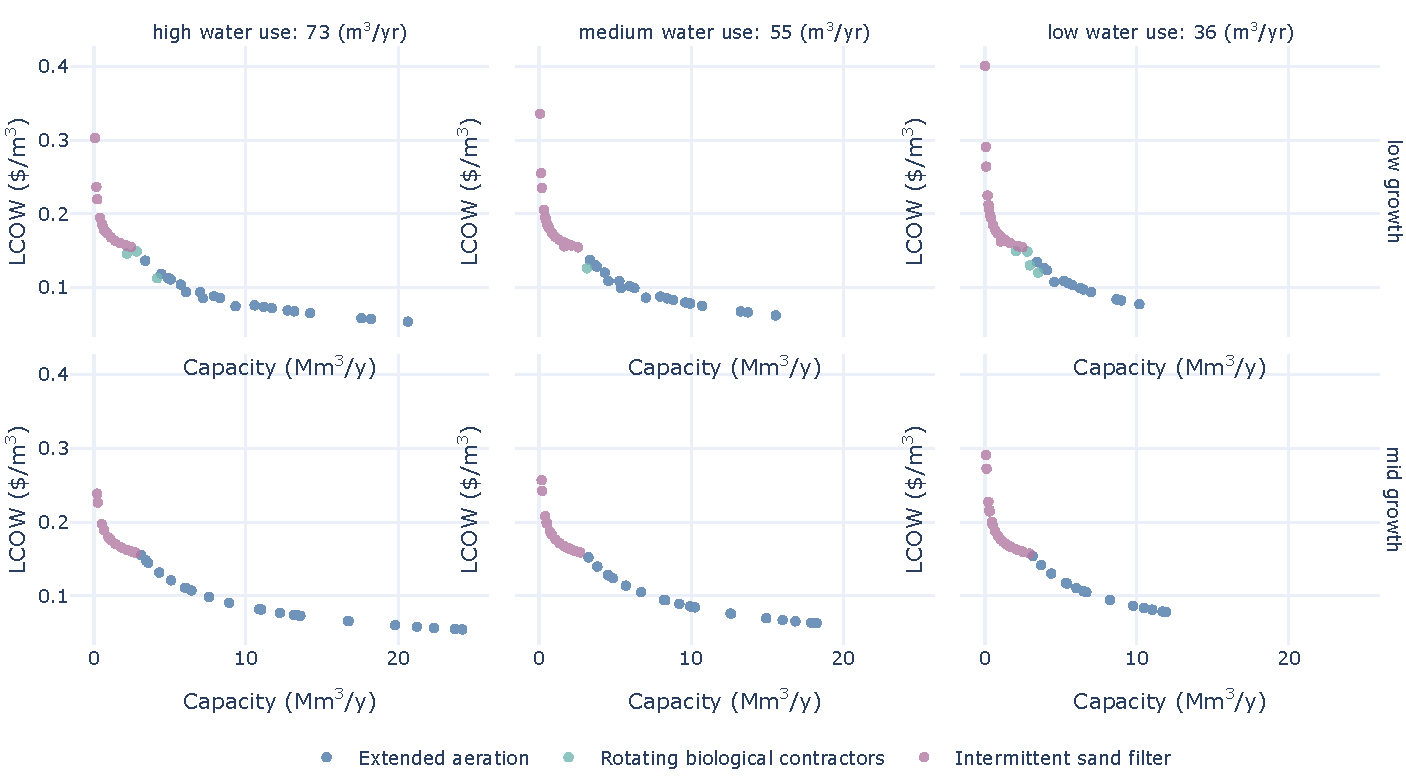
\includegraphics[width=\textwidth]{PopSensitivityLeastCost}
	\caption{Sensitivity of Lest-cost domestic wastewater treatment technologies chosen to changes in population growth and water use per capita.}
	\label{fig:popasensleastcost}
\end{figure}

\newpage
\begin{figure}[!h]
	\centering
	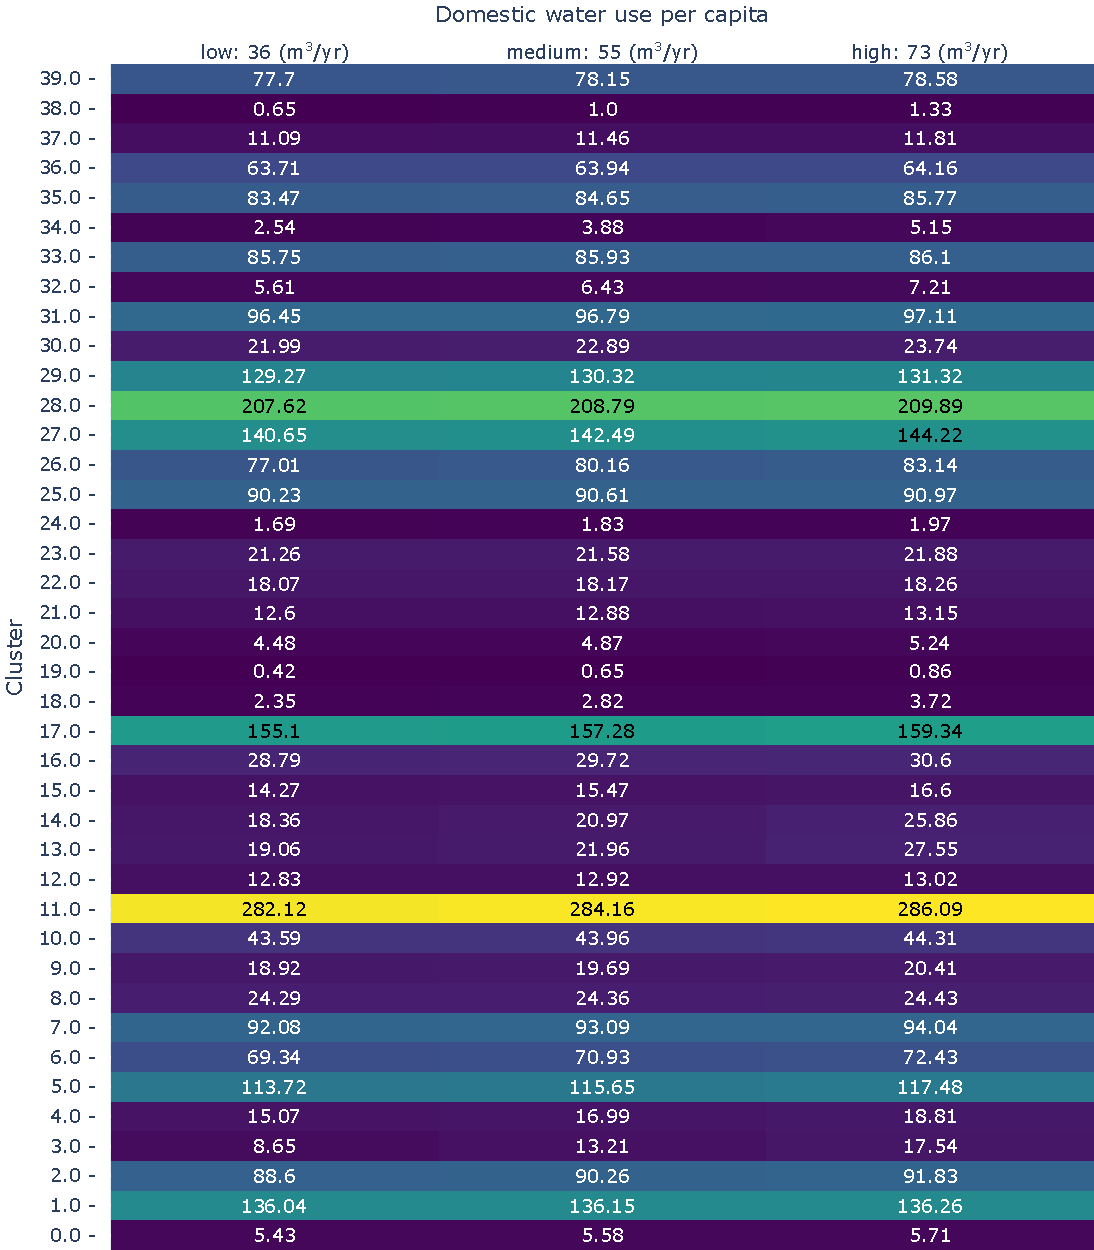
\includegraphics[width=\textwidth]{PopSensitivityWaterCluster}
	\caption{Total water withdrawals (Mm\textsuperscript{3}/yr) change per cluster due to population growth and domestic water usage.}
	\label{fig:popasenswatercluster}
\end{figure}

\newpage
\begin{figure}[!h]
	\centering
	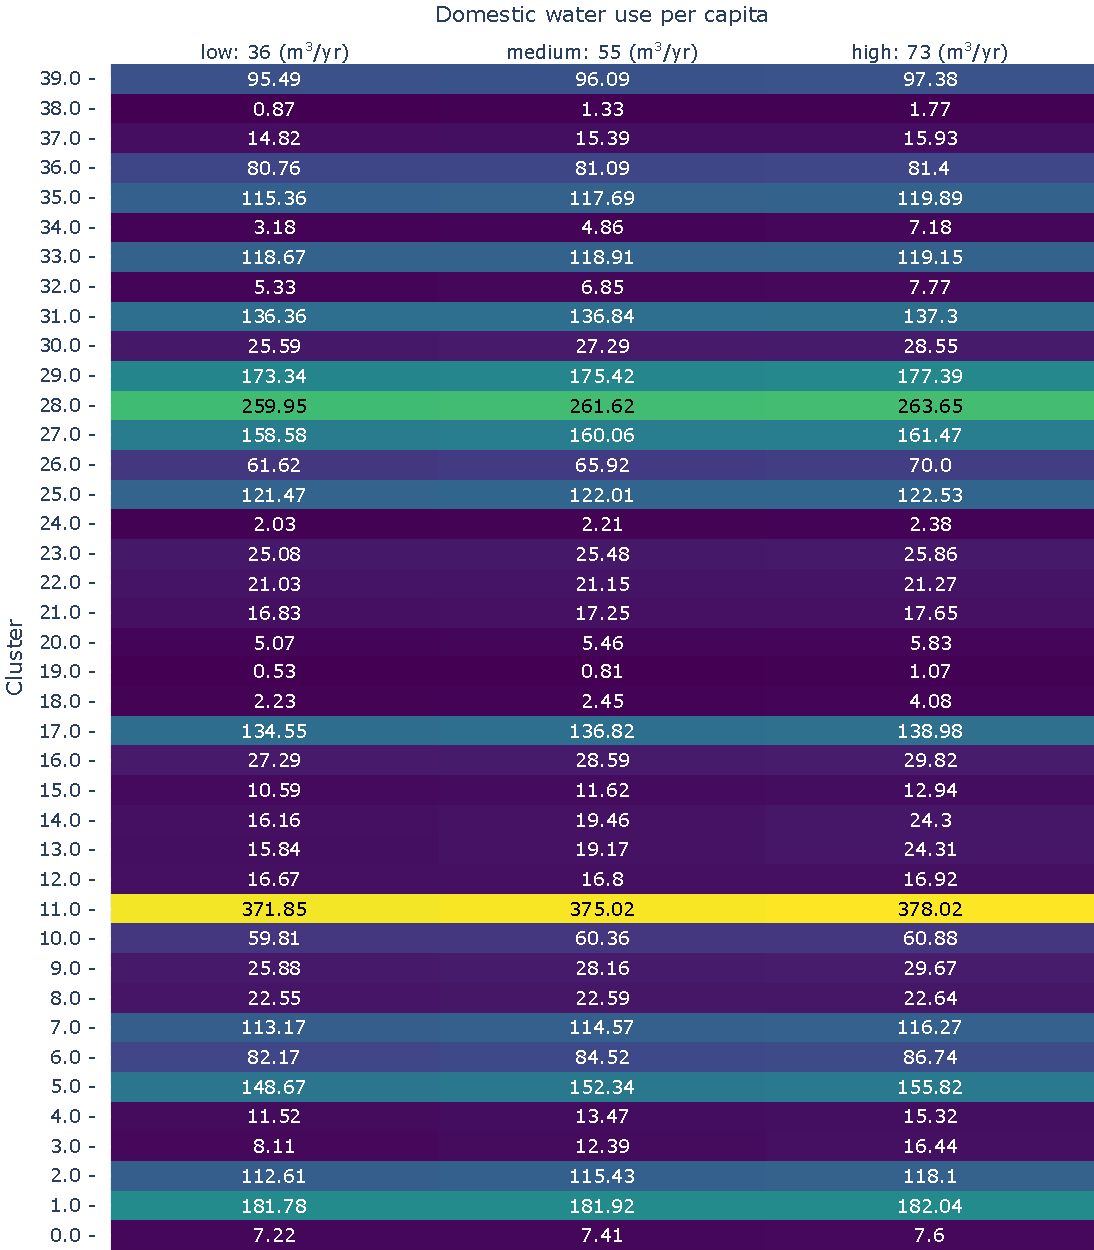
\includegraphics[width=\textwidth]{PopSensitivityEnergyCluster}
	\caption{Total energy demand (GWh/yr) per cluster due to population growth and domestic water usage}
	\label{fig:popasensenergycluster}
\end{figure}
\newpage

\begin{figure}[!h]
	\centering
	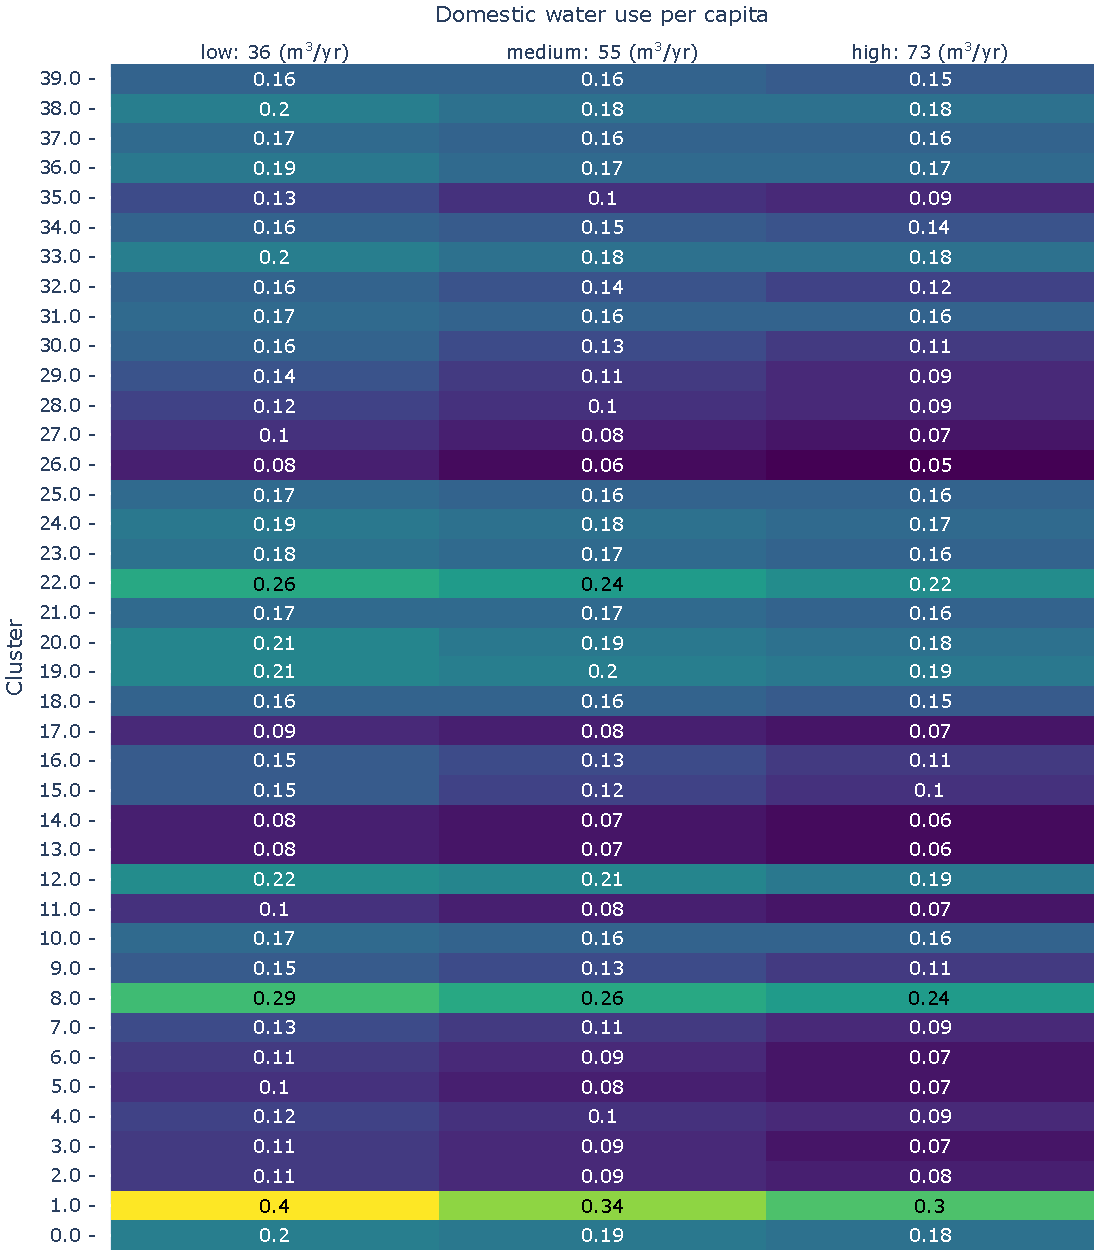
\includegraphics[width=\textwidth]{PopSensitivityLCOWCluster}
	\caption{Sensitivity of LCOW (\$/m\textsuperscript{3}) value of domestic wastewater treatment technologies chosen, to changes in population growth and water use per capita.}
	\label{fig:popasenslcowcluster}
\end{figure}

\clearpage
\subsection{Discount rate}
Finally, the sensitivity of the scenario analysis results to the discount rate was calculated. The paper uses a discount rate of 5\%, which is higher than a ‘social discount rate’\footnote{A Social Discount Rate is seen as a measure of a country’s value of future costs and benefits, and is related to the notion of promoted sustainability.} of 3\% but lower than a typical business discount rate of 8\%. As visible in \fref{fig:drsensall} and \fref{fig:drsenscluster} a different discount rate influence the levelized LCOW, however it does not change significantly the dynamics of the results (technologies chosen).

\begin{figure}[!h]
	\centering
	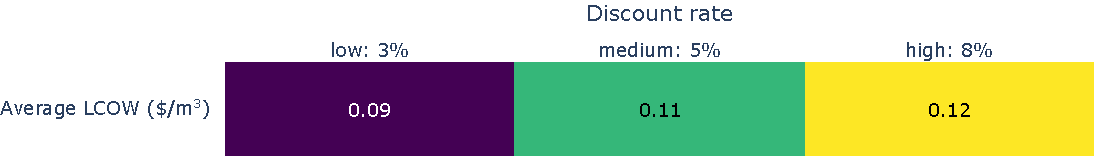
\includegraphics[width=\textwidth]{DRSensitivityAll}
	\caption{Average Levelized Cost of Water (LCOW) (\$/m\textsuperscript{3}) calculated for for different discount rates. The values average is reported for the NWSAS.}
	\label{fig:drsensall}
\end{figure}

\begin{figure}[!h]
	\centering
	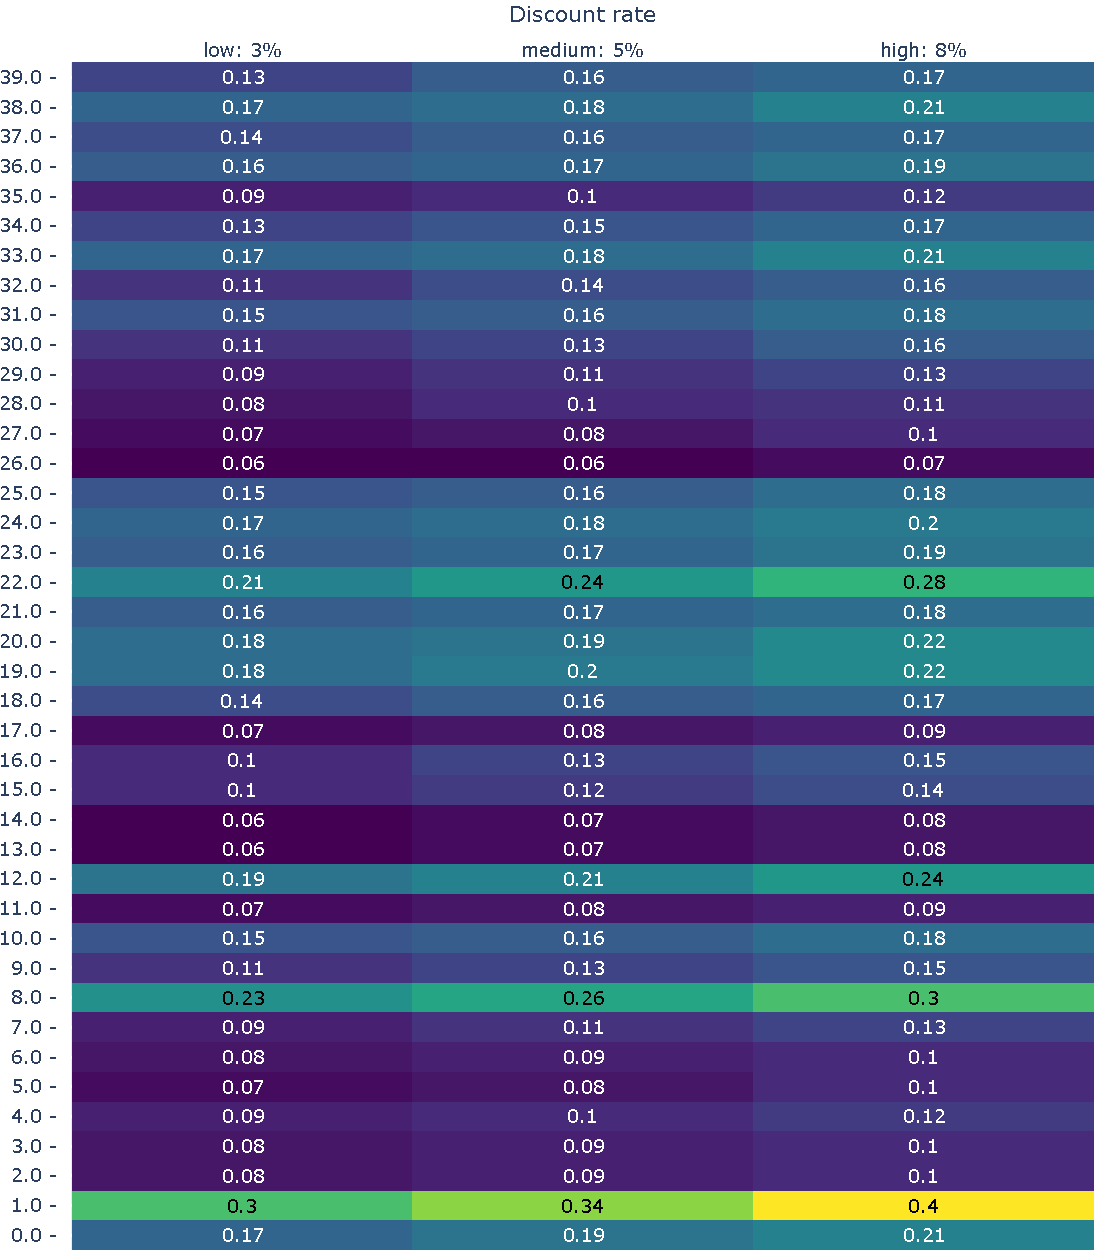
\includegraphics[width=\textwidth]{DRSensitivityCluster}
	\caption{Levelized Cost of Water (LCOW) (\$/m\textsuperscript{3}) calculated for for different discount rates. The values are reported for each cluster.}
	\label{fig:drsenscluster}
\end{figure}
\newpage


\newcommand{\newblock}{}
\bibliography{References}
\bibliographystyle{unsrtnat}

\end{document}